\documentclass[,man,floatsintext]{apa6}
\usepackage{lmodern}
\usepackage{amssymb,amsmath}
\usepackage{ifxetex,ifluatex}
\usepackage{fixltx2e} % provides \textsubscript
\ifnum 0\ifxetex 1\fi\ifluatex 1\fi=0 % if pdftex
  \usepackage[T1]{fontenc}
  \usepackage[utf8]{inputenc}
\else % if luatex or xelatex
  \ifxetex
    \usepackage{mathspec}
  \else
    \usepackage{fontspec}
  \fi
  \defaultfontfeatures{Ligatures=TeX,Scale=MatchLowercase}
\fi
% use upquote if available, for straight quotes in verbatim environments
\IfFileExists{upquote.sty}{\usepackage{upquote}}{}
% use microtype if available
\IfFileExists{microtype.sty}{%
\usepackage{microtype}
\UseMicrotypeSet[protrusion]{basicmath} % disable protrusion for tt fonts
}{}
\usepackage{hyperref}
\hypersetup{unicode=true,
            pdftitle={Learning to Interpret a Disjunction},
            pdfauthor={Masoud Jasbi, Akshay Jaggi, \& Michael C. Frank},
            pdfkeywords={keywords},
            pdfborder={0 0 0},
            breaklinks=true}
\urlstyle{same}  % don't use monospace font for urls
\usepackage{longtable,booktabs}
\usepackage{graphicx,grffile}
\makeatletter
\def\maxwidth{\ifdim\Gin@nat@width>\linewidth\linewidth\else\Gin@nat@width\fi}
\def\maxheight{\ifdim\Gin@nat@height>\textheight\textheight\else\Gin@nat@height\fi}
\makeatother
% Scale images if necessary, so that they will not overflow the page
% margins by default, and it is still possible to overwrite the defaults
% using explicit options in \includegraphics[width, height, ...]{}
\setkeys{Gin}{width=\maxwidth,height=\maxheight,keepaspectratio}
\IfFileExists{parskip.sty}{%
\usepackage{parskip}
}{% else
\setlength{\parindent}{0pt}
\setlength{\parskip}{6pt plus 2pt minus 1pt}
}
\setlength{\emergencystretch}{3em}  % prevent overfull lines
\providecommand{\tightlist}{%
  \setlength{\itemsep}{0pt}\setlength{\parskip}{0pt}}
\setcounter{secnumdepth}{0}
% Redefines (sub)paragraphs to behave more like sections
\ifx\paragraph\undefined\else
\let\oldparagraph\paragraph
\renewcommand{\paragraph}[1]{\oldparagraph{#1}\mbox{}}
\fi
\ifx\subparagraph\undefined\else
\let\oldsubparagraph\subparagraph
\renewcommand{\subparagraph}[1]{\oldsubparagraph{#1}\mbox{}}
\fi

%%% Use protect on footnotes to avoid problems with footnotes in titles
\let\rmarkdownfootnote\footnote%
\def\footnote{\protect\rmarkdownfootnote}


  \title{Learning to Interpret a Disjunction}
    \author{Masoud Jasbi\textsuperscript{1}, Akshay Jaggi\textsuperscript{2}, \& Michael C. Frank\textsuperscript{2}}
    \date{}
  
\shorttitle{Learning Disjunction}
\affiliation{
\vspace{0.5cm}
\textsuperscript{1} Harvard University\\\textsuperscript{2} Stanford University}
\keywords{keywords\newline\indent Word count: X}
\usepackage{csquotes}
\usepackage{upgreek}
\captionsetup{font=singlespacing,justification=justified}

\usepackage{longtable}
\usepackage{lscape}
\usepackage{multirow}
\usepackage{tabularx}
\usepackage[flushleft]{threeparttable}
\usepackage{threeparttablex}

\newenvironment{lltable}{\begin{landscape}\begin{center}\begin{ThreePartTable}}{\end{ThreePartTable}\end{center}\end{landscape}}

\makeatletter
\newcommand\LastLTentrywidth{1em}
\newlength\longtablewidth
\setlength{\longtablewidth}{1in}
\newcommand{\getlongtablewidth}{\begingroup \ifcsname LT@\roman{LT@tables}\endcsname \global\longtablewidth=0pt \renewcommand{\LT@entry}[2]{\global\advance\longtablewidth by ##2\relax\gdef\LastLTentrywidth{##2}}\@nameuse{LT@\roman{LT@tables}} \fi \endgroup}


\usepackage{lineno}

\linenumbers

\authornote{Add complete departmental affiliations for each author here. Each new line herein must be indented, like this line.

Enter author note here.

Correspondence concerning this article should be addressed to Masoud Jasbi, Postal address. E-mail: \href{mailto:masoud_jasbi@fas.harvard.edu}{\nolinkurl{masoud\_jasbi@fas.harvard.edu}}}

\abstract{
At first glance, children's word learning appears to be mostly a problem of learning words like \emph{dog} and \emph{run}. However, it is small words like \emph{and} and \emph{or} that enable the construction of complex combinatorial language. How do children learn the meaning of these function words? Using transcripts of parent-child interactions, we investigate the cues in child-directed speech that can inform the interpretation and acquisition of the connective \emph{or} which has a particularly challenging semantics. Study 1 finds that, despite its low overall frequency, children can use \emph{or} close to parents' rate by age 4, in some speech acts. Study 2 uses annotations of a subset of parent-child interactions to show that disjunctions in child-directed speech are accompanied by reliable cues to the correct interpretation (exclusive vs.~inclusive). We present a decision-tree model that learns from a handful of annotated examples to correctly predict the interpretation of a disjunction. These studies suggest that conceptual and prosodic cues in child-directed speech can provide information for the acquisition of functional categories like disjunction.


}

\begin{document}
\maketitle

\hypertarget{introduction}{%
\section{Introduction}\label{introduction}}

Word learning is commonly construed as the process of isolating a word form, selecting a meaning from a set of potential meanings, and mapping the word to the selected meaning ({\textbf{???}}). For example, a father holding a baby may point to a squirrel and say \enquote{look at the squirrel!} The baby -- already familiar with the phrase \enquote{look at the} -- should recognize the novel word \emph{squirrel}, consider some potential referents (e.g tree, squirrel, chair, etc.) and select the right referent using the available cues, in this case the father's pointing. While there has been a lot of research on cues and mechanisms that help children's acquisition of content words such as \emph{squirrel}, \emph{red}, and \emph{run}, we know little about cues and mechanisms that can assist children in learning the meaning of function words such as \emph{and}, \emph{the}, \emph{of}, and \emph{or}. In this study, we focus on the disjunction word \emph{or} and provide a novel learning account that uses salient cues to learn the interpretations of disjunction in English.

We argue that the case of \emph{or}, shows the \ldots{}

\hypertarget{previous-literature}{%
\subsection{Previous Literature}\label{previous-literature}}

To our knowledge, only one study has looked at parents' and children's spontaneous productions of logical connectives \emph{and} and \emph{or} before. Morris (2008) investigated the use of these connectives by parents and children between the ages of 2;0 and 5;0, using 240 transcriptions of audiotaped exchanges obtained in the CHILDES database. Each connective was analyzed with respect to its frequency, sentence type, and meaning (or use). The study found that overall, \emph{and} was approximately 12.8 times more likely to be produced than \emph{or}. The connective \emph{and} appeared predominantly in statements (more than 90\% of the time) while \emph{or} was most common in questions (more than 85\% of the time). Children started producing \emph{and} at 2 years and \emph{or} at 2.5 years of age.

Regarding the meaning of the connectives, Morris (2008) adopted a usage-based (item-based) approach (Levy \& Nelson, 1994; Tomasello, 2003) and predicted that children start producing connectives with a single \enquote{core meaning} (also referred to as \enquote{use} or \enquote{communicative function}). He also predicted that the core meanings mirror the most frequent usage/meaning of the connectives in child-directed speech, and that children acquire more meanings of the connectives as they grow older. He found that children started producing \emph{and} as conjunction at 2, and \emph{or} as exclusive disjunction at 2.5 years of age. In line with the predictions of the usage-based account, he found that these two meanings are the most frequent meanings in parents' speech. For disjunction, 75-80\% of the \emph{or}-examples children heard recevied an exclusive interpretation. Finally, as children grew older, they started using connectives to convey additional meanings such as inclusive disjunction for \emph{or} and temporal conjunction for \emph{and}. However, the inclusive use of \emph{or} was extremely rare in adults, and children barely produced it even at age 5. Morris (2008) argued that the development of connectives conforms to the predictions of a usage-based account and that in the first five years of children's development, the (core) meaning of disjunction is exclusive.

However, a series of experimental studies have found that children between the ages of 3 and 5 interpret \emph{or} as inclusive disjunction in a variety of linguistic contexts including negative sentences (Crain, Gualmini, \& Meroni, 2000), conditional sentences (Gualmini et al., 2000a), restriction and nuclear scope of the universal quantifier \emph{every} (Chierchia, Crain, Guasti, Gualmini, \& Meroni, 2001; Chierchia et al., 2004), nuclear scope of the negative quantifier \emph{none} (Gualmini \& Crain, 2002), restriction and nuclear scope of \emph{not every} (Notley et al., 2012a), and prepositional phrases headed by \emph{before} (Notley et al., 2012b). These studies almost unanimously claim that at least in declarative sentences, the inclusive interpretation of \emph{or} emerges earlier than the exclusive interpretation.

\begin{longtable}[]{@{}ccc@{}}
\caption{\label{tab:providence}}\tabularnewline
\toprule
\begin{minipage}[b]{0.25\columnwidth}\centering
Premise\strut
\end{minipage} & \begin{minipage}[b]{0.25\columnwidth}\centering
Age Range\strut
\end{minipage} & \begin{minipage}[b]{0.42\columnwidth}\centering
Studies\strut
\end{minipage}\tabularnewline
\midrule
\endfirsthead
\toprule
\begin{minipage}[b]{0.25\columnwidth}\centering
Premise\strut
\end{minipage} & \begin{minipage}[b]{0.25\columnwidth}\centering
Age Range\strut
\end{minipage} & \begin{minipage}[b]{0.42\columnwidth}\centering
Studies\strut
\end{minipage}\tabularnewline
\midrule
\endhead
\begin{minipage}[t]{0.25\columnwidth}\centering
Premise 1\strut
\end{minipage} & \begin{minipage}[t]{0.25\columnwidth}\centering
Most examples of disjunction children hear are exclusive (XOR)\strut
\end{minipage} & \begin{minipage}[t]{0.42\columnwidth}\centering
Morris (2008)\strut
\end{minipage}\tabularnewline
\begin{minipage}[t]{0.25\columnwidth}\centering
Premise 2\strut
\end{minipage} & \begin{minipage}[t]{0.25\columnwidth}\centering
In truth value judgment tasks with declarative sentences, preschool children interpret a disjunction as inclusive\strut
\end{minipage} & \begin{minipage}[t]{0.42\columnwidth}\centering
Crain (2012)\strut
\end{minipage}\tabularnewline
\begin{minipage}[t]{0.25\columnwidth}\centering
Paradox\strut
\end{minipage} & \begin{minipage}[t]{0.25\columnwidth}\centering
How can children learn the inclusive interpretation of disjunction if they rarely hear it?\strut
\end{minipage} & \begin{minipage}[t]{0.42\columnwidth}\centering
Crain (2012)\strut
\end{minipage}\tabularnewline
\bottomrule
\end{longtable}

The findings of these studies as well as those of Morris (2008) give rise to what we call \enquote{the paradox of learning disjunction}: given Morris (2008)'s finding that the majority of \emph{or} examples children hear are exclusive, how can children learn to interpret \emph{or} as inclusive? To address this paradox, Crain (2012) put forth the logical nativist theory of connective acquisition. In logical nativism, the language faculty contains information regarding what connective meanings are allowed for connective words crosslinguistically. Crain (2012) considered it unlikely that children learn the meaning of \emph{or} from the examples they hear in adult usage. Instead, he argued that children rely on an innate knowledge that the meaning of disjunction words in natural languages must be inclusive. In other words, upon hearing a connective word, children consider inclusive disjunction as a viable candidate for its meaning but not exclusive disjunction. In this account, the exclusive interpretation emerges as part of children's pragmatic development, and after they have mastered the inclusive semantics of disjunction.

While logical nativism addresses the paradox of learning disjunction, it does not provide an explanation for cases where children interpret disjunction as exclusive. Morris (2008) reported that in his study, the vast majority of children's \emph{or} productions between the ages of 2 and 5 years received an exclusive interpretation. This is not expected if preschool children consider disjunction to be inclusive. Second, other experimental studies, especially those testing disjunction in commands, find that preschool children interpret it as exclusive (Braine \& Rumain, 1981; Johansson \& Sjolin, 1975). For example, in response to a command such as \enquote{give me the doll or the dog}, children as young as three- and four-years-old give one of the objects and not both. It is not clear how children derive exclusive interpretation within the nativist theory.

Figure \ref{fig:theories} summarizes the usage-based and nativist approaches to the acquisition of disjunction. The major difference between them is their assumptions on the learners' semantic hypothesis space for \emph{or}. The usage-based account considers a wide array of meanings to be available for mapping, including different flavors of conjunction such as \enquote{temporal conjunction} (e.g.~Bob pressed the key and (then) the door opened) and \enquote{explanatory conjunction}. The nativist account limits the hypothesis space to binary logical connectives, more specifically to those commonly used in standard propositional logic: inclusive disjunction, conjunction, and material implication. Both accounts agree that the input favors the exclusive interpretation of disjunction. The usage-based account concludes that children's early mappings mirror this input. The nativist account suggests that innate biases towards the inclusive meaning and against the exclusive interpretation result in an inclusive semantics for \emph{or} in children's early mappings.

\begin{figure}[tb]

{\centering 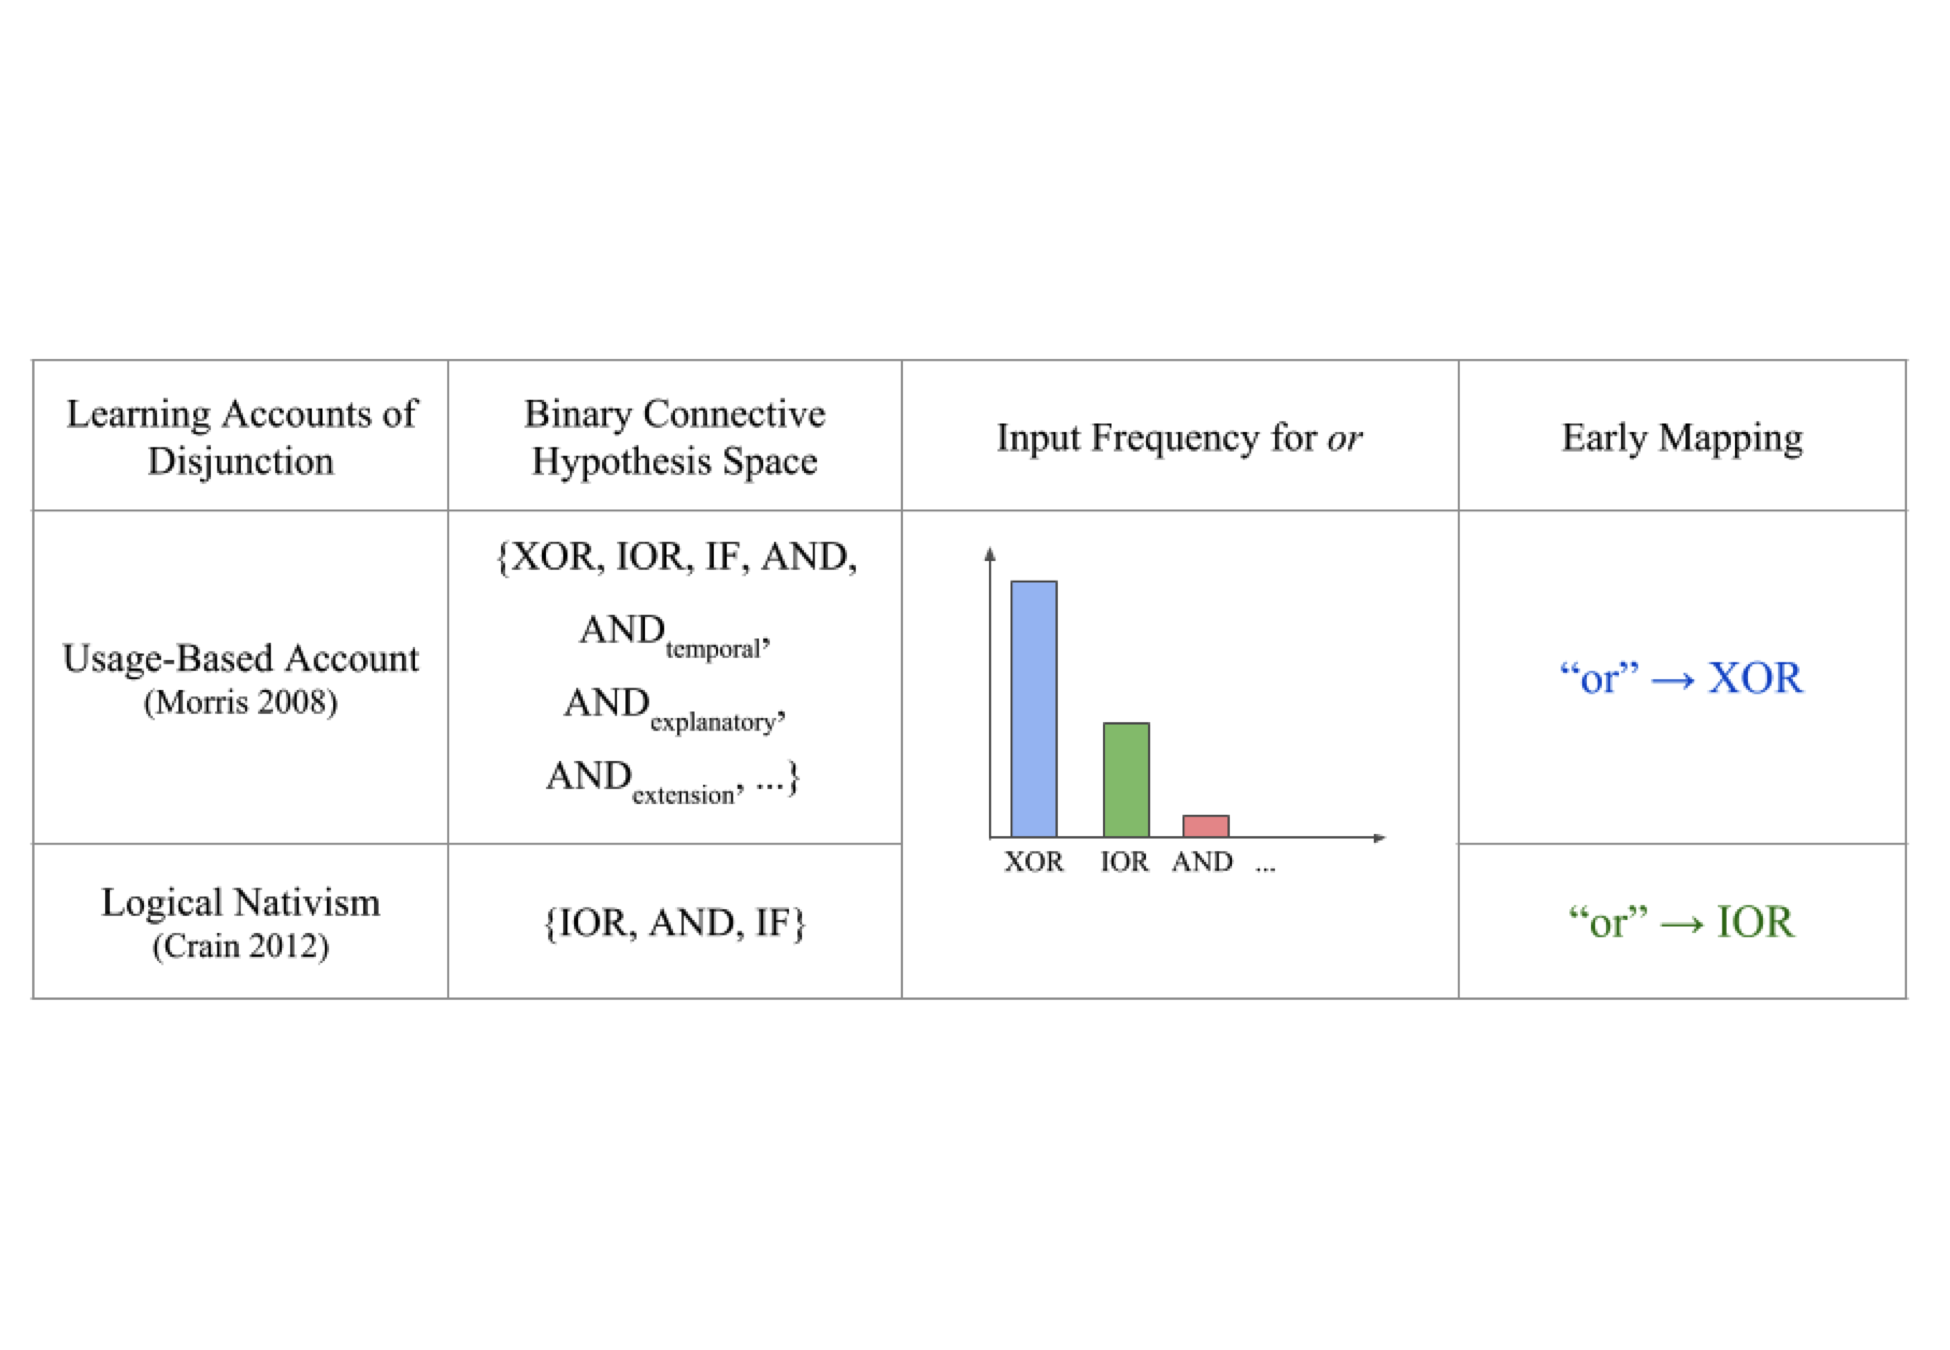
\includegraphics{figs/theories-1} 

}

\caption{Summary of the usage-based and nativist approaches to the acquisition of disjunction.}\label{fig:theories}
\end{figure}

\hypertarget{current-study}{%
\subsection{Current Study}\label{current-study}}

We propose a new account for children's acquisition of disjunction. Figure \ref{fig:cueBasedAccount} shows the summary of this account which we call cue-based context-dependent mapping. It is inspired by the usage-based and nativist accounts of disjunction and shares many of their insights. Similar to the nativist account, we assume that the semantic hypothesis space includes binary logical relations. However, we do not limit the hypothesis space further and do not bias the learning towards the inclusive meaning. We will show that the input will do this.

Similar to usage based proposals, our account maps more complex constructions to meanings rather than the word directly. Therefore, the mapping unites are similar to feature matrices. The learner can later extract commonalities across these mappings and extract a core meaning. However, the early mappings do not have any \enquote{core} meaning as opposed to what the usage-based account proposes.

The major point of departure from previous accounts is the mechanism of learning. While in pervious accounts the most frequent meaning in the input was mapped to the connective word, in our account the input is partitions or broken down by a set of salient cues that designate the context of use. Mapping is done based on the cues that accompany the connective word.

We show that this account resolves the paradox of learning disjunction explained earlier.

The purpose of this paper is to provide a novel resolution to the paradox of learning disjunction. The current consensus in the litereature - usage-based and nativist - is that learning from child-directed speech will result in an exclusive interpretation for disjunciton. We argue that this is true only under the vanilla model of form-meaning mapping.

We show that the frequency of \emph{or}'s We provide a model that learns to interpret a disjunciton as inclusive or exclusive depending on the cues available in the context.

Here we present 4 studies. The first study focuses on the frequency of disjunction in adult-adult interactions. The second study looks at the frequency of disjunction in parent-child interactions. The third study selects a sample of parent-child interactions and takes a closer look at the interpretations of disjunction in context. The fourth study uses the annotations developed in the third study to train a computational model that learns the interpretation of a disjunction based on the cues that accompany it. We show that a learner that pays attention to the interpretive cues accompanying disjunction can learn to interpret it successfully as inclusive or exclusive.

Readers who are mainly interested in our proposed account and computational modeling could skip to study 4.

\begin{figure}[tb]

{\centering 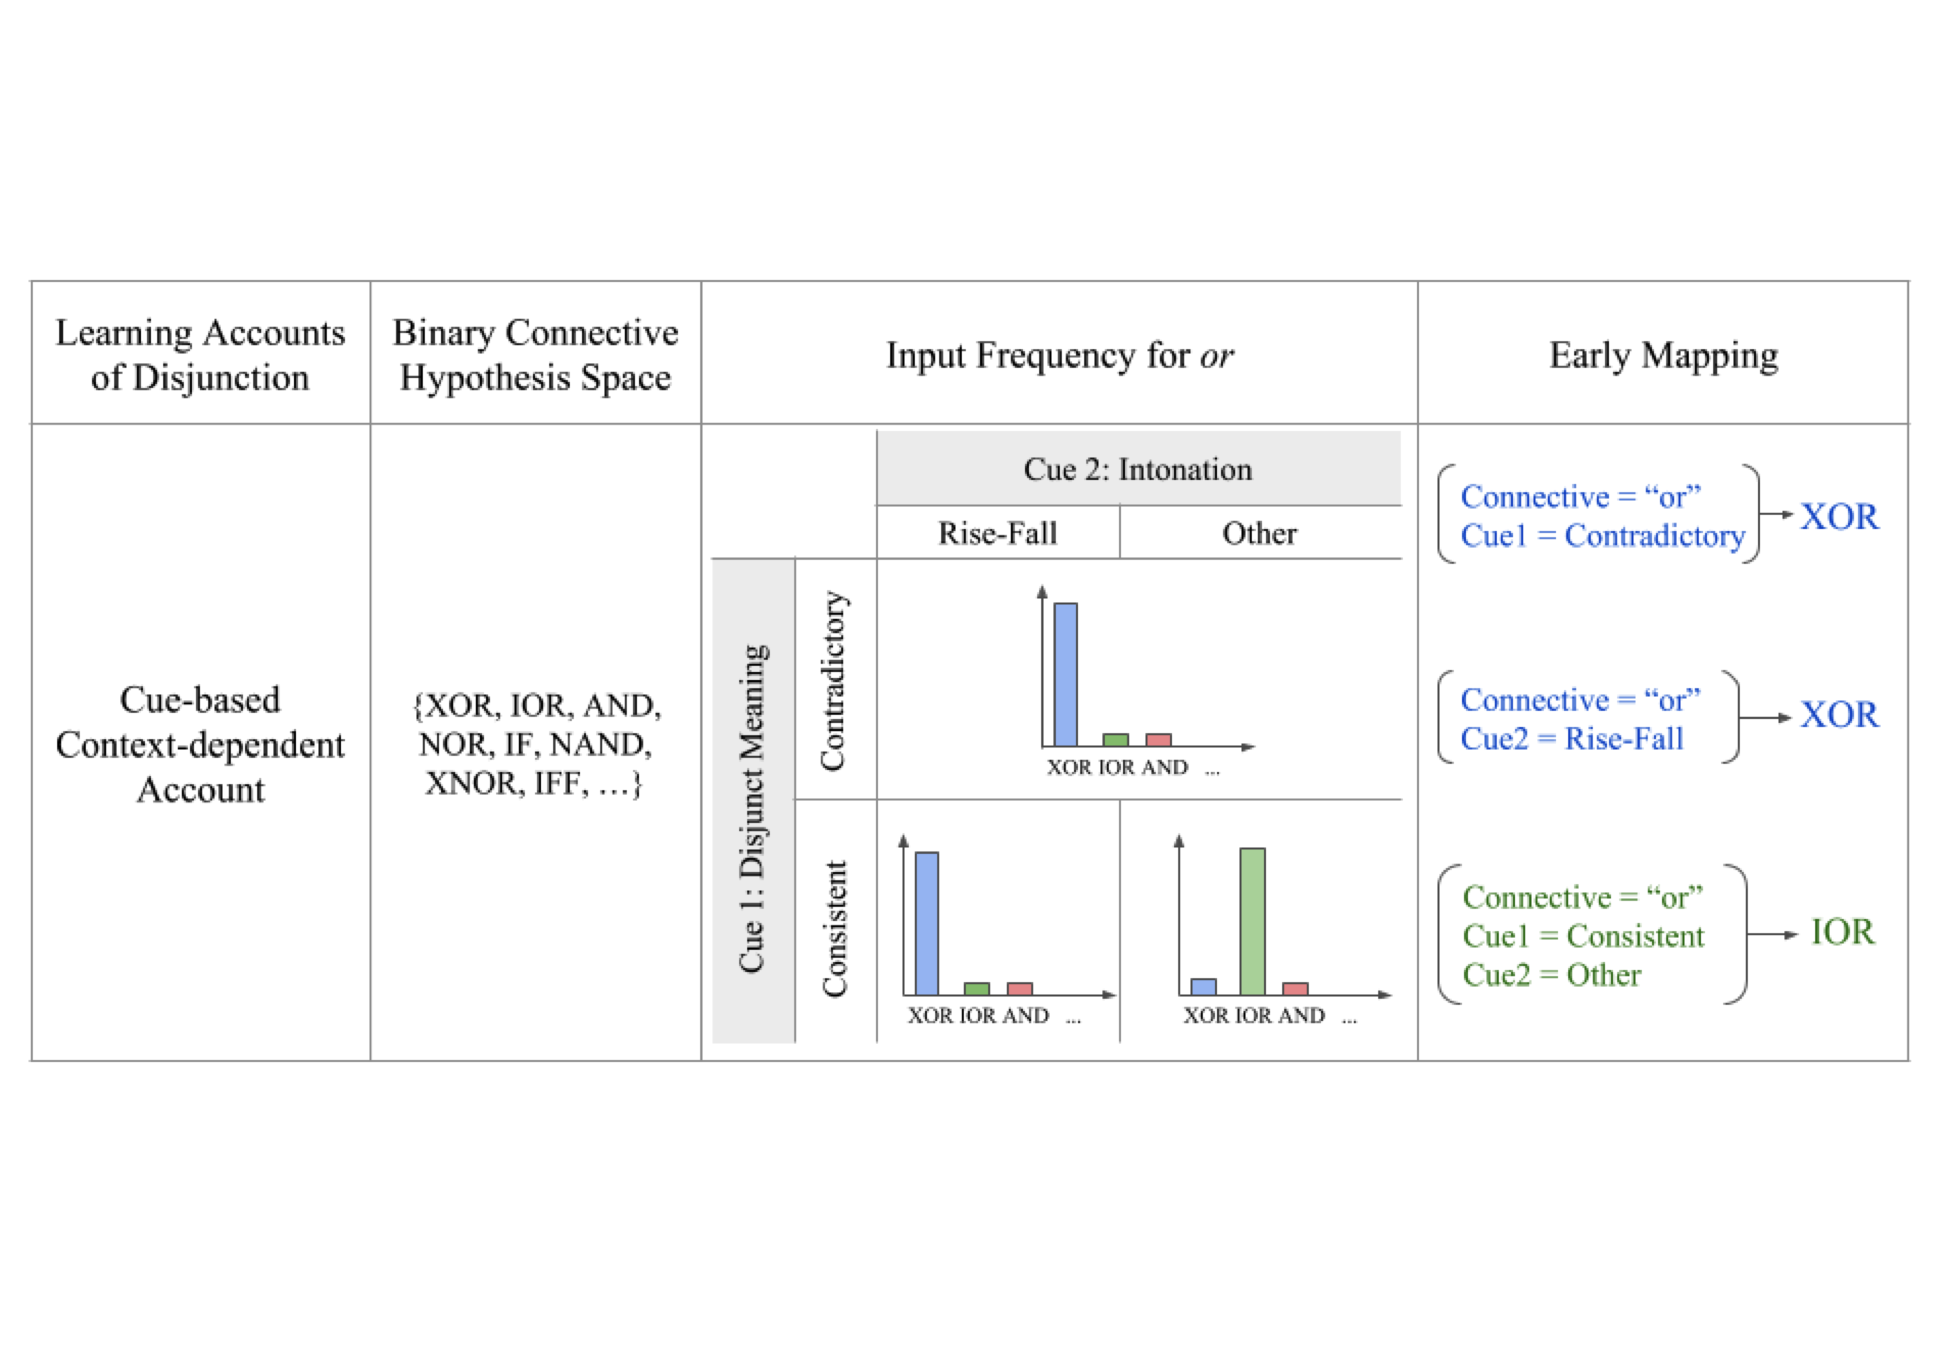
\includegraphics{figs/cueBasedAccount-1} 

}

\caption{Summary of the usage-based and nativist approaches to the acquisition of disjunction.}\label{fig:cueBasedAccount}
\end{figure}

\hypertarget{study-1-disjunction-in-adult-adult-interactions}{%
\section{Study 1: Disjunction in adult-adult interactions}\label{study-1-disjunction-in-adult-adult-interactions}}

\hypertarget{study-2-disjunction-in-parent-child-interactions}{%
\section{Study 2: Disjunction in parent-child interactions}\label{study-2-disjunction-in-parent-child-interactions}}

\hypertarget{methods}{%
\subsection{Methods}\label{methods}}

For samples of parents' and children's speech, this study used the online database \href{childes-db.stanford.edu}{childes-db} and its associated R programming package \texttt{childesr} (Sanchez et al., 2018). Childes-db is an online interface to the child language components of \href{https://talkbank.org/}{TalkBank}, namely \href{https://childes.talkbank.org/}{CHILDES} (MacWhinney, 2000) and \href{https://phonbank.talkbank.org/}{PhonBank}. Two collections of corpora were selected: English-North America and English-UK. All word tokens were tagged for the following information: 1. The speaker role (mother, father, child), 2. the age of the child when the word was produced, 3. the type of the utterance the word appeared in (declarative, question, imperative, other), and 4. whether the word was \emph{and}, \emph{or}, or neither.

\begin{figure}[tb]

{\centering 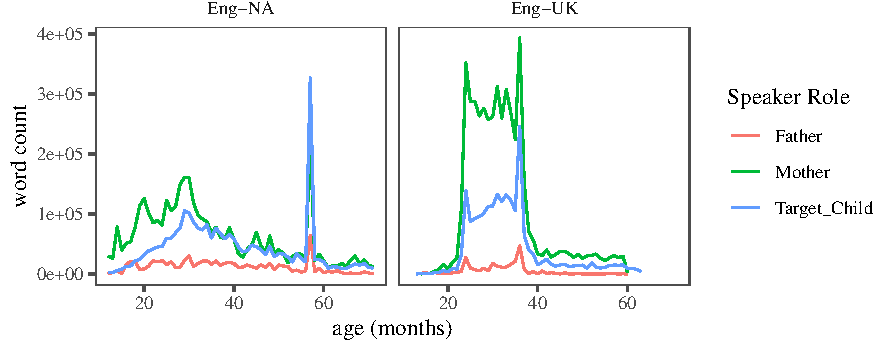
\includegraphics{figs/corpusDensityPlot-1} 

}

\caption{Frequency for all the words in the North America and UK corpora of CHILDES.}\label{fig:corpusDensityPlot}
\end{figure}

\hypertarget{exclusion-criteria}{%
\subsubsection{Exclusion Criteria}\label{exclusion-criteria}}

First, observations (tokens) that were coded as unintelligible were excluded (N = 290,119). Second, observations that had missing information on children's age were excluded (N = 1,042,478). Third, observations outside the age range of 1 to 6 years were excluded (N = 686,870). This exclusion was because we were interested in the 1 to 6 years old age range and there was not much data outside this age range either. The collection contained the speech of 504 children and their parents after the exclusions.

\hypertarget{procedure}{%
\subsubsection{Procedure}\label{procedure}}

Each token was marked for the utterance type that the token appeared in. This study grouped utterance types into four main categories: \enquote{declarative}, \enquote{question}, \enquote{imperative}, and \enquote{other}. Utterance type categorization followed the convention used in the \href{https://talkbank.org/manuals/CHAT.html\#_Toc486414422}{TalkBank manual}. The utterance types are similar to sentence types (declarative, interrogative, imperative) with one exception: the category \enquote{question} consists of interrogatives as well as rising declaratives (i.e.~declaratives with rising question intonation). In the transcripts, declaratives are marked with a period, questions with a question mark, and imperatives with an exclamation mark. It is important to note that the manual also provides \href{https://talkbank.org/manuals/CHAT.html\#_Toc486414431}{terminators for special-type utterances}. Among the special type utterances, this study included the following in the category \enquote{questions}: trailing off of a question, question with exclamation, interruption of a question, and self-interrupted question. The category imperatives also included \enquote{emphatic imperatives}. The rest of the special type utterances such as \enquote{interruptions} and \enquote{trailing off} were included in the category \enquote{other}.\\

\hypertarget{properties-of-childes-corpora}{%
\subsection{Properties of CHILDES Corpora}\label{properties-of-childes-corpora}}

In this section, I report some results on the distribution of words and utterances among the speakers in our collection of corpora. The collection contained 14,159,609 words. Table (\ref{tab:countTable}) shows the total number of \emph{and}'s, \emph{or}'s, and words in the speech of children, fathers, and mothers. The collection contains 8.80 times more words for mothers compared to fathers and 1.80 more words for mothers compared to children. Therefore, the collection is more representative of the mother-child interactions than father-child interactions. Compared to \emph{or}, the word \emph{and} is 10.80 times more likely in the speech of mothers, 9.20 times more likely in the speech of fathers, and 30.30 times more likely in the speech of children. Overall, \emph{and} is 13.35 times more likely than \emph{or} in this collection which is close to the rate reported by Morris (2008) who used a smaller subset of CHILDES. He extracted 5,994 instances of \emph{and} and 465 instances of \emph{or} and found that overall, \emph{and} was 12.89 times more frequent than \emph{or} in parent-child interactions.

\begin{table}

\caption{\label{tab:countTable}Number of \textit{and}'s, \textit{or}'s, and the total number of words in the speech of children and their parents in English-North America and English-UK collections after exclusions.}
\centering
\begin{tabular}[t]{l|r|r|r}
\hline
Speaker Role & and & or & total\\
\hline
Father & 15,488 & 1,683 & 967,075\\
\hline
Mother & 153,781 & 14,288 & 8,511,478\\
\hline
Target\_Child & 78,443 & 2,590 & 4,681,056\\
\hline
\end{tabular}
\end{table}

Figure \ref{fig:wordsByAge} shows the number of words spoken by parents and children at each month of the child's development. The words in the collection are not distributed uniformly and there is a high concentration of data between the ages of 20 and 40 months (around 2 to 3 years of age). There is also a high concentration around 60 months (5 years of age). The speech of fathers shows a relatively low word-count across all ages. Therefore, in our analyses we should be more cautious in drawing conclusions about the speech of fathers generally, and the speech of mothers and children after age 5.
The distribution of function words is sensitive to the type of utterance or more broadly the type of speech act produced by speakers. For example, it is not surprising to hear a parent say \enquote{go to your room} but a child saying the same to a parent is unexpected. If a function word commonly occurs in such speech acts, it is unlikely to be produced by children, even though they may understand it very well. Therefore, it is important to check the distribution of speech acts in corpora when studying different function words. Since it is hard to classify and quantify speech acts automatically, here I use utterance type as a proxy for speech acts. I investigate the distribution of declaratives, questions, and imperatives in this collection of corpora on parent-child interactions. Figure \ref{fig:totalUtteranceTypePlot} shows the distribution of different utterance types in the speech of parents and children. Overall, most utterances are either declaratives or questions, and there are more declaratives than questions in this collection. While mothers and fathers show similar proportions of declaratives and questions in their speech, children produce a lower proportion of questions and higher proportion of declaratives than their parents.

\begin{figure}[tb]

{\centering 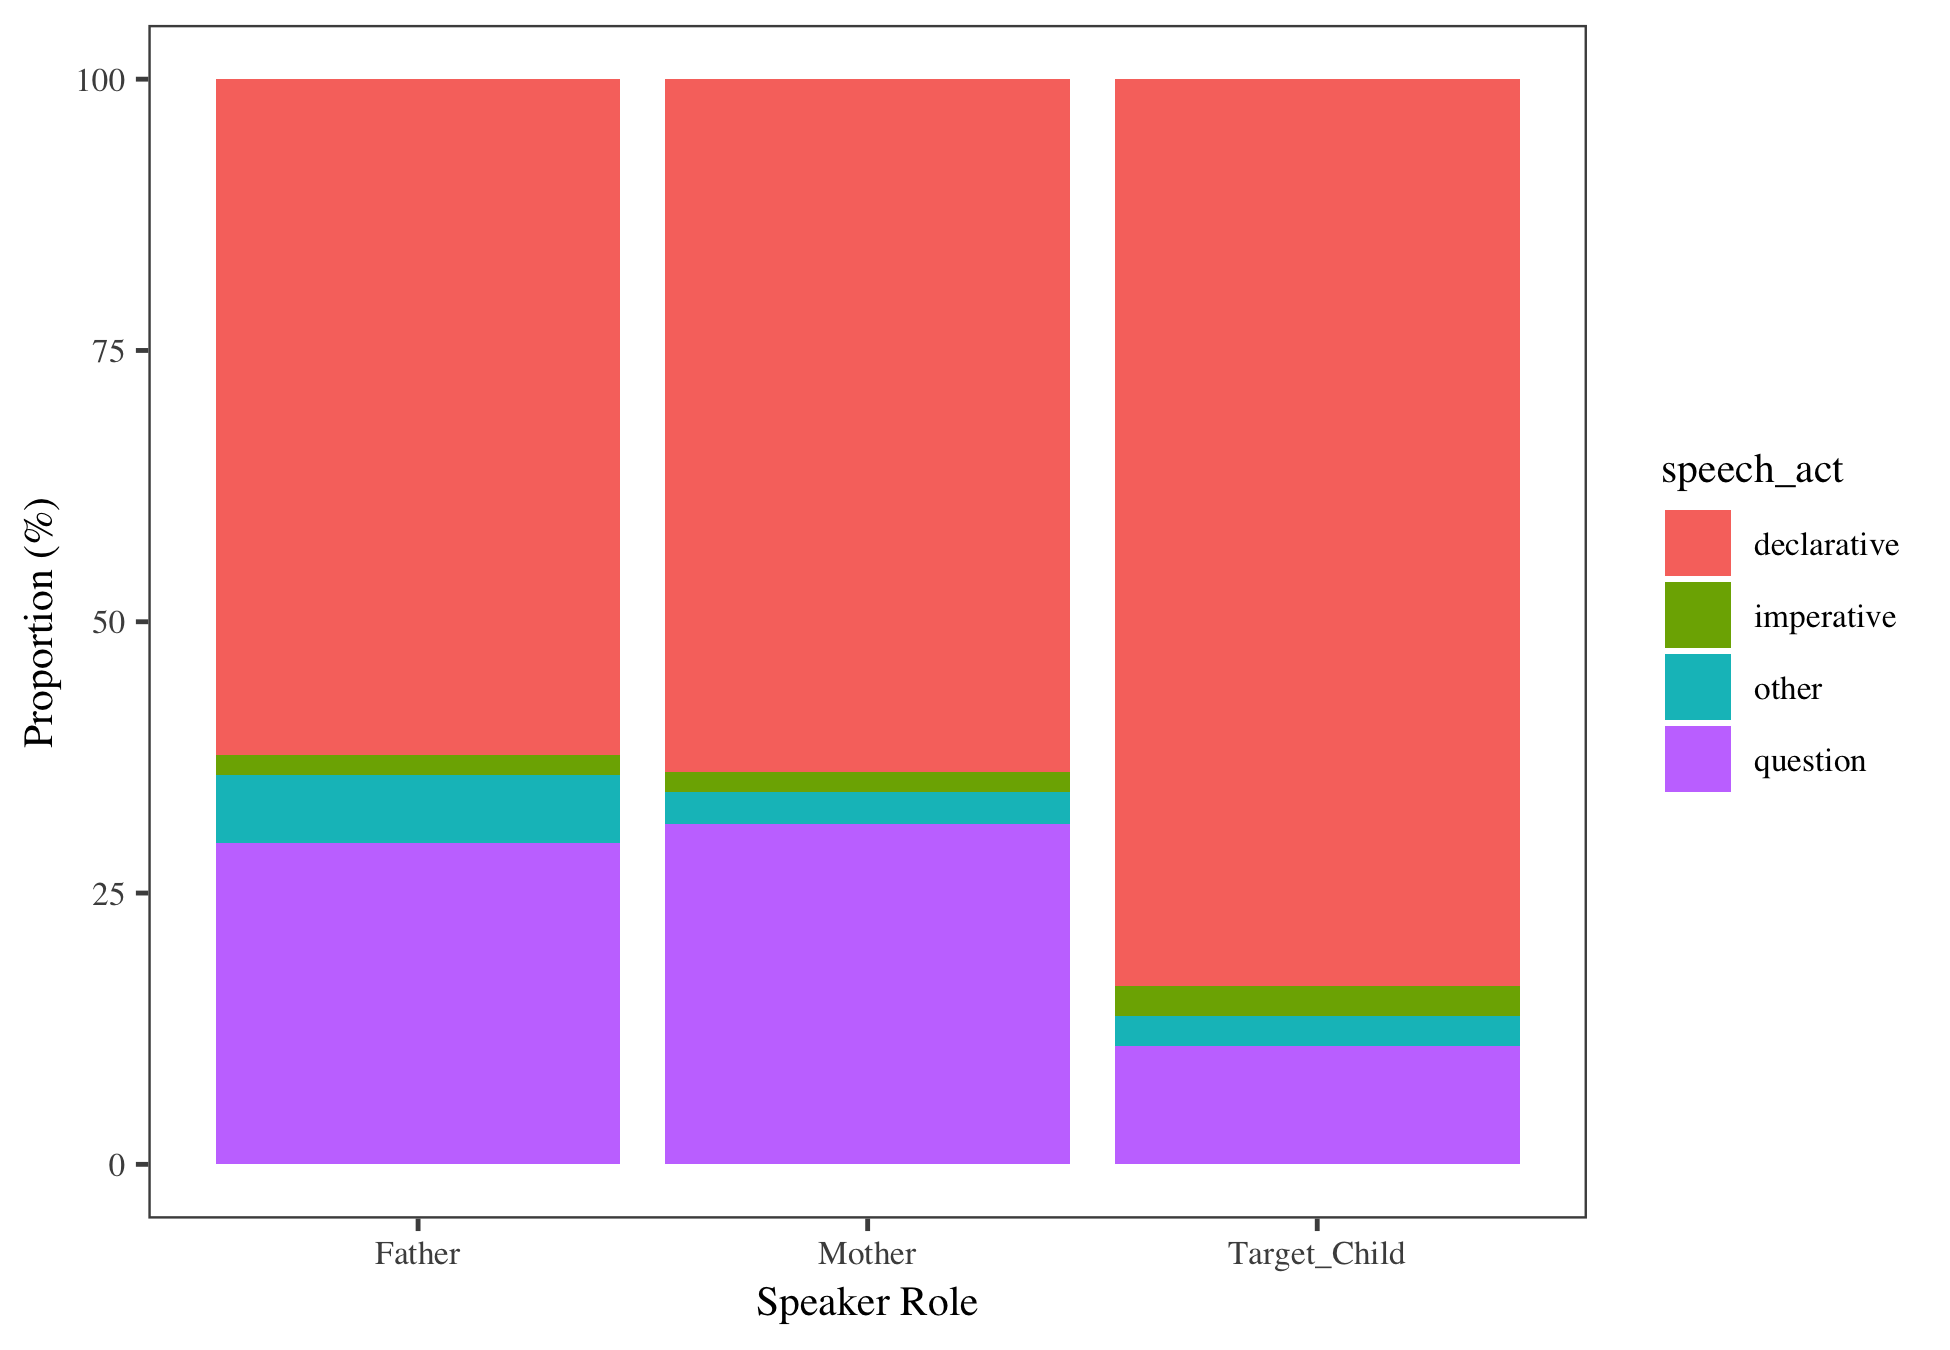
\includegraphics{figs/totalUtteranceTypePlot-1} 

}

\caption{The proportion of declaratives and questions in children's and parents' utterances.}\label{fig:totalUtteranceTypePlot}
\end{figure}

Figure \ref{fig:utteranceTypeByAgePlot} shows the developmental trend of declaratives and questions between the ages of one and six. Children start with only producing declaratives and add non-declarative utterances to their repertoire gradually until they get closer to the parents' rate around the age six. They also start with very few questions and increase the number of questions they ask gradually. It is important to note that the rates of declaratives and questions in children's speech do not reach the adult rate. These two figures show that parent-child interactions are asymmetric. Parents ask more questions and children produce more declaratives. This asymmetry also interacts with age: the speech of younger children has a higher proportion of declaratives than older children.

\begin{figure}
\centering
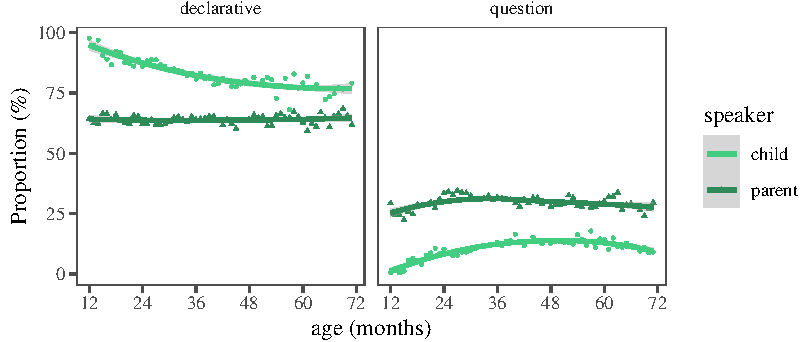
\includegraphics{figs/utteranceTypeByAgePlot-1.pdf}
\caption{\label{fig:utteranceTypeByAgePlot}Proportion of declaratives to questions in parent-child interactions by age.}
\end{figure}

The frequency of function words such as \emph{and} and \emph{or} may be affected by such conversational asymmetries if they are more likely to appear in some utterance types than others. Figure \ref{fig:CnctPropbySpeechAct} shows the proportion of \emph{and}'s and \emph{or}'s that appear in different utterance types in parents' and children's speech. In parents' speech, \emph{and} appears more often in declaratives (around 60\% in declaratives and 20\% in questions). On the other hand, \emph{or} appears more often in questions than declaratives, although this difference is small in mothers. In children's speech, both \emph{and} and \emph{or} appear most often in declaratives. However, children have a higher proportion of \emph{or} in questions than \emph{and} in questions.

The differences in the distribution of utterance types can affect our interpretation of the corpus data on function words such as \emph{and} and \emph{or} in three ways. First, since the collection contains more declaratives than questions, it may reflect the frequency and diversity of function words like \emph{and} that appear in declaratives better. Second, since children produce more declaratives and fewer questions than parents, we may underestimate children's knowledge of function words like \emph{or} that are frequent in questions. Third, given that the percentage of questions in the speech of children increases as they get older, function words like \emph{or} that are more likely to appear in questions may appear infrequent in the early stages and more frequent in the later stages of children's development. In other words, function words like \emph{or} that are common in questions may show a seeming delay in production which is possibly due to the development of questions in children's speech. Therefore, in studying children's productions of function words, it is important to look at their relative frequencies in different utterance types as well as the overall trends. This is the approach I pursue in the next section.

\begin{figure}[tb]

{\centering 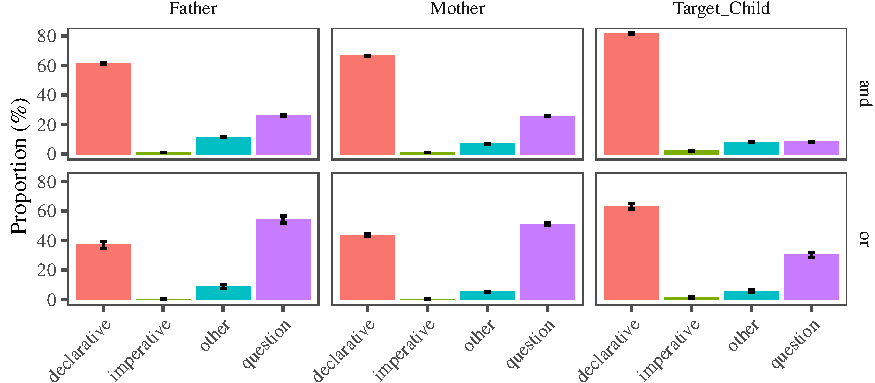
\includegraphics{figs/CnctPropbySpeechAct-1} 

}

\caption{The proportion of \textit{and} and \textit{or} in different utterance types in the speech of parents and children.}\label{fig:CnctPropbySpeechAct}
\end{figure}

\hypertarget{study1results}{%
\subsection{Results}\label{study1results}}

First, I consider the overall distribution of \emph{and} and \emph{or} in the corpora and then look closer at their distributions in different utterance types. Figure \ref{fig:freqTableBySpeakerPlot} shows the frequency of \emph{and} and \emph{or} relative to the total number of words produced by each speaker (i.e.~fathers, mothers, and children). The y-axes show relative frequency per thousand words. It is also important to note that the y-axes show different ranges of values for \emph{and} vs. \emph{or}. This is due to the large difference between the relative frequencies of these connectives. Overall, \emph{and} occurs around 15 times per thousand words but \emph{or} only occurs 3 times per 2000 words in the speech of parents and around 1 time every 2000 words in the speech of children. Comparing the relative frequency of the connectives in parents' and children's speech, we can see that overall, children and parents produce similar rates of \emph{and} in their interactions. However, children produce fewer \emph{or}'s than their parents.

\begin{figure}[tb]

{\centering 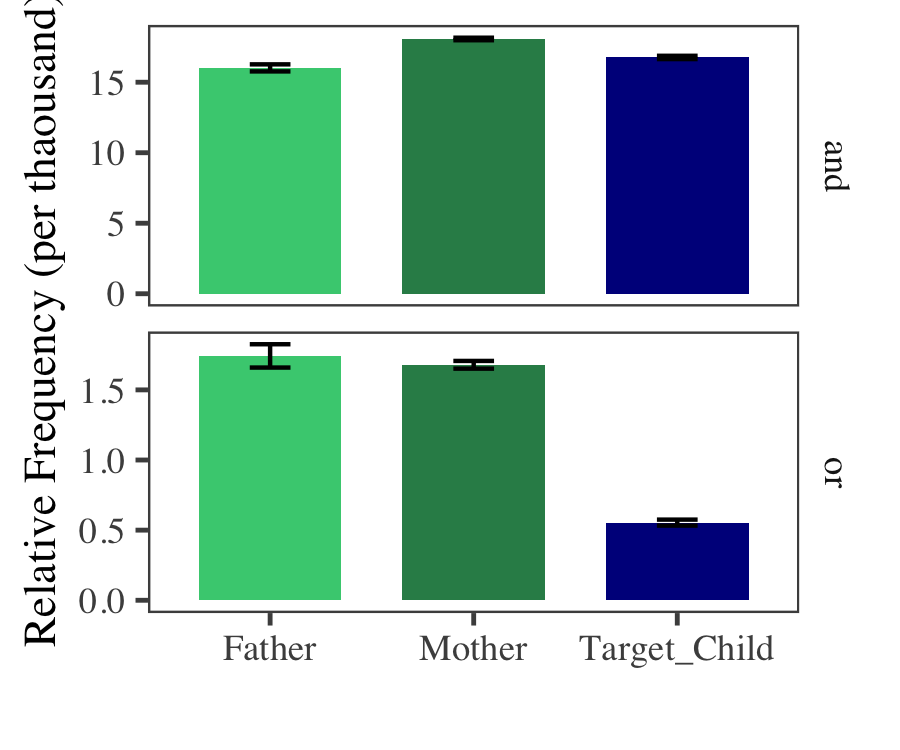
\includegraphics{figs/freqTableBySpeakerPlot-1} 

}

\caption{The relative frequency of \textit{and/or} in the speech of fathers, mothers, and children. 95\% binomial proportion confidence intervals calculated using Agresti-Coull's approximate method.}\label{fig:freqTableBySpeakerPlot}
\end{figure}

Next we look at the relative frequencies of \emph{and} and \emph{or} in parents and children's speech during the course of children's development. Figure \ref{fig:agePlot} shows the relative frequencies of \emph{and} and \emph{or} in parents' and children's speech between 12 and 72 months (1-6 years). Production of \emph{and} in parents' speech seems to be relatively stable and somewhere between 10 to 20 \emph{and}'s per thousand words over the course of children's development. For children, they start producing \emph{and} between 12 and 24 months, and show a sharp increase in their production until they reach the parent level between 30 to 36 months of age. Children stay close to the parents' production level between 36 and 72 months, possibly surpassing them a bit at 60 months -- although as stated in the previous section, we should be cautious about patterns after 60 months due to the small amount of data in this period. For \emph{or}, parents produce between 1 to 2 \emph{or}'s every thousand words and mothers show a slight increase in their productions between 12 to 36 months. Children start producing \emph{or} between 18 to 30 months of age. They show a steady increase in their productions of \emph{or} until they get close to 1 \emph{or} per thousand words at 48 months (4 years) and stay at that level until 72 months (6 years).

Children's productions of \emph{and} and \emph{or} show two main differences. First, the onset of \emph{or} production is later than that of \emph{and}. Children start producing \emph{and} around 1 to 1.5 years old while \emph{or} productions start around 6 months later. Second, children's \emph{and} production shows a steep rise and reaches the parent level of production at three-years old. For \emph{or}, however, the rise in children's production level does not reach the parent level even though it seems to reach a constant level between the ages of 4 and 6 years.

Not reaching the parent level of \emph{or} production does not necessarily mean that children's understanding of \emph{or} has not fully developed yet. It can also be due to the nature of parent-child interactions. For example, since parents ask more questions than children and \emph{or} appears frequently in questions, parents may have a higher frequency of \emph{or}. There are two ways of controlling for this possibility. One is to research children's speech to peers. Unfortunately such a large database of children's speech to peers is not currently available for analysis. Alternatively, we can look at the relative frequencies and developmental trends within utterance types such as declaratives and questions to see if we spot different developmental trends. This is what I pursue next.

\begin{figure}[tb]

{\centering 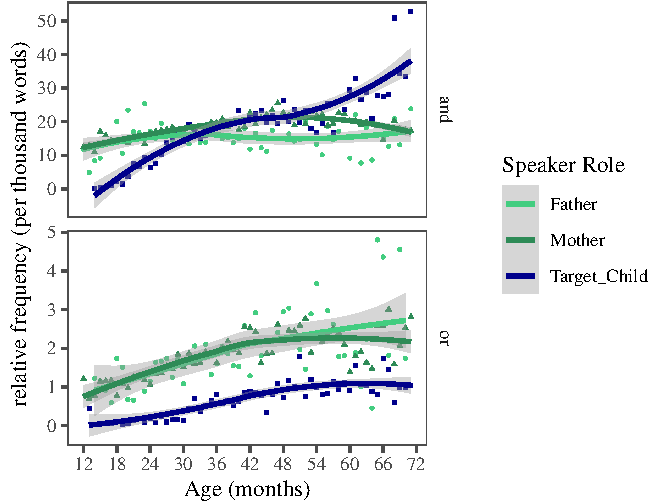
\includegraphics{figs/agePlot-1} 

}

\caption{The monthly relative frequency of \textit{and/or} in parents and children's speech between 12 and 72 months (1-6 years).}\label{fig:agePlot}
\end{figure}

Figure \ref{fig:freqTablebySpeechAct} shows the relative frequency of \emph{and} and \emph{or} in declaratives, questions, and imperatives. \emph{And} has the highest relative frequency in declaratives while \emph{or} has the highest relative frequency in questions. Figure \ref{fig:ageSpeechActPlot} shows the developmental trends of the relative frequencies of \emph{and} and \emph{or} in questions and declaratives. Comparing \emph{and} in declaratives and questions, we see that the onset of \emph{and} productions are slightly delayed for questions but in both declaratives and questions, \emph{and} productions reach the parent level around 36 months (3 years). For \emph{or}, we see a similar delay in questions compared to declaratives. Children start producing \emph{or} in declaratives at around 18 months but they start producing \emph{or} in questions at 24 months. Production of \emph{or} increases in both declaratives and questions until it seems to reach a constant rate in declaratives between 48 and 72 months. The relative frequency of \emph{or} in questions continues to rise until 60 months. Comparing figures \ref{fig:agePlot} and \ref{fig:ageSpeechActPlot}, we see that children are closer to the adult rate of production in declaratives than questions. The large difference between parents and children's production of \emph{or} in figure \ref{fig:agePlot} may partly be due to the development of \emph{or} in questions. Overall the results show that children have a substantial increase in their productions of \emph{and} and \emph{or} between 1.5 to 4 years of age. Therefore, it is reasonable to expect that early mappings for the meaning and usage of these words develop in this age range.

\begin{figure}[tb]

{\centering 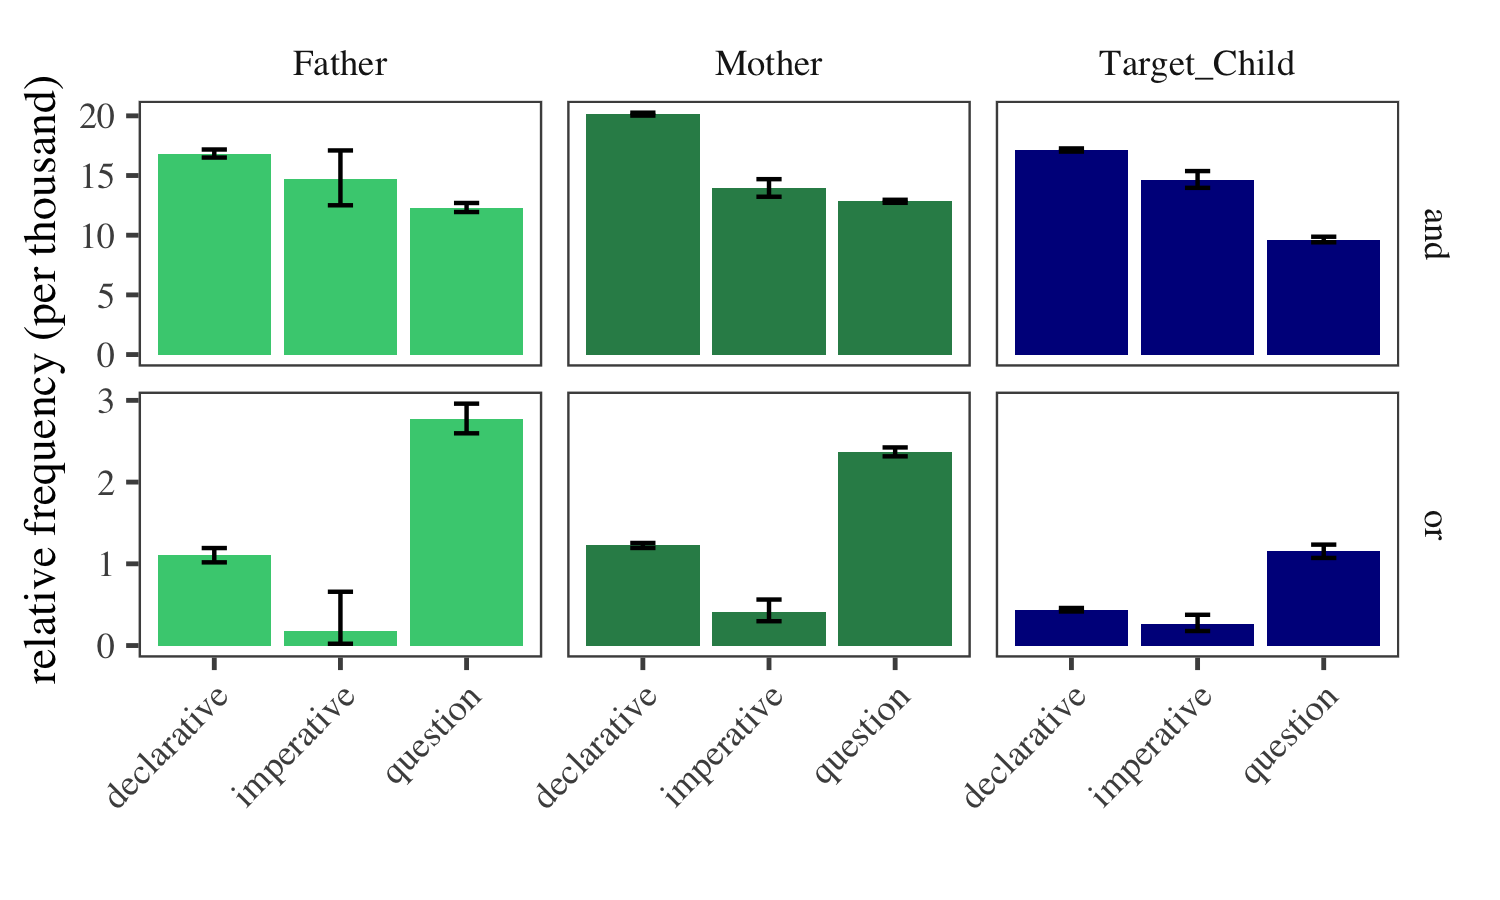
\includegraphics{figs/freqTablebySpeechAct-1} 

}

\caption{Relative frequency of \textit{and/or} in declaratives, imperatives, and interrogatives for parents and children }\label{fig:freqTablebySpeechAct}
\end{figure}

\begin{figure}[tb]

{\centering 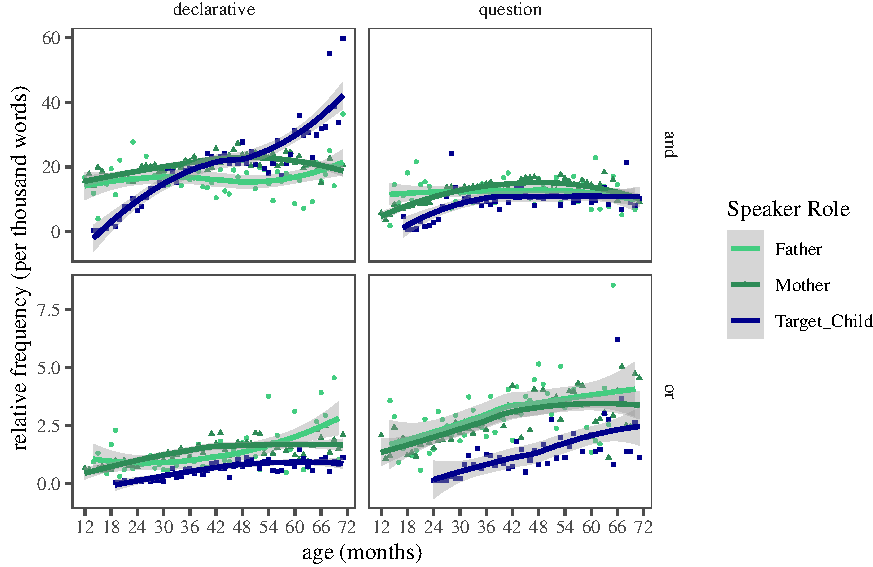
\includegraphics{figs/ageSpeechActPlot-1} 

}

\caption{Relative frequency of \textit{and/or} in declaratives and questions for parents and childern between the child-age of 12 and 72 months (1-6 years).}\label{fig:ageSpeechActPlot}
\end{figure}

\hypertarget{study1discussion}{%
\subsection{Discussion}\label{study1discussion}}

The goal of this study was to explore the frequency of \emph{and} and \emph{or} in parents and children's speech. The study found three differences. First, it found a difference between the overall frequency of \emph{and} and \emph{or} in both parents and children. \emph{And} was about 10 times more frequent than \emph{or} in the speech of parents and 30 times more likely in the speech of children. Second, the study found a difference between parents' and children's productions of \emph{or}. Relative to the total number of words spoken by parents and children between the ages of 1 and 6 years, both children and parents produce on average 15 \emph{and}'s every 1000 words. Therefore, children match parents' rate of \emph{and} production overall. This is not the case for \emph{or} as parents produce 3 \emph{or}'s every 2000 words and children only 1 every 2000 words. Third, the study found a developmental difference between \emph{and} and \emph{or} as well. The study found that the onset of production is earlier for \emph{and} than \emph{or}. In the monthly relative frequencies of \emph{and} and \emph{or} in the speech of parents and children, the study also found that children reach the parents' level of production for \emph{and} at age 3 while \emph{or} does not reach the parents' level even at age 6.

What causes these production differences? The first difference -- that \emph{and} is far more frequent than \emph{or} -- is not surprising or limited to child-directed speech. \emph{And} is useful in a large set of contexts from conjoining elements of a sentence to connecting discourse elements or even holding the floor and delaying a conversational turn. In comparison, \emph{or} seems to have a more limited usage. The second and the third differences -- namely that children produce fewer \emph{or}'s than parents, and that they produce \emph{and} and reach their parents rate earlier than \emph{or} -- could be due to three factors. First, production of \emph{and} develops and reaches the parents' rate earlier possibly because it is much more frequent than \emph{or} in children's input. Previous research suggests that within the same syntactic category, words with higher frequency in child-directed speech are acquired earlier (Goodman, Dale, \& Li, 2008). The conjunction word \emph{and} is at least 10 times more likely than \emph{or} so earlier acquisition of \emph{and} is consistent with the effect of frequency on age of acquisition. Second, research on concept attainment has suggested that the concept of conjunction is easier to conjure and possibly acquire than the concept of disjunction. In experiments that participants are asked to detect a pattern in the classification of cards, participants can detect a conjunctive classification pattern faster than a disjunctive one (Neisser \& Weene, 1962). Therefore, it is possible that children learn the meaning of \emph{and} faster and start to produce it earlier but they need more time to figure out the meaning and usage of \emph{or}.

A third possibility is that the developmental difference between \emph{and} and \emph{or} is mainly due to the asymmetric nature of parent-child interactions and the utterance types that each role in this interaction requires. For example, this study found that parents ask more questions of children than children do of parents. It also found that \emph{or} is much more frequent in questions than \emph{and} is. Therefore, parent-child interaction provides more opportunities for parents to use \emph{or} than children. In the next study we will discuss several constructions and communicative functions that are also more appropriate for the role of parents. For example, \emph{or} is often used to ask what someone else wants like \enquote{do you want apple juice or orange juice?} or for asking someone to clarify what they said such as \enquote{did you mean ball or bowl?}. Both of these constructions are more likely to be produced by a parent than a child. \emph{Or} is also used to introduce examples or provide definitions such as \enquote{an animal, like a rabbit, or a lion, or a sheep}. It is very unlikely that children would use such constructions to define terms for parents! Furthermore, such constructions also reveal their own developmental trends. For example, the study found that children start by almost entirely producing declaratives and increase their questions until at age 4 to 6, about 10\% of their utterances are questions. Therefore, children's ability to produce \emph{or} in a question is subject to the development of questions themselves. More generally, the developmental difference between \emph{and} and \emph{or} may also be due to a difference in the development of other factors that production of \emph{and} and \emph{or} rely on, such as the development of constructions with specific communicative functions like unconditionals (Whether X or Y, discussed in Chapter \ref{sempragLit}). In future research, it will be important to establish the extent to which each of these potential causes -- frequency, conceptual complexity, and the development of other factors such as utterance type or constructions with specific communicative functions -- contribute to the developmental differences in the production of conjunction and disjunction.

\hypertarget{study-3-interpretations-of-disjunction-in-child-directed-speech}{%
\section{Study 3: Interpretations of disjunction in child-directed speech}\label{study-3-interpretations-of-disjunction-in-child-directed-speech}}

Previous study reported on the frequencies of disjunction in parents and children's speech production. To help us better understand children's linguistic input, this study offers a close examination of the interpretations that \emph{and} and \emph{or} have in child-directed speech. It had two main goals. First, to replicate the finding of Morris (2008) and second, to identify any cues in children's input that might help them learn the interpretations of disjunction in English.

\hypertarget{methods-1}{%
\subsection{Methods}\label{methods-1}}

This study used \href{https://phonbank.talkbank.org/browser/index.php?url=Eng-NA/Providence/}{the Providence corpus} (Demuth, Culbertson, \& Alter, 2006) available via the \href{https://phonbank.talkbank.org}{PhonBank} section of \href{https://talkbank.org/}{the TalkBank.org archive}. The corpus was chosen because of its relatively dense data on child-directed speech as well as the availability of audio and video recordings that would allow annotators access to the context of the utterance. The corpus was collected between 2002 and 2005 in Providence, Rhode Island. Table \ref{tab:providence} reports the name, age range, and the number of recording sessions for the participants in the study. All children were monolingual English speakers and were followed between the ages of 1 and 4 years. Based on Study 2, this is the age range when children develop their early understanding or mappings for the meanings of \emph{and} and \emph{or}. The corpus contains roughly biweekly hour-long recordings of spontaneous parent-child interactions, with most recordings being of mother-child interactions. The corpus consists of a total of 364 hours of speech.

\begin{longtable}[]{@{}ccc@{}}
\caption{\label{tab:providence} Information on the participants in the Providence Corpus. Ethan was diagnosed with Asperger's syndrome and therefore was excluded from this study.}\tabularnewline
\toprule
Name & Age Range & Sessions\tabularnewline
\midrule
\endfirsthead
\toprule
Name & Age Range & Sessions\tabularnewline
\midrule
\endhead
Alex & 1;04.28-3;05.16 & 51\tabularnewline
Ethan & 0;11.04-2;11.01 & 50\tabularnewline
Lily & 1;01.02-4;00.02 & 80\tabularnewline
Naima & 0;11.27-3;10.10 & 88\tabularnewline
Violet & 1;02.00-3;11.24 & 51\tabularnewline
William & 1;04.12-3;04.18 & 44\tabularnewline
\bottomrule
\end{longtable}

\#\#\#Exclusion Criteria
We excluded data from Ethan since he was diagnosed with Asperger's Syndrome at age 5. We also excluded all examples found in conversations over the phone, adult-adult conversations, and utterances heard from TV or radio. We did not count such utterances as child-directed speech. We excluded proper names and fixed forms such as \enquote{Bread and Circus} (name of a local place) or \enquote{trick-or-treat} from the set of examples to be annotated. The rationale here was that such forms could be learned and understood with no actual understanding of the connective meaning. We counted multiple instances of \emph{or} and \emph{and} within the same disjunction/conjunction as one instance. The reasoning was that, in a coordinated structure, the additional occurrences of a connective typically did not alter the annotation categories, and most importantly the interpretation of the coordination. For example, there is almost no difference between \enquote{cat, dog, and elephant} versus \enquote{cat and dog and elephant} in interpretation. In short, we focused on the \enquote{coordinated construction} as a unit rather than on every separate instance of \emph{and} and \emph{or}. Instances of multiple connectives in a coordination were rare in the corpus.

\#\#\#Procedure
All utterances containing \emph{and} and \emph{or} were extracted using \href{http://alpha.talkbank.org/clan/}{the CLAN software} and automatically tagged for the following: (1) the name of the child; (2) the transcript address; (3) the speaker of the utterance (father, mother, or child); (4) the child's birth date, and (5) the recording date. Since the focus of the study was mainly on disjunction, we annotated instances of \emph{or} in all the child-directed speech from the earliest examples to the latest ones found. Given that the corpus contained more than 10 times the number of \emph{and}'s than \emph{or}'s, we randomly sampled 1000 examples of \emph{and} to match 1000 examples of \emph{or}. Here we report the results on 465 examples of \emph{and} and 608 examples of \emph{or}.

\hypertarget{annotation-categories}{%
\subsubsection{Annotation Categories}\label{annotation-categories}}

Every extracted instance of \emph{and} and \emph{or} was manually annotated for 7 categories: 1. Connective Interpretation 2. Intonation Type 3. Utterance Type 4. Syntactic Level 5. Conceptual Consistency 6. Communicative Function and 7. Answer Type. In what follows, I briefly explain how each annotation category was defined. Further details and examples are provided in the appendix section.

\hypertarget{connective-interpretation}{%
\paragraph{Connective Interpretation}\label{connective-interpretation}}

This annotation category was the dependent variable of the study. Annotators listened to coordinations such as \enquote{A or B} and \enquote{A and B}, and decided the intended interpretation of the connective with respect to the truth of A and B. We used the sixteen binary connectives shown in Figure \ref{fig:logicalConnectives} as the space of possible connective interpretations. Annotators were asked to consider the two propositions raised by the coordinated construction, ignoring the connective and functional elements such as negation and modals. Consider the following sentences containing \emph{or}: \enquote{Bob plays soccer or tennis} and \enquote{Bob doesn't play soccer or tennis}. Both discuss the same two propositions: A. Bob playing soccer, and B. Bob playing tennis. However, the functional elements combining these two propositions result in different interpretations with respect to the truth of A and B. In \enquote{Bob plays soccer or tennis} which contains a disjunction, the interpretation is that Bob plays one or possibly both sports (inclusive disjunction IOR). In \enquote{Bob doesn't play soccer or tennis} which contains a negation and a disjunction, the interpretation is that Bob plays neither sport (NOR). For connective interpretations, the annotators first reconstructed the coordinated propositions without the connectives or negation and then decided which propositions were implied to be true/false.

This approach is partly informed by children's development of function and content words. Since children acquire content words earlier than functions words, we assumed that when learning logical connectives, they better understand the content of the propositions being coordinated rather than the functional elements involved in building the coordinated construction. For example, considering the sentences \enquote{Bob doesn't play soccer or tennis} without its function words as \enquote{Bob, play, soccer, tennis}, one can still deduce that there are two relevant propositions: Bob playing soccer, and Bob playing tennis. However, the real challenge is to figure out what is being communicated with respect to the truth of these two propositions. If the learner can figure this out, then the meaning of the functional elements can be reverse engineered. For example, if the learner recognizes that \enquote{Bob plays soccer or tennis} communicates that one or both propositions are true (IOR), the learner can associate this interpretation to the unknown element \emph{or}. Similarly, if the learner recognizes the interpretation of \enquote{Bob doesn't play soccer or tennis} as neither proposition is true (NOR), they can associate this interpretation to the co-presence of \emph{or} and \emph{doesn't}. Table \ref{tab:connectiveInterpretaion} in the appendix section reports the connective interpretations found in our annotations as well as some examples for each interpretation.

\#\#\#\#Intonation Type
Annotators listened to the utterances and decided whether the intonation contour on the coordination was flat, rise, or rise-fall. Table \ref{tab:intonationTypes} in the appendix shows the definitions and examples for these intonation types. In order to judge the intonation of the sentence accurately, annotators were asked to construct all three intonation contours for the sentence and see which one is closer to the actual intonation of the utterance. For example, to judge the sentence \enquote{do you want orange juice\(\uparrow\) or apple juice\(\downarrow\)?}, they reconstructed the sentence with the prototypical flat, rising, and rise-fall intonations and checked to see which intonation is closer to the actual one. It is important to note that while these three intonation contours provide a good general classification, there is a substantial degree of variation as well as a good number of subtypes within each intonation type.

\#\#\#\#Utterance Type
Annotators decided whether an utterance was an instance of a declarative, an interrogative, or an imperative. Occasionally, we found examples with different utterance types for each coordinand. For example, the mother would say \enquote{put your backpack on and I'll be right back}, where the first cooridnand is an imperative and the second a declarative. Such examples were coded for both utterance types with a dash inbetween: imperative-declarative. Table \ref{tab:utteranceTypes} in the appendix provides the definitions and examples for each utterance type.

\#\#\#\#Syntactic Level
For this annotation category, annotators decided whether the coordination was at the clausal level or at the sub-clausal level. Clausal level was defined as sentences, clauses, verb phrases, and verbs. Coordination of other categories was coded as sub-clausal. This annotation category was introduced to check the hypothesis that the syntactic category of the coordinands may influence the interpretation of a coordination. The intuition was that a sentence such as \enquote{He drank tea or coffee} is less likely to be interpreted as exclusive than \enquote{He drank tea or he drank coffee.} The clausal vs.~sub-clausal distinction was inspired by the fact that in many languages, coordinators that connect sentences and verb phrases are different lexical items than those that connect nominal, adjectival, or prepositional phrases (see Haspelmath, 2007).

\#\#\#\#Conceptual Consistency
Propositions that are connected by words such as \emph{and} and \emph{or} often stand in complex conceptual relations with each other. For conceptual consistency, annotators decided whether the propositions that make up the coordination can be true at the same time or not. If the two propositions could be true at the same time they were marked as consistent. If the two propositions could not be true at the same time and resulted in a contradiction, they were marked as inconsistent. Our annotators used the following diagnostic to decide the consistency of the disjuncts: Two disjuncts were marked as inconsistent if replacing the word \emph{or} with \emph{and} produced a contradiction. For example, changing \enquote{the ball is in my room \emph{or} your room} to \enquote{the ball is in my room \emph{and} your room} produces a contradiction because a ball cannot be in two rooms at the same time\footnote{This criterion is quite strict. In many cases, the possibility of both propositions being true is ruled out based on prior knowledge and expectations of the situation. For example, when asking people whether they would like tea or coffee, it is often assumed and expected that people choose one or the other. However, wanting to drink both tea and coffee is not conceptually inconsistent. It is just very unlikely. Our annotations of consistency are very conservative in that they still consider such unlikely cases as consistent. Relaxing this criterion to capture the unlikely cases may increase exclusivity inferences that are caused by alternatives that are considered unlikely to co-occur.
  It is also important to note that if the coordinands are inconsistent, this does not necessarily means that the connective interpretation must be exclusive. For example, in a sentence like \enquote{you could stay here or go out}, the alternatives \enquote{staying here} and \enquote{going out} are inconsistent. Yet, the overall interpretation of the connective could be conjunctive: you could stay here AND you could go out. The statement communicates that both possibilities hold. This pattern of interaction between possibility modals like \emph{can} and disjunction words like \emph{or} are often discussed under the label \enquote{free-choice inferences} in the semantics and pragmatics literature (Kamp, 1973; Von Wright, 1968). Another example is unconditionals such as \enquote{Ready or not, here I come!}. The coordinands are contradictions: one is the negation of the other. However, the overall interpretation of the sentences is that in both cases, the speaker is going to come.}.

\#\#\#\#Communicative Functions
This study constructed a set of categories that captured particular usages or communicative functions of the words \emph{or} and \emph{and}. They include descriptions, directives, preferences, identifications, definitions and examples, clarifications, repairs, and a few others shown with examples in Table \ref{tab:speechActs} in the appendix section. These communicative functions were created using the first 100 examples and then they were used for the classification of the rest of the examples. Some communicative functions are general and some are specific to coordination. For example, directives are a general class while conditionals (e.g.~Put that out of your mouth, or I'm gonna put it away) are more specific to coordinated constructions. It is also important to note that the list is not unstructured. Some communicative functions are subtypes of others. For example, \enquote{identifications} and \enquote{unconditionals} are subtypes of \enquote{descriptions} while \enquote{conditionals} are a subtype of directives. Furthermore, \enquote{repairs} seem parallel to other categories in that any type of speech can be repaired. We do not fully explore the details of these functions in this study but such details matter for a general theory of acquisition that makes use of the speaker's communicative intentions as early coarse-grained communicative cues for the acquisition of fine-grained meaning such as function words.

\#\#\#\#Answer Type
Whenever a parent's utterance was a polar question, the annotators coded the utterance for the type of response it received from the children. Table \ref{tab:answerTypes} in the appendix shows the answer types in this study and their definitions and examples. Utterances that were not polar questions were simply coded as NA for this category. If children responded to polar questions with \enquote{yes} or \enquote{no}, the category was YN and if they repeated with one of the coordinands the category was AB. If children said yes/no and followed it with one of the coordinands, the answer type was determined as YN (yes/no). For example, if a child was asked \enquote{Do you want orange juice or apple juice?} and the child responded with \enquote{yes, apple juice}, our annotators coded the response as YN. The reason is that in almost all cases, if a simple yes/no response is felicitous, then it can also be optionally followed with mentioning a disjunct. However, if yes/no is not a felicitous response, then mentioning one of the alternatives is the only appropriate answer. For example, if someone asks \enquote{Do you want to stay here or go out?} a response such as \enquote{yes, go out} is infelicitous and a better response is to simply say \enquote{go out}. Therefore, we counted responses with both yes/no and mentioning an alternative as a yes/no response.

\hypertarget{inter-annotator-reliability}{%
\subsubsection{Inter-annotator Reliability}\label{inter-annotator-reliability}}

To train annotators and confirm their reliability for disjunction examples, two annotators coded the same 240 instances of disjunction. The inter-annotator reliability was calculated over 8 iterations of 30 examples each. After each iteration, annotators met to discuss disagreements and resolve them. They also decided whether the category definitions or annotation criteria needed to be made more precise. Training was completed after three consecutive iterations showed substantial agreement between the annotators for all categories (Cohen's \(\kappa > 0.7\)). Further details on inter-annotator reliability are presented in the appendix section.

\hypertarget{results}{%
\subsubsection{Results}\label{results}}

First we look at how children responded to their parents' questions with \emph{or} (Answer Type). Figure \ref{fig:answerPlot} shows the monthly proportions of \enquote{yes/no} and alternative (AB) answers between the ages of 1 and 3 years. Initially, children provided no answer to questions, but by the age of 3 years, the majority of such questions received a yes/no (YN) or alternative (AB) answer. This increase in the proportion of responses to questions containing \emph{or} between 20 to 30 months of age suggests that initial form-meaning mappings for disjunction is formed in this age range.

\begin{figure}[tb]

{\centering 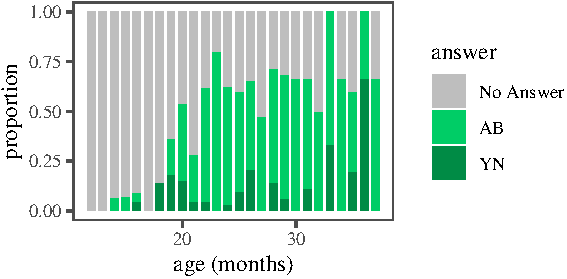
\includegraphics{figs/answerPlot-1} 

}

\caption{The proportions of children's answer types to polar questions containing the connective \textit{or} at different ages (in months).}\label{fig:answerPlot}
\end{figure}

Next we consider the interpretations that \emph{and} and \emph{or} received in child-directed speech. The most common interpretation was the conjunctive interpretation (AND, 49\%) followed by the exclusive interpretation (XOR, 35\%). Figure \ref{fig:connectivePlot} shows the distribution of connective interpretations by the connective words \emph{and} and \emph{or}\footnote{All the confidence intervals shown in the plots for this section are simultaneous multinomial confidence intervals computed using the Sison and Glaz (1995) method.}. For \emph{and}, the most frequent interpretation (in fact almost the only interpretation), was conjunction AND. For \emph{or}, the most frequent interpretation was exclusive disjunction XOR. These results replicated the findings of Morris (2008).

\begin{figure}[tb]

{\centering 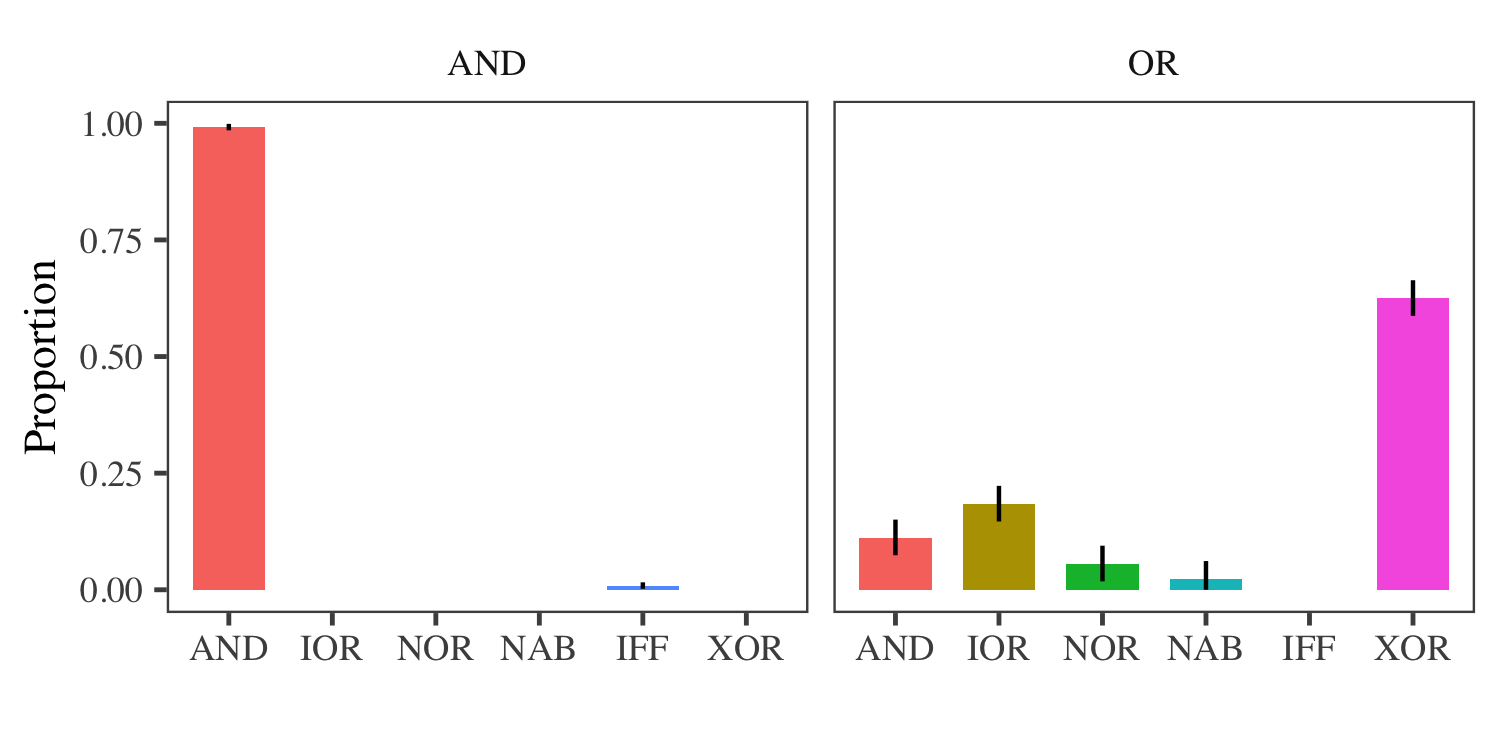
\includegraphics{figs/connectivePlot-1} 

}

\caption{Interpretations of \textit{and/or} in child-directed speech}\label{fig:connectivePlot}
\end{figure}

Morris argued that given the high frequency of conjunction and exclusive disjunction in the input, children should initially (between the ages of 2 and 5 years) map the meanings of \emph{and} and \emph{or} as conjunction and exclusive disjunction. According to Morris (2008), children learn the inclusive interpretation of disjunction later as they encounter more inclusive (logical) uses of \emph{or}. However, comprehension tasks show that children between 3 and 5 tend to interpret \emph{or} as inclusive disjunction rather than exclusive disjunction in a variety of declarative sentences (Chierchia et al., 2001; Gualmini et al., 2000a, 2000b, among others; Notley et al., 2012b). How can children learn the inclusive semantics of \emph{or} if they rarely hear it? This is the puzzle of learning disjunction, discussed in the introduction. The remainder of this section focuses on disjunction, and shows how different cues separate inclusive vs.~exclusive interpretations, which in principle can help a learner in acquiring both the inclusive and exclusive interpretations of disjunction relatively quickly.

\begin{figure}[tb]

{\centering 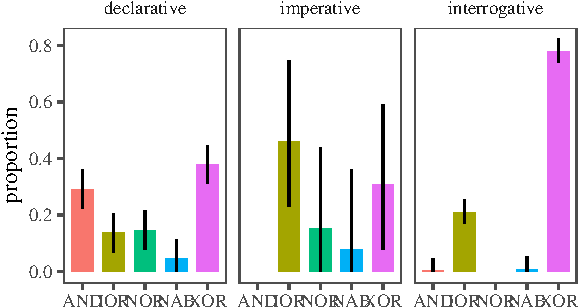
\includegraphics{figs/utterancetypePlot-1} 

}

\caption{Connective interpretations in different sentence types.}\label{fig:utterancetypePlot}
\end{figure}

Figure \ref{fig:utterancetypePlot} shows the distribution of connective interpretations in declarative, interrogative, and imperative sentences. Interrogatives select for exclusive and inclusive interpretations, but overall they are more likely to be interpreted as exclusive (XOR). Imperatives are more likely to be interpreted as inclusive (IOR) or exclusive (XOR), and declaratives are most likely exclusive (XOR) or conjunctive (AND). It is important to note here that the inclusive interpretations of imperatives are largely due to invitations to action such as \enquote{Have some food or drink!}. Such invitational imperatives seem to convey inclusivity (IOR) systematically. They are often used to give the addressee full permission with respect to both alternatives and it seems quite odd to use them to imply exclusivity (e.g. \enquote{Have some food or drink but not both!}), and they do not seem to be conjunctive either (e.g. \enquote{Have some food and have some drink!}). They rather imply that the addressee is invited to have food, drink, or both.

\begin{figure}[tb]

{\centering 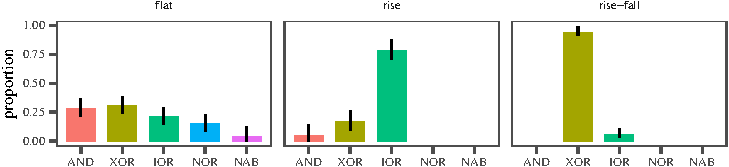
\includegraphics{figs/intonationPlot-1} 

}

\caption{The distribution of connective interpretations in flat, rising, and rise-fall intonation.}\label{fig:intonationPlot}
\end{figure}

While interrogatives select for exclusive and inclusive interpretations, their intonation can distinguish between these two readings. Figure \ref{fig:intonationPlot} shows the proportions of different connective interpretations in the three intonation contours: flat, rise, and rise-fall. The rise and rise-fall contours are typical of interrogatives. The results show that, a disjunction with a rise-fall intonation is most likely interpreted as exclusive (XOR). If the intonation is rising, a disjunction is most likely inclusive (IOR). Finally, a disjunction with a flat intonation may be interpreted as exclusive (XOR), conjunctive (AND), or inclusive (IOR). These results are consistent with Pruitt and Roelofsen (2013)'s experimental findings that a rise-fall intonation contour on a disjunction results in an exclusive interpretation.

\begin{figure}[tb]

{\centering 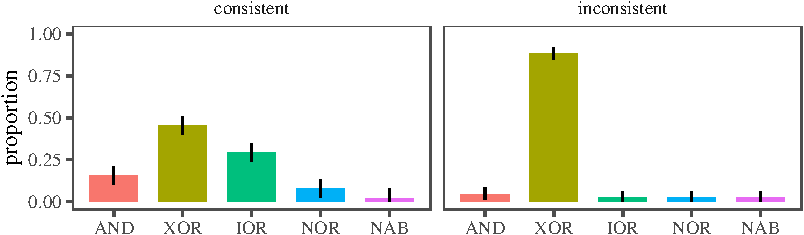
\includegraphics{figs/consistencyPlot-1} 

}

\caption{Connective interpretations in disjunctions with consistent and inconsistent disjuncts.}\label{fig:consistencyPlot}
\end{figure}

Figure \ref{fig:consistencyPlot} shows the proportions of connective interpretations in disjunctions with consistent vs.~inconsistent disjuncts. When the disjuncts were consistent, the interpretation could be exclusive (XOR), inclusive (IOR), or conjunctive (AND). When the disjuncts were inconsistent, a disjunction almost always received an exclusive interpretation. These results suggest that the exclusive interpretation of a disjunction often stems from the inconsistent or contradictory nature of the disjuncts themselves.{[}\^{}It should be noted here that in all \emph{and}-examples, the disjuncts were consistent. This is not surprising given that inconsistent meanings with \emph{and} result in a contradiction. The only exception to this was one example where the mother was mentioning two words as antonyms: \enquote{short and tall}. This example is quite different from the normal utterances given that it is meta-linguistic and list words rather than asserting the content of the words.{]} In Figure \ref{fig:consistencyByintonationPlot}, we break down interpretations by both intonation and consistency. The results show a clear pattern: disjunctions are interpreted as exclusive XOR when they carry either inconsistent disjuncts or a rise-fall intonation. If the disjunction has consistent disjuncts and carries a rising intonation, it is most likely interpreted as inclusive IOR. This pattern suggests that using disjunct consistency and sentence intonation, a learner can reliably separate the exclusive and inclusive interpretations of disjunction.

\begin{figure}[tb]

{\centering 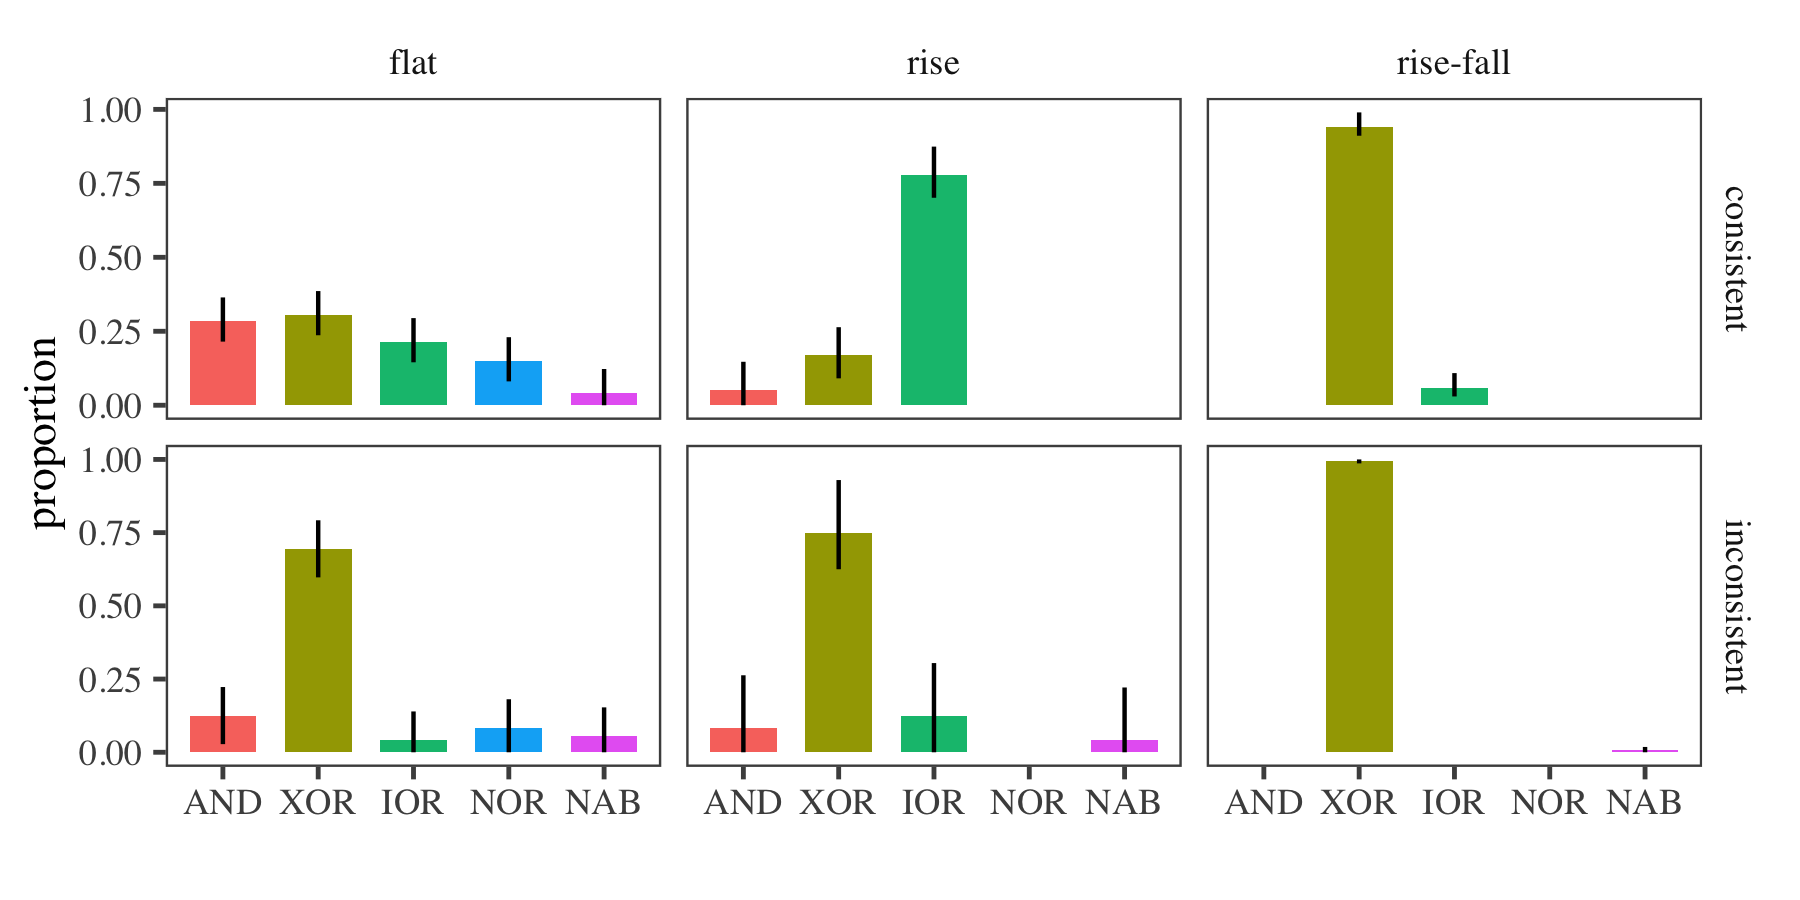
\includegraphics{figs/consistencyByintonationPlot-1} 

}

\caption{Interpretations of and/or in the three intonation contours flat, rising, and rise-fall.}\label{fig:consistencyByintonationPlot}
\end{figure}

\begin{figure}[tb]

{\centering 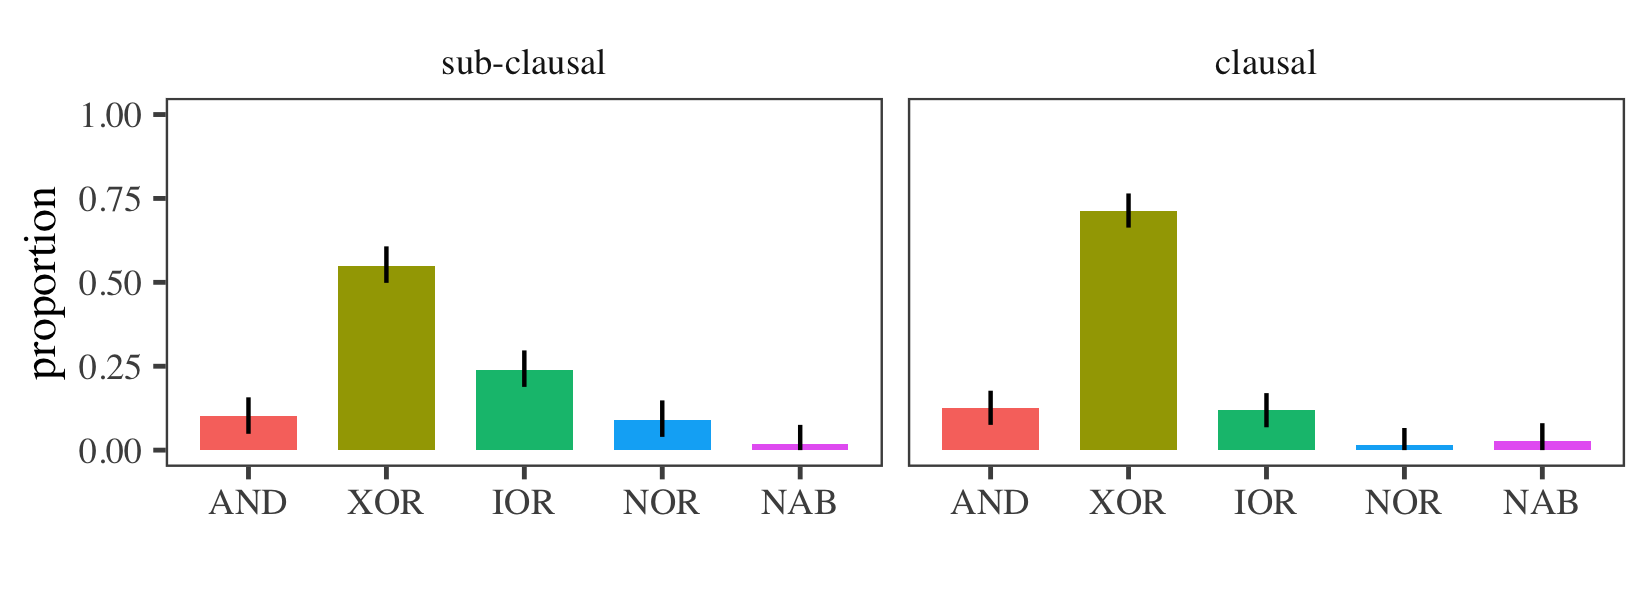
\includegraphics{figs/syntaxPlot-1} 

}

\caption{Connective interpretations in clausal and sub-clausal disjunctions.}\label{fig:syntaxPlot}
\end{figure}

Figure \ref{fig:syntaxPlot} shows connective interpretations by the syntactic level of the disjunction. The results suggest a small effect of clausal level disjuncts. Disjunctions were more likely to be interpreted as exclusive when their disjuncts were clauses or verbs rather than nominals, adjectives, or prepositions (all sub-clausal units).

\begin{figure}[tb]

{\centering 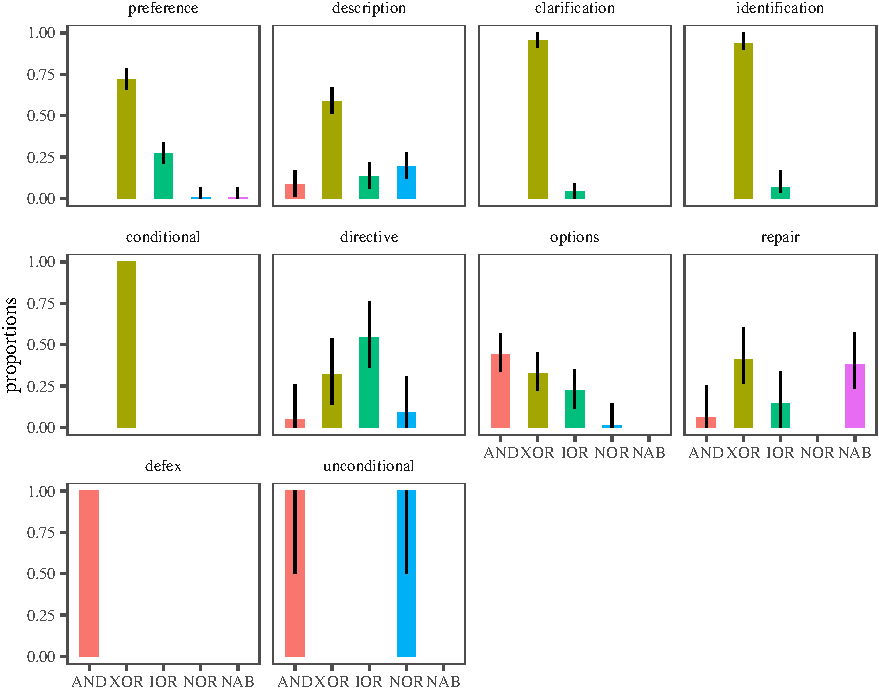
\includegraphics{figs/speechActPlot-1} 

}

\caption{Connective interpretations in different communicative functions.}\label{fig:speechActPlot}
\end{figure}

Finally, figure \ref{fig:speechActPlot} shows the proportions of connective interpretations in the 10 different communicative functions we defined. The results show that certain functions increase the likelihood of some connective interpretations. An exclusive (XOR) interpretation of \emph{or} is common in acts of clarification, identification, stating/asking preferences, stating/asking about a description, or making a conditional statements. These results are consistent with expectations on the communicative intentions of that these utterances carry. In clarifications, the speaker needs to know which of two alternatives the other party meant. Similarly in identifications, speaker needs to know which category does a referent belongs to. In preferences, parents seek to know which of two alternatives the child wants. Even though descriptions could be either inclusive or exclusive, in the current sample, most descriptions were questions about the state of affairs and required the child to provide one of the alternatives as the answer. In conditionals such as \enquote{come here or you are grounded}, the point of the threat is that only one disjunct can be true: either \enquote{you come and you are not grounded} or \enquote{you don't come and you are grounded}.

Repairs often received an exclusive (XOR) or a second-disjunct-true (NAB) interpretation. This is expected given that in repairs the speaker intends to say that the first disjunct is incorrect or inaccurate. Unconditionals and definitions/examples always had a conjunctive (AND) interpretation. Again, this is to be expected. In such cases the speaker intends to communicate that all options apply. If the mother says that \enquote{cats are animals like lions or tigers}, she intends to say that both lions and tigers are cats, and not one or the other. Interestingly, in some cases (not all), \emph{or} is replaceable by \emph{and}: \enquote{cats are animals like lions and tigers}. In unconditionals, the speaker communicates that in both alternatives, a certain proposition holds. For example, if the mother says \enquote{ready or not, here I come!}, she communicates that \enquote{I come} is true in both cases where \enquote{you are ready} and \enquote{you are not ready}.

Options were often interpreted either as conjunctive (AND) or inclusive (IOR). The category \enquote{options} contained examples of free-choice inferences such as \enquote{you could drink orange juice or apple juice}. This study found free-choice examples much more common than the current literature on the acquisition of disjunction suggests. Finally, directives received either an IOR or XOR interpretation. It is important to note here that the most common communicative function in the data were preferences and descriptions. Other communicative functions such as unconditionals or options were fairly rare. Despite their infrequent appearance, these constructions must be learned by children at some point, since almost all adults know how to interpret them. It is clear from the investigation here that any learning account for function word meaning/interpretation also needs to account for how such infrequent constructions are learned.

\hypertarget{discussion}{%
\subsubsection{Discussion}\label{discussion}}

The goal of this study was to discover the cues in child-directed speech that could help children learn the interpretations of a disjunction. The study presented 1000 examples of \emph{and} and \emph{or} in child-directed speech, annotated for their truth-conditional interpretation, as well as five candidate cues to their interpretation: (1) Utterance Type; (2) Intonation Type; (3) Syntactic Level; (4) Conceptual Consistency; (5) Communicative Function. Like Morris (2008), this study found that the most common interpretations of \emph{and} and \emph{or} are conjunction AND and exclusive disjunction XOR respectively. However, we found many inclusive and conjunctive instances of \emph{or} as well.

The most likely interpretation of a disjunction depended on the cues that accompanied it. A disjunction was most likely exclusive if the alternatives were inconsistent (i.e.~contradictory). A disjunction was either inclusive or exclusive if it appeared in a question. Within questions, a disjunction was most likely exclusive if the intonation was rise-fall. If the intonation was rising, the question was interpreted as inclusive. The syntactic category of the disjuncts could also provide information for interpretation. If the disjuncts were clausal then it was more likely for the disjunction to be interpreted as exclusive, even though this effect was small. Finally, specific communicative functions required specific interpretations of the connective. \emph{Or} often received a conjunctive interpretation in the following contexts: defining terms and providing examples, enumerating options, and in unconditional constructions. These results suggest that a learner can rely on cues that accompany a disjunciton for its interpretation. In the next section, we develop a computational model to test this hypothesis more formally.

\hypertarget{study-4-learning-to-interpret-a-disjunction}{%
\section{Study 4: Learning to interpret a disjunction}\label{study-4-learning-to-interpret-a-disjunction}}

Given the wide range of interpretations that \emph{or} can have, how can children learn to interpret it correctly? This is what study @ref addresses. In doing so, it also provides a solution to the puzzle of learning disjunction. To remind you about the puzzle, previous research have shown that the majority of \emph{or}-examples children hear are exclusive. However, comprehension studies report that between the ages of three and five, children can interpret \emph{or} as inclusive disjunction in declarative sentences (Crain, 2012). The finding of the comprehension studies and the corpus studies taken together present a learning puzzle: how can children learn to interpret \emph{or} as inclusive if they mostly hear exclusive examples? This chapter provides a solution by developing a cue-based account for children's acquisition of connectives. More generally, the account proposed in this chapter is helpful for learning words with multiple interpretations when one interpretation dominates the learner's input.

\hypertarget{cues-to-coordinator-meanings}{%
\subsection{Cues to coordinator meanings}\label{cues-to-coordinator-meanings}}

Three important compositional cues can help learners in restricting their hypotheses to coordinator meanings. First, as pointed out by Haspelmath (2007), coordination has specific compositional properties. Coordinators combine two or more units of the same type and return a larger unit of the same type. The larger unit has the same semantic relation with the surrounding words as the smaller units would have had without coordination. These properties separate coordinators from other function words such as articles, quantifiers, numerals, prepositions, and auxiliaries which are not used to connect sentences or any two similar units for that matter. In fact, the special syntactic properties of coordinators have compelled syntactic theories to consider specific rules for coordination.

The literature on syntactic bootstrapping suggests that children can use syntactic properties of the input to limit their word meaning hypotheses to the relevant domain (Brown, 1957; Gleitman, 1990; see Fisher, Gertner, Scott, \& Yuan, 2010 for a review). In the current 1073 annotations of conjunction and disjunction, I found that \emph{and} and \emph{or} connected sentences/clauses 56\% of the time. This pattern is unexpected for any other class of function words and it is possible that the syntactic distribution of coordinators cue the learners to the space of sentential connective meanings.

Second, in the annotation study we found that \emph{and} never occurs with inconsistent coordinands (e.g. \enquote{clean and dirty}) while \emph{or} commonly does (e.g. \enquote{clean or dirty}). The inconsistency of the coordinands can cue the learner to not consider conjunction as a meaning for the coordinator given that a conjunctive meaning would too often lead to a contradiction at the utterance level. On the other hand, choosing disjunction as the meaning avoids this problem. Third, the large scale study of Chapter \ref{corpus} found that \emph{or} is more likely to occur in questions than statements while \emph{and} is more likely in statements. Since questions often contain more uncertainty while statements are more informative, it is possible that these environments bias the learner towards selecting hypotheses that match this general communicative function. Disjunction is less informative than conjunction and it is possible that the frequent appearance of \emph{or} in questions cues learners to both its meaning as a disjunction as well as the ignorance inference commonly associated with it.

Finally, it is reasonable to assume that not all binary connective meanings shown in Figure \ref{fig:binaryLogicalConnectivess} are as likely for mapping. For example, coordinators that communicate tautologies or contradictions seem to be not good candidates for informative communication. Similarly, if A coordinated with B simply asserts the truth of A and says nothing about B, it is unclear why it would be needed if the language already has the means of simply asserting A. It is possible that pragmatic principles already bias the hypothesis space to favor candidates that are communicatively more efficient.

\begin{figure}[tb]

{\centering 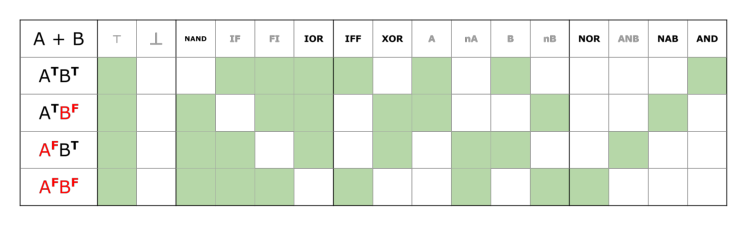
\includegraphics{figs/binaryLogicalConnectivess-1} 

}

\caption{The truth table for the 16 binary logical connectives. The rows represent the set of situations where zero, one, or both propositions are true. The columns represent the 16 possible connectives and their truth conditions. Green cells represent true situations.}\label{fig:binaryLogicalConnectivess}
\end{figure}

Even though these findings are suggestive, they need to be backed up by further observational and experimental evidence to show that children do actually use these cues in learning connective meanings. In the next section, I turn to the more specific issue of learning the correct interpretation of \emph{and} and \emph{or} from the input data. As in the case of number words, previous research has provided insight into how children comprehend a disjunction and what they hear from their parents. The main question is how children learn what they comprehend from what they hear. I turn to this issue in the next section.

\hypertarget{myaccount}{%
\subsection{\texorpdfstring{Learning to interpret \emph{and} and \emph{or}: A cue-based account}{Learning to interpret and and or: A cue-based account}}\label{myaccount}}

Previous comprehension studies have shown that children as early as age three can interpret a disjunction as inclusive (see Crain, 2012 for an overview). However, Morris (2008) showed that exclusive interpretations are much more common than other interpretations of disjunction in children's input. In Figure \ref{fig:interpretation}, I show the results of Chapter \ref{corpus}\enquote{s annotation study by grouping the disjunction interpretations into exclusive (EX) and inclusive (IN), i.e.~non-exclusive categories. These results replicate Morris} (2008) finding and reinforce a puzzle raised by Crain (2012): How can children learn the inclusive interpretation of disjunction when the majority of the examples they hear are exclusive? To answer this question, I draw on insights from the Gricean approach to semantics and pragmatics discussed in Chapter \ref{sempragLit}.

\begin{figure}[tb]

{\centering 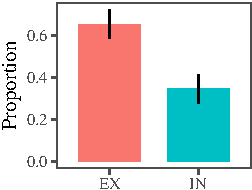
\includegraphics{figs/interpretation-1} 

}

\caption{Proportion of exclusive and inclusive interpretations of disjunction in child-directed speech. Error bars represent bootstrapped 95\% confidence intervals.}\label{fig:interpretation}
\end{figure}

Research in Gricean semantics and pragmatics has shown that the word \emph{or} is not the only factor relevant to the interpretation of a disjunction. It is not only the presence of the word \emph{or} that leads us to interpret a disjunction as inclusive, exclusive, or conjunctive, but rather the presence of \emph{or} along with several other factors such as intonation (Pruitt \& Roelofsen, 2013), the meaning of the disjuncts (Geurts, 2006), and the conversational principles governing communication (Grice, 1989). The interpretation and acquisition of the word \emph{or} cannot, therefore, be separated from all the factors that accompany it and shape its final interpretation.

In the literature on word learning and semantic acquisition, form-meaning mapping is often construed as mapping an isolated form such as \emph{gavagai} to an isolated concept such as \enquote{rabbit}. While this approach may be feasible for content words, it will not work for function words such as \emph{or}. First, the word \emph{or} cannot be mapped in isolation from its formal context. As Pruitt and Roelofsen (2013) showed, the intonation that accompanies a disjunction affects its interpretation. Therefore, a learner needs to pay attention to the word \emph{or} as well as the intonation contour that accompanies it. Second, the word \emph{or} cannot be mapped to its meaning isolated from the semantics of the disjuncts that accompany it. As Geurts (2006) argued, the exclusive interpretation is often enforced simply because the options are incompatible. For example, \enquote{to be or not to be} is exclusive simply because one cannot both be and not be. In addition, conversational factors play an important role in the interpretation of \emph{or} as Grice (1989) argued. In sum, the interpretation and acquisition of function words such as \emph{or} require the learner to consider the linguistic and nonlinguistic context of the word and map the meanings accordingly.

Previous accounts have adopted a model in which a function word such as \emph{or} is mapped directly to its most likely interpretation:

\emph{or} \(\rightarrow \oplus\)

This model is often used in cross-situational accounts of content words. Here I argue that the direct mapping of \emph{or} to its interpretation without consideration of its linguistic context is the primary cause of the learning puzzle for \emph{or}. Instead, I propose that the word \emph{or} is mapped to an interpretation in a context-dependent manner, along with the interpretive cues that accompany it such as intonation and disjunct semantics:

{[}connective: \emph{or}, Intonation: rise-fall, Disjuncts: inconsistent{]} \(\rightarrow \oplus\)

{[}connective: \emph{or}, Intonation: rising, Disjuncts: consistent{]} \(\rightarrow \lor\)

Figure \ref{fig:interpretationByIntonationAndConsistency} shows that the rate of exclusive interpretations change systematically when the data are broken down by intonation and consistency. Given a rise-fall intonation contour, a disjunction is almost always interpreted as exclusive. Similarly, if the propositions are inconsistent, the disjunction is most likely interpreted as exclusive. When either of these two features are absent, a disjunction is more likely to receive an inclusive interpretation.

\begin{figure}[tb]

{\centering 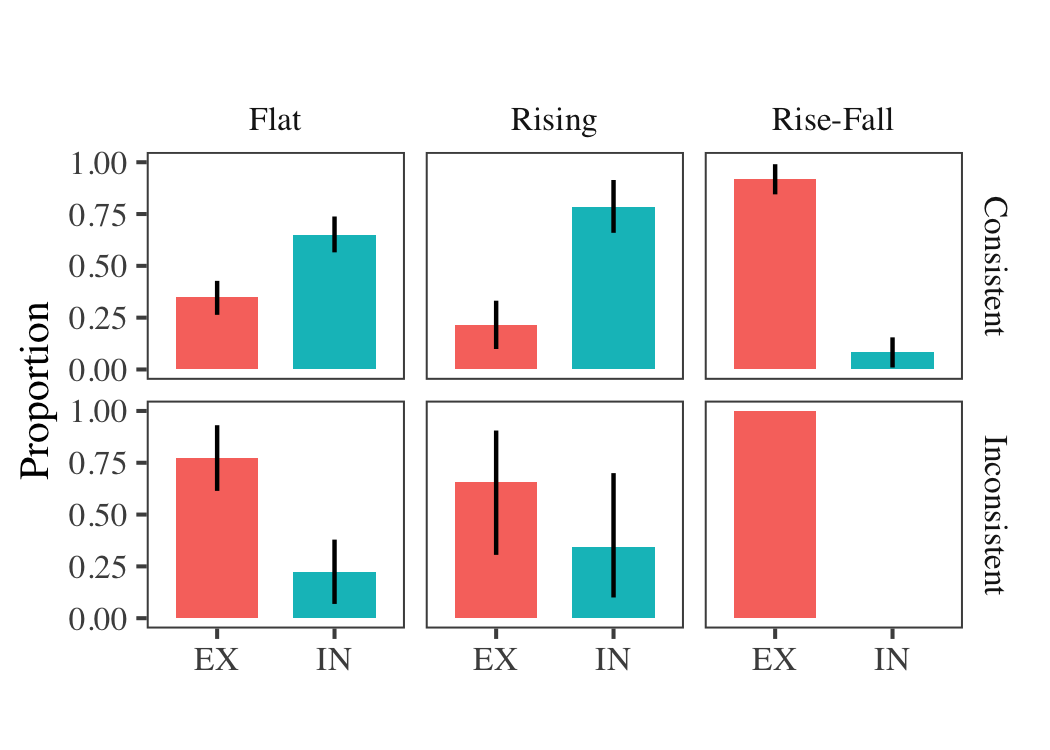
\includegraphics{figs/interpretationByIntonationAndConsistency-1} 

}

\caption{Exclusive and inclusive interpretations broken down by intonation (flat, rise, rise-fall) and consistency. Error bars represent bootstrapped 95\% confidence intervals.}\label{fig:interpretationByIntonationAndConsistency}
\end{figure}

In this account, it is not a single word that gets mapped to an interpretation but rather a cluster of features. This method has two advantages. First, it deals with the context dependency of disjunction interpretation. The learner knows that \emph{or} with some intonation has to be interpreted differently from one with another. Second, it allows the learner to pull apart the contribution of \emph{or} from the interpretive cues that often accompany it. In fact, analysis of all mapping clusters in which \emph{or} participates and generalization over them can help the learner extract the semantics of \emph{or} the way it is intended by Gricean accounts of semantics/pragmatics. For those skeptical of such an underlying semantics for \emph{or}, there is no need for further analysis of the mapping clusters. The meaning of \emph{or} as a single lexical item is distributed among the many mappings in which it participates. In the next section, I implement this idea using decision tree learning.

A decision tree is a classification model structured as a hierarchical tree with nodes, branches, and leaves (Breiman, 2017). The tree starts with an initial node, called the root, and branches into more nodes until it reaches the leaves. Each node represents the test on a feature, each branch represents an outcome of the test, and each leaf represents a classification label. Using a decision tree, observations can be classified or labeled based on a set of features.

Decision trees have several advantages for modeling cue-based accounts of semantic acquisition. First, decision trees use a set of features to predict the classification of observations. This is analogous to using cues to predict the correct interpretation of a word or an utterance. Second, unlike many other machine learning techniques, decision trees result in models that are interpretable. Third, the order of decisions or features used for classification is determined based on information gain. Features that appear higher (earlier) in the tree are more informative and helpful for classification. Therefore, decision trees can help us understand which cues are probably more helpful for the acquisition and interpretation of a word.

Decision tree learning is the construction of a decision tree from labeled training data. This section applies decision tree learning to the annotated data of Study 3 by constructing random forests (Breiman, 2001; Ho, 1995). In random forest classification, multiple decision trees are constructed on subsets of the data, and each tree predicts a classification. The ultimate outcome is a majority vote of each trees classification. Since decision trees tend to overfit data, random forests control for overfitting by building more trees and averaging their results. \textbf{(Citation)} Next section discusses the methods used in constrcting the random forests for interpreting connectives \emph{or}/\emph{and}.

\hypertarget{methods-2}{%
\subsubsection{Methods}\label{methods-2}}

The random forest models were constructed using python's Sci-kit Learn package (Pedregosa et al., 2011). The annotated data had a feature array and a connective interpretation label for each connective use. Connective interpretations included exclusive (XOR), inclusive (IOR), conjunctive (AND), negative inclusive (NOR), and NPQ which states that only the second proposition is true. The features or cues used included all other annotation categories: intonation, consistency, syntactic level, utterance type, and communicative function. All models were trained with stratified 10-Fold cross-validation to reduce overfitting. Stratified cross-validation maintains the distribution of the initial data in the random sampling to build cross validated models. Maintaining the data distribution ensures a more realistic learning environment for the forests. Tree success was measured with F1-Score, harmonic average of precision and recall \textbf{(Citation)}.

First a grid search was run on the hyperparamter space to establish the number of trees in each forest and the maximum tree depth allowable. The grid search creates a grid of all combinations of forest size and tree depth and then trains each forest from this grid on the data. The forests with the best F1-score and lowest size/depth are reported. **(Citation*)\textbf{ The default number of trees for the forests was set to 20, with a max depth of eight and a minimum impurity decrease of 0. Impurity was measured with gini impurity, which states the odds that a random member of the subset would be mislabled if it were randomly labeled according to the distribution of labels in the subset. }(Citation)**

Decision trees were fit with high and low minimum gini decrease values. High minimum gini decrease results in a tree that does not use any features for branching. Such a tree represents the baseline or traditional approach to mapping that directly maps a word to its most likely interpretation. Low minimum gini decrease allows for a less conservative tree that uses multiple cues/features to predict the interpretation of a disjunction. Such a tree represents the cue-based context-sensitive account of word learning discussed in the previous section.

\hypertarget{results-1}{%
\subsubsection{Results}\label{results-1}}

We first present the results of the random forests in the binary classification task. The models were trained to classify exclusive and inclusive interpretations of disjunction. For visualization of trees, we selected the highest performing tree in the forest by testing each tree and selecting for highest F1 score. While the forests performance is not identical to the highest performing tree, the best tree gives an illustrative example of how the tree performs.

Figure \ref{fig:binaryBaseline} shows the best performing decision tree with high minimum gini decrease. As expected, a learner that does not use any cues would interpret \emph{or} as exclusive all the time. This is the baseline model. Figure \ref{fig:binaryCueBased} shows the best performing decision tree with low minimum gini decrease. The tree has learned to use intonation and consistency to classify disjunctions as exclusive or inclusive. As expected, if the intonation is rise-fall or the disjuncts are inconsistent, the interpretation is exclusive. Otherwise, the disjunction is classified as inclusive.

\begin{figure}
\centering
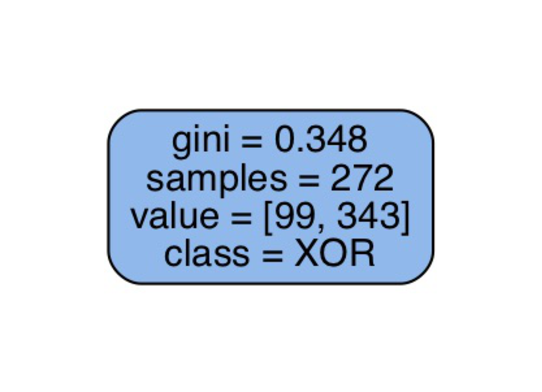
\includegraphics{figs/binaryBaseline-1.pdf}
\caption{\label{fig:binaryBaseline}Baseline tree grown with minimum impurity decrease of 0.2. The tree always classifies examples of disjunction as exclusive.}
\end{figure}

\begin{figure}
\centering
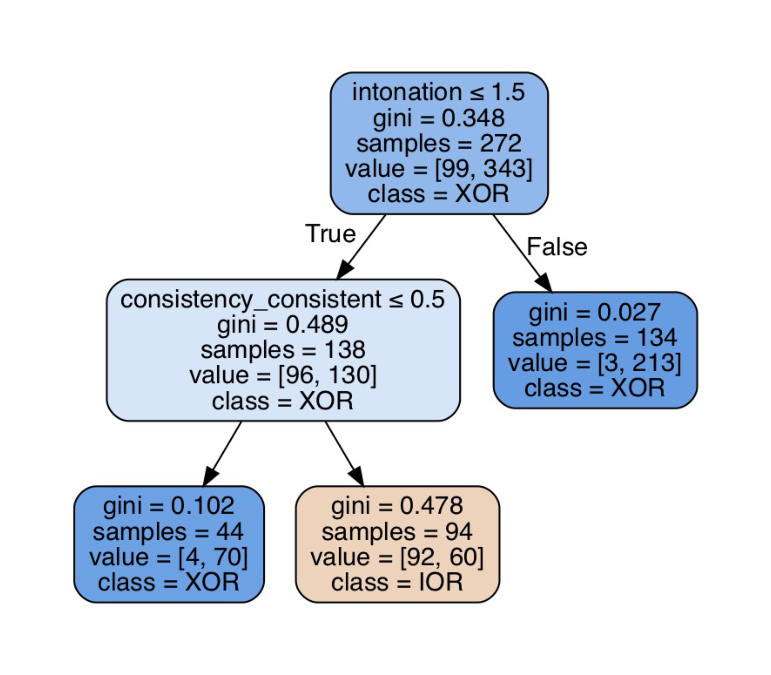
\includegraphics{figs/binaryCueBased-1.pdf}
\caption{\label{fig:binaryCueBased}Cue-based tree grown with minimum impurity decrease of 0.01. The tree classifies examples of disjunction with rise-fall intonation as exclusive (intonation \textgreater{} 1.5). If the intonation is not rise-fall but the disjuncts are inconsistent (consistency \textless{} 0.5), then the disjunction is still classified as exclusive. However, if neither of these two hold, the disjunction is classified as inclusive.}
\end{figure}

Figure \ref{fig:XorBinary} shows the average F1 scores of the baseline and cue-based models in classifying exclusive examples. The models perform relatively well and similar to each other, but the cue-based model performs slightly better. The real difference between the baseline model and the cue-based model is in their performance on inclusive examples. Figure \ref{fig:IorBinary} shows the F1 score of the forests as a function of the training size in classifying inclusive examples. As expected, the baseline model performs very poorly while the cue-based model does a relatively good job and improves with more examples.

\begin{figure}
\centering
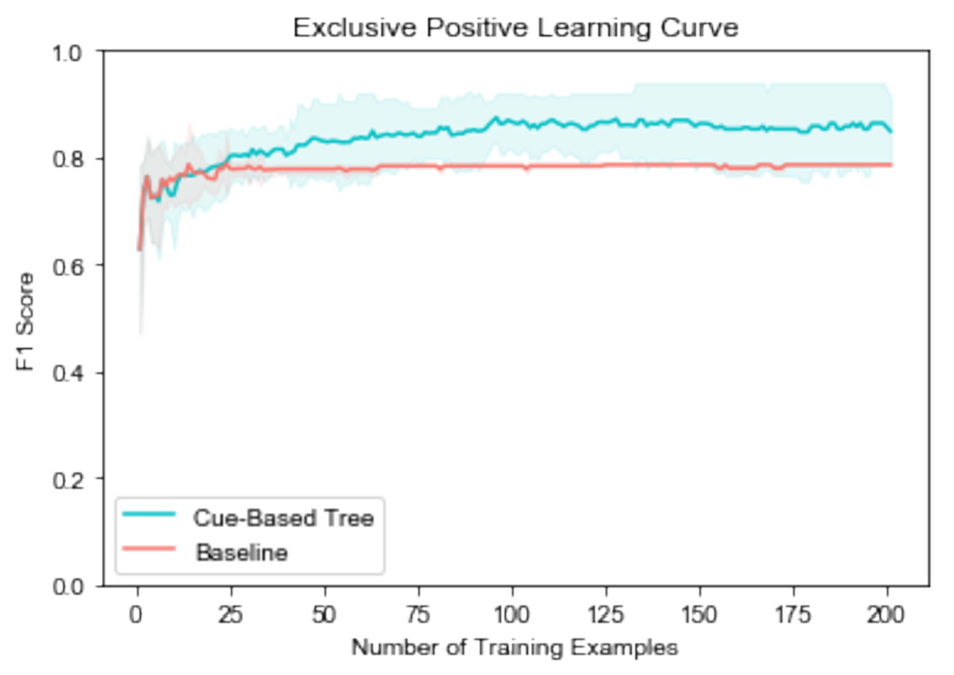
\includegraphics{figs/XorBinary-1.pdf}
\caption{\label{fig:XorBinary}The average F1 score for class XOR (exclusive) as a function of the number of training examples in the baseline and cue-based models. The colored shades show the 95\% confidence intervals.}
\end{figure}

\begin{figure}
\centering
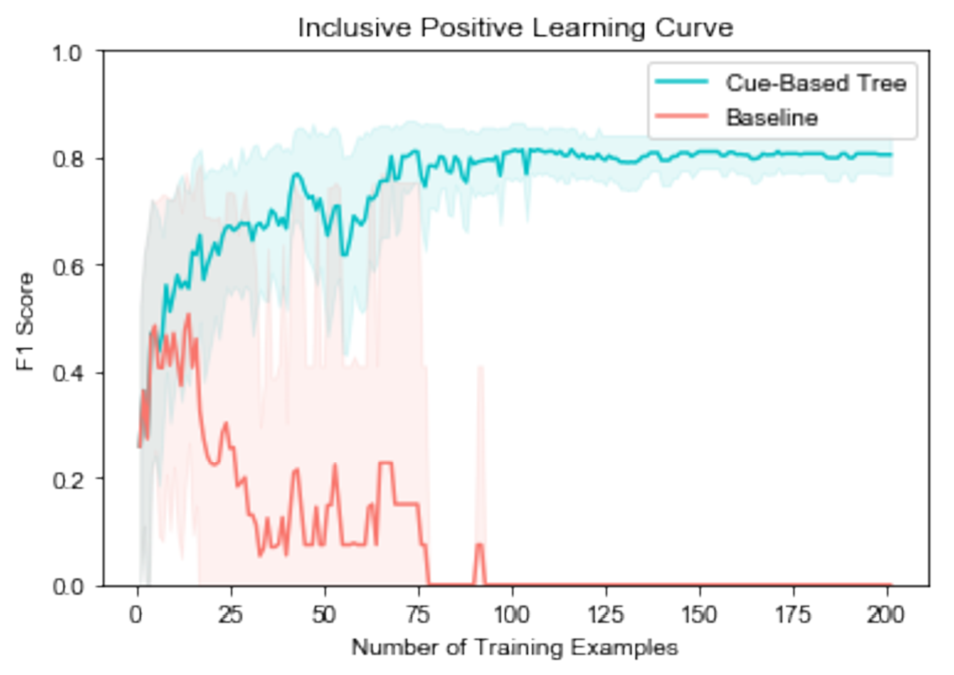
\includegraphics{figs/IorBinary-1.pdf}
\caption{\label{fig:IorBinary}The average F1 score for class IOR (inclusive) as a function of the number of training examples in the baseline and cue-based models. The colored shades show the 95\% confidence intervals.}
\end{figure}

Next, we use decision tree learning in a ternary classification task. The model uses features to interpret a coordination with \emph{and} and \emph{or} as inclusive (IOR), exclusive (XOR), or conjunctive (AND). Figure \ref{fig:ternaryBaseline} shows the baseline decision tree with high minimum gini decrease, which only uses the presence of the words \emph{or}/\emph{and} to interpret conjunction and disjunction. As expected, the tree interprets a coordination with \emph{and} as a conjunction and one with \emph{or} as exclusive disjunction. Figure \ref{fig:ternaryCueBased} shows the cue-based decision tree with low minimum gini decrease. In addition to the presence of \emph{and} and \emph{or}, the tree uses intonation, consistency, communicative function, and utterance type to distinguish exclusive, inclusive, and conjunctive uses of disjunction. In short, a disjunction that is rise-fall, inconsistent, or has a conditional communicative function is classified as exclusive. Otherwise the disjunction is classified as inclusive. The tree also finds conjunctive interpretations of disjunction more likely in declarative sentences than interrogatives.

\begin{figure}
\centering
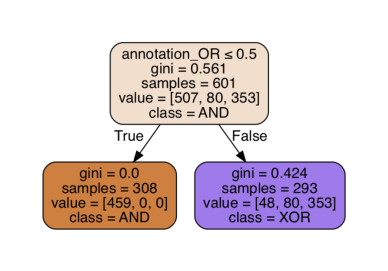
\includegraphics{figs/ternaryBaseline-1.pdf}
\caption{\label{fig:ternaryBaseline}The baseline tree grown on conjunctions and disjunctions with minimum impurity decrease of 0.2. The tree uses the words \textit{and/or} and classifies them as conjunction and exclusive disjunction respectively.}
\end{figure}

\begin{figure}
\centering
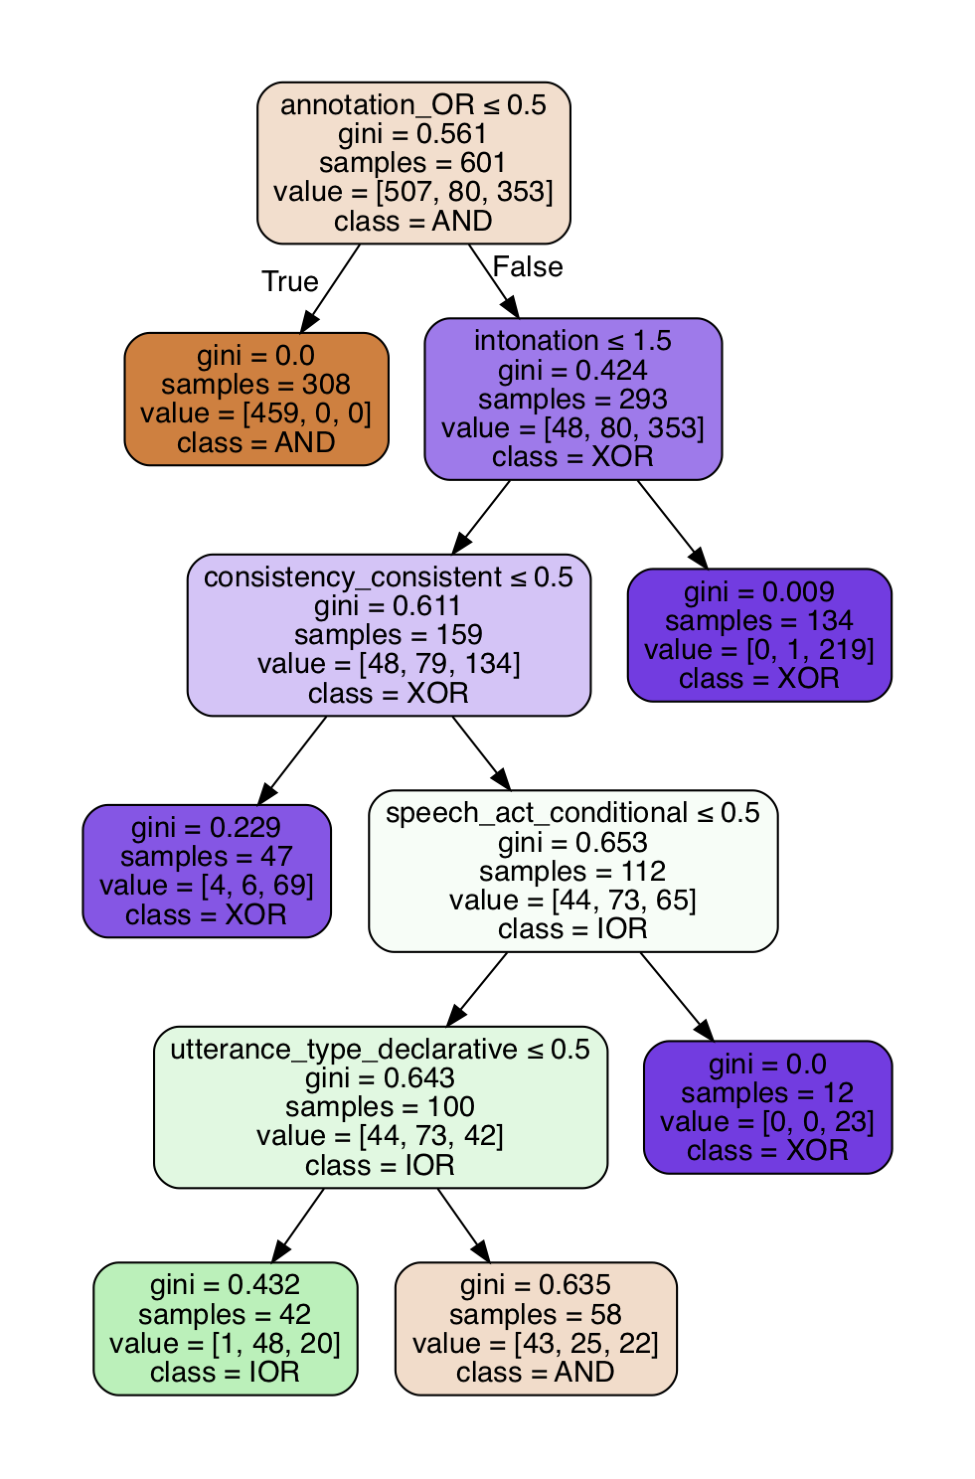
\includegraphics{figs/ternaryCueBased-1.pdf}
\caption{\label{fig:ternaryCueBased}The cue-based tree grown on conjunctions and disjunctions with minimum impurity decrease of 0.01. After using the words \textit{and/or}, the tree uses intonation, consistency, and the conditional communicative function to classify a large number of exclusive cases. Then it uses utterance type (interrogative) to label inclusive cases.}
\end{figure}

Figure \ref{fig:ANDintermediate} shows the average F1 score of the conjunctive interpretations (AND) for the baseline and the cue-based models. Since the vast majority of the conjunctive interpretations are predicted by the presence of the word \emph{and}, the baseline and cue-based models show similar performances. Setting aside conjunction examples, Figure \ref{fig:ANDintermediateDis} shows the average F1 score of the AND interpretation of disjunction only. Here we see that the cue-based model performs better than the default model in guessing conjunctive interpretations of disjunction. The informal analysis of the trees suggest that the model does this by using the \enquote{speech act} cue. Figure \ref{fig:XORintermediate} shows the average F1-score of the exclusive interpretations (XOR) for the baseline and the cue-based models. The cue-based model does slightly better than the baseline model. As before, the most important improvement comes in identifying inclusive examples. Figure \ref{fig:IORintermediate} shows the average F1-score of the inclusive interpretations (IOR) for both baseline and cue-based models. The baseline model performs very poorly while the cue-based model is capable of classifying inclusive examples as well.

\begin{figure}
\centering
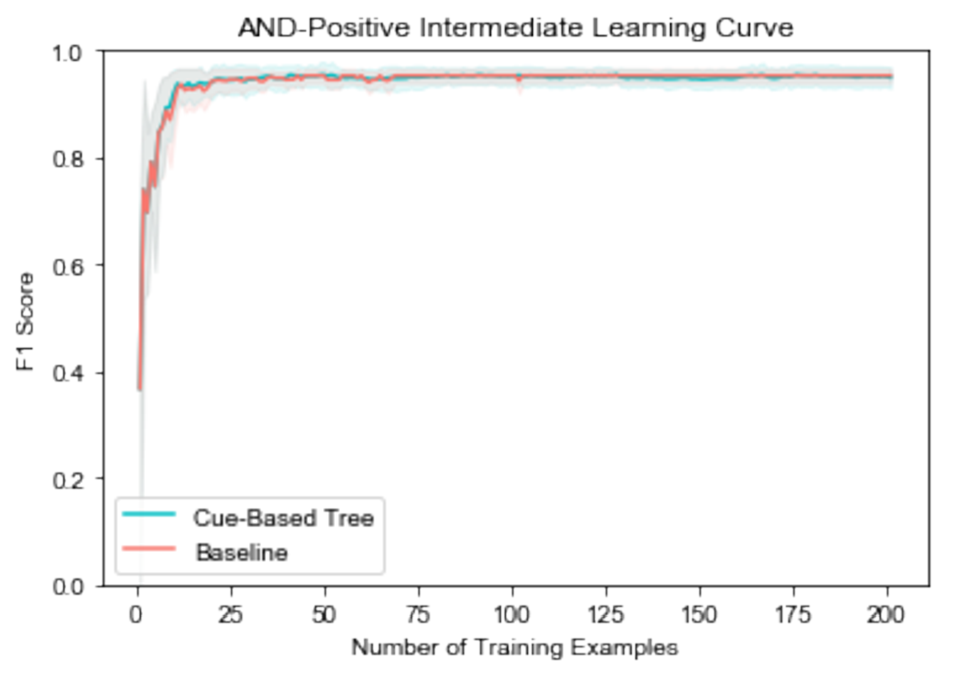
\includegraphics{figs/ANDintermediate-1.pdf}
\caption{\label{fig:ANDintermediate}The average F1 score for class AND as a function of the number of training examples in the baseline and cue-based models. The colored shades show the 95\% confidence intervals.}
\end{figure}

\begin{figure}
\centering
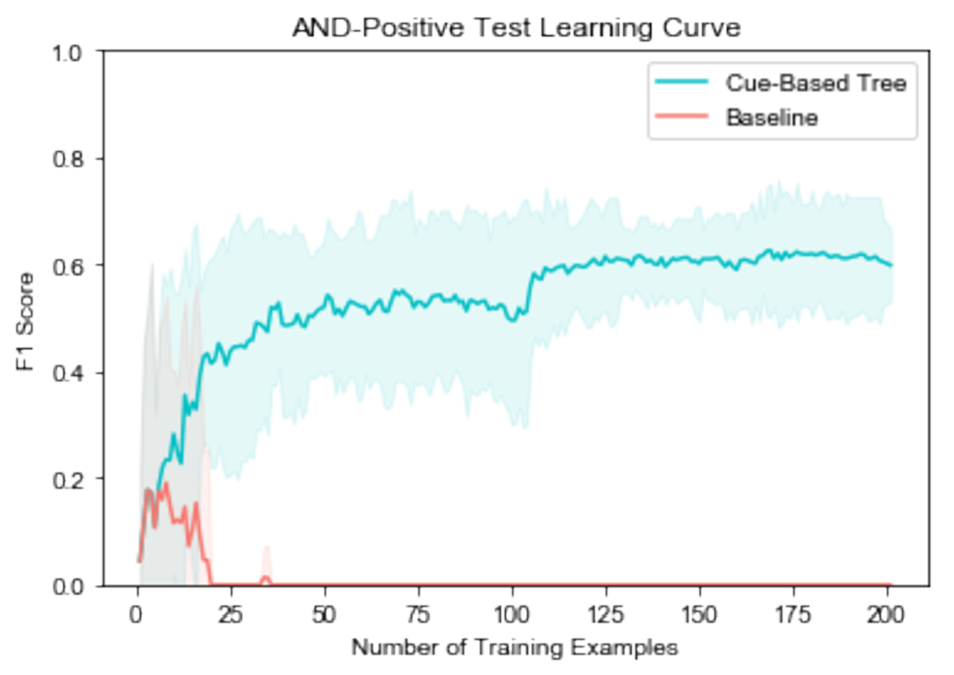
\includegraphics{figs/ANDintermediateDis-1.pdf}
\caption{\label{fig:ANDintermediateDis}The average F1 score for class AND of disjunction examles as a function of the number of training examples in the baseline and cue-based models. The colored shades show the 95\% confidence intervals.}
\end{figure}

\begin{figure}
\centering
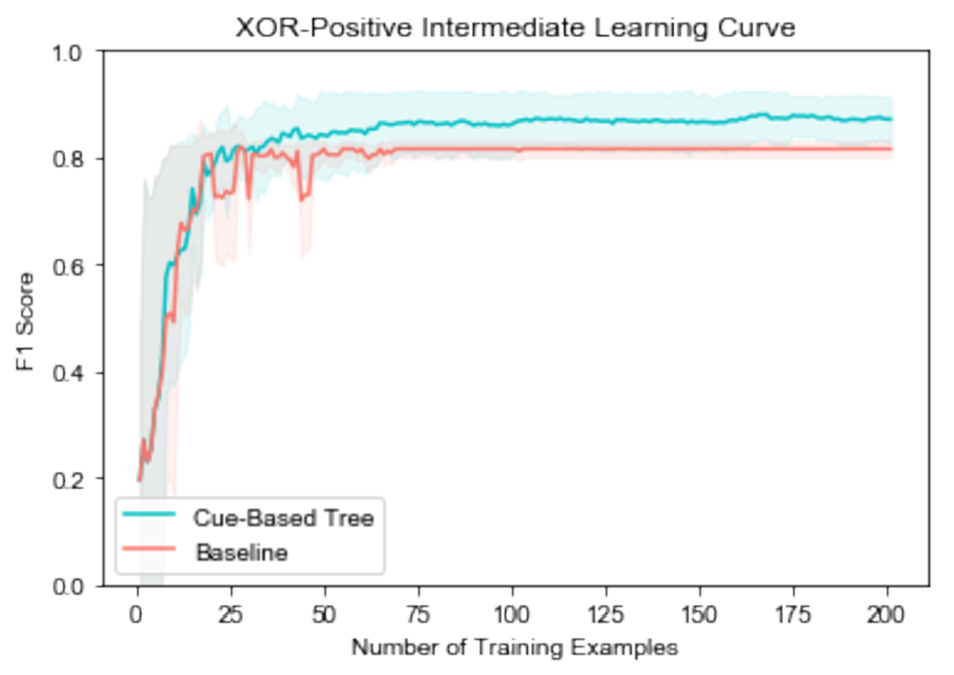
\includegraphics{figs/XORintermediate-1.pdf}
\caption{\label{fig:XORintermediate}The average F1 score for class XOR as a function of the number of training examples in the baseline and cue-based models. The colored shades show the 95\% confidence intervals.}
\end{figure}

\begin{figure}
\centering
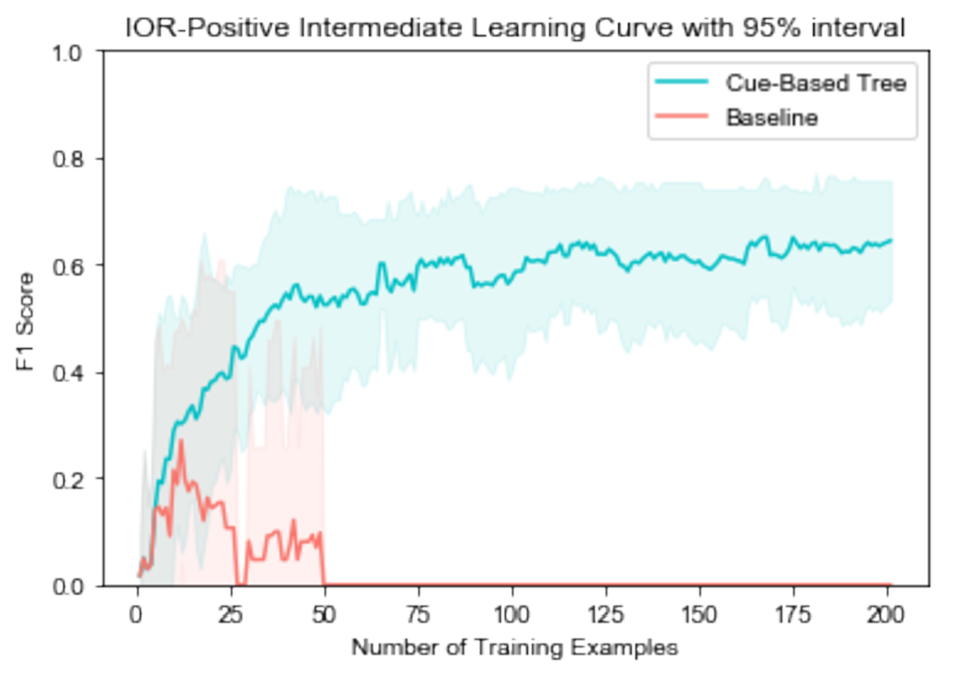
\includegraphics{figs/IORintermediate-1.pdf}
\caption{\label{fig:IORintermediate}The average F1 score for class IOR as a function of the number of training examples in the baseline and cue-based models. The colored shades show the 95\% confidence intervals.}
\end{figure}

Finally, welook at decision trees trained on the annotation data to predict all the interpretation classes for disjunction: AND, XOR, IOR, NOR, and NPQ. Figure \ref{fig:wholeBaseline} shows the baseline model that only uses the words \emph{and} and \emph{or} to classify. As expected, \emph{and} receives a conjunctive interpretation (AND) and \emph{or} receives an exclusive interpretation (XOR). Figure \ref{fig:wholeCueBased} shows the best example tree of the cue-based model. The leaves of the tree show that it recognizes exclusive, inclusive, conjunctive, and even negative inclusive (NOR) interpretations of disjunction. How does the tree achieve that? Like the baseline model, the tree first asks about the connective used: \emph{and} vs. \emph{or}. Then like the previous models, it asks about intonation and consistency. If the intonation is rise-fall, or the disjuncts are inconsistent, the interpretation is exclusive. Then it asks whether the sentence is an interrogative or a declarative. If interrogative, it guesses an inclusive interpretation. This basically covers questions with a rising intonation. Then the tree picks declarative examples that have conditional speech act (e.g. \enquote{give me the toy or you're grounded}) and labels them as exclusive. Finally, if negation is present in the sentence, the tree labels the disjunction as NOR.

\begin{figure}
\centering
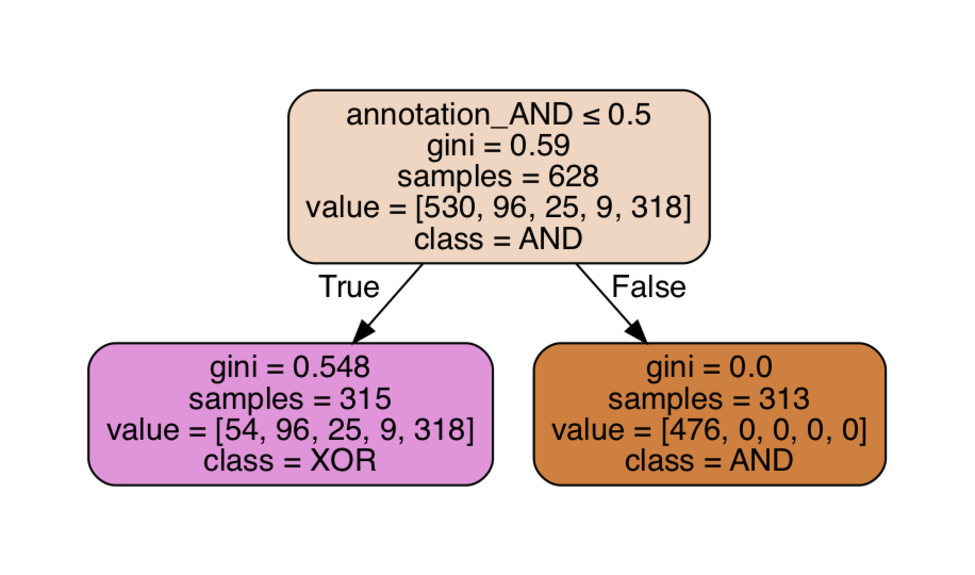
\includegraphics{figs/wholeBaseline-1.pdf}
\caption{\label{fig:wholeBaseline}The baseline tree grown on conjunctions and disjunctions with minimum impurity decrease of 0.2. The tree uses the words \textit{and/or} and classifies them as conjunction and exclusive disjunction.}
\end{figure}

\begin{figure}
\centering
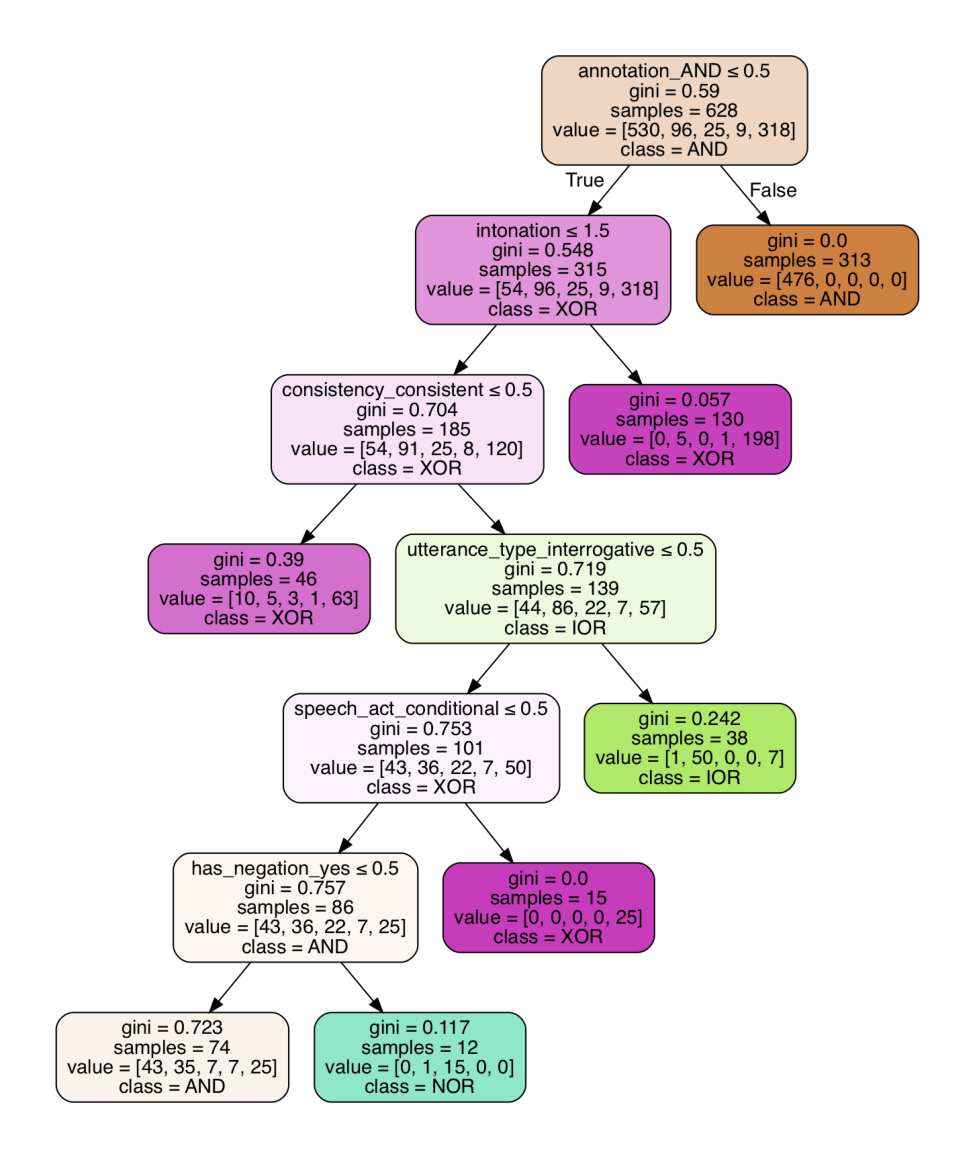
\includegraphics{figs/wholeCueBased-1.pdf}
\caption{\label{fig:wholeCueBased}The cue-based tree grown on conjunctions and disjunctions with minimum impurity decrease of 0.01. After using the words \textit{and/or}, the tree uses intonation and consistency to classify a large number of exclusive cases. Then it uses utterance type (interrogative) to label many inclusive cases, as well as the communicative function (conditional) to catch more exclusive examples. Finally, it asks whether the sentence has negation or not. If so, it classifies the negative inlusive examples as NOR.}
\end{figure}

Figures \ref{fig:ANDWhole}, \ref{fig:XORWhole}, and \ref{fig:IORWhole} show the average F1-scores for the conjunctive (AND), exclusive (XOR), and inclusive (IOR) interpretations as a function of training size. The results are similar to what wereported before with the ternary classification. While the cue-based model generally performs better than the baseline model, it shows substantial improvement in classifying inclusive cases.

\begin{figure}
\centering
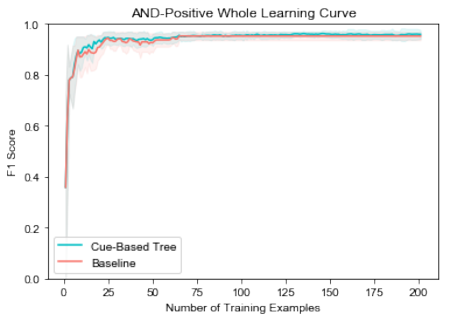
\includegraphics{figs/ANDWhole-1.pdf}
\caption{\label{fig:ANDWhole}The average F1 score for class AND as a function of the number of training examples in the baseline and cue-based models. The colored shades show the 95\% confidence intervals.}
\end{figure}

\begin{figure}
\centering
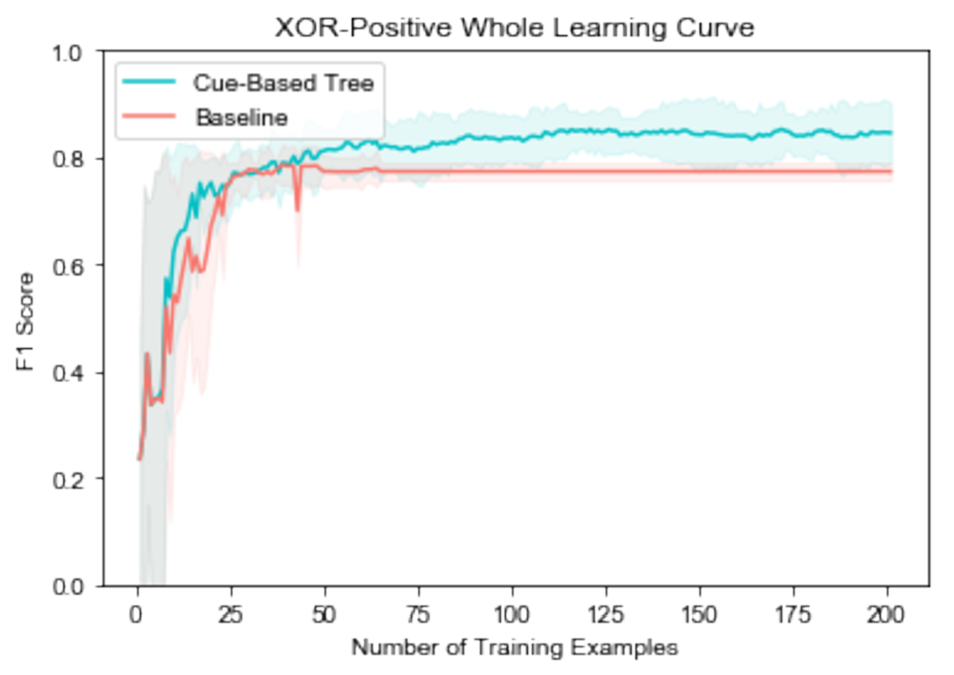
\includegraphics{figs/XORWhole-1.pdf}
\caption{\label{fig:XORWhole}The average F1 score for class XOR as a function of the number of training examples in the baseline and cue-based models. The colored shades show the 95\% confidence intervals.}
\end{figure}

\begin{figure}
\centering
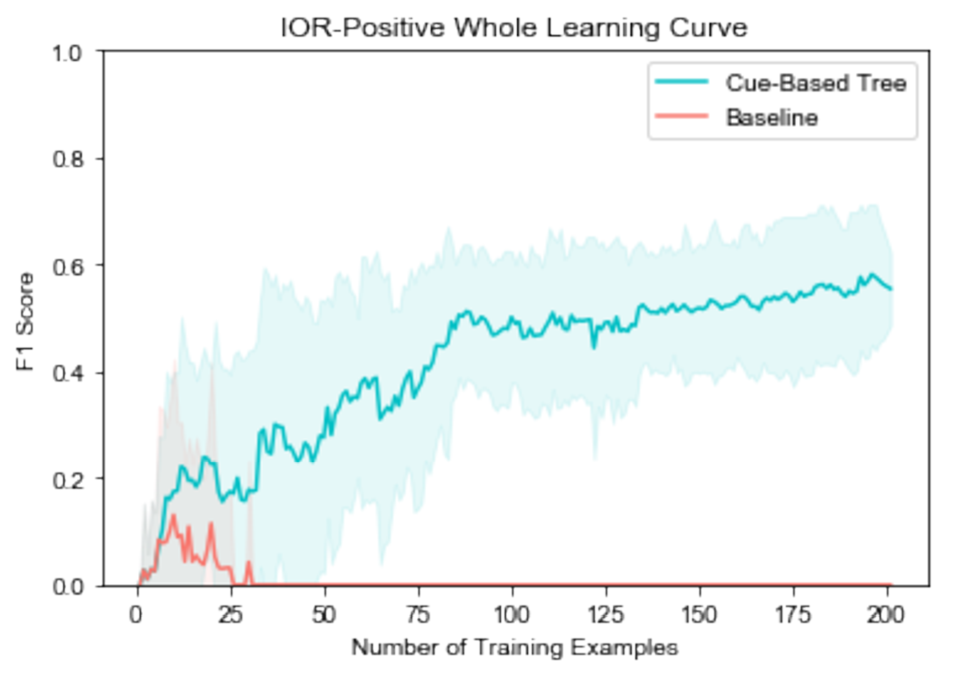
\includegraphics{figs/IORWhole-1.pdf}
\caption{\label{fig:IORWhole}The average F1 score for class IOR as a function of the number of training examples in the baseline and cue-based models. The colored shades show the 95\% confidence intervals.}
\end{figure}

Figure \ref{fig:NORWhole} shows the average F1-score for the negative inclusive interpretation as a function of training size. Compared to the baseline model, the cue-based model shows a substantially better performance in classifying negative sentences. The success of the model in classifying negative inclusive examples (NOR) suggests that the cue-based model offers a promising approach for capturing the scope relation of operators such as negation and disjunction. Here, the model learns that when negation and disjunction are present, the sentence receives a negative inclusive (NOR) interpretation. In other words, the model has learned the narrow-scope interpretation of negation and disjunction from the input data. In a language where negation and disjunction receive an XOR interpretation (not A or not B), the cue-based model can learn the wide-scope interpretation of disjunction.

\begin{figure}
\centering
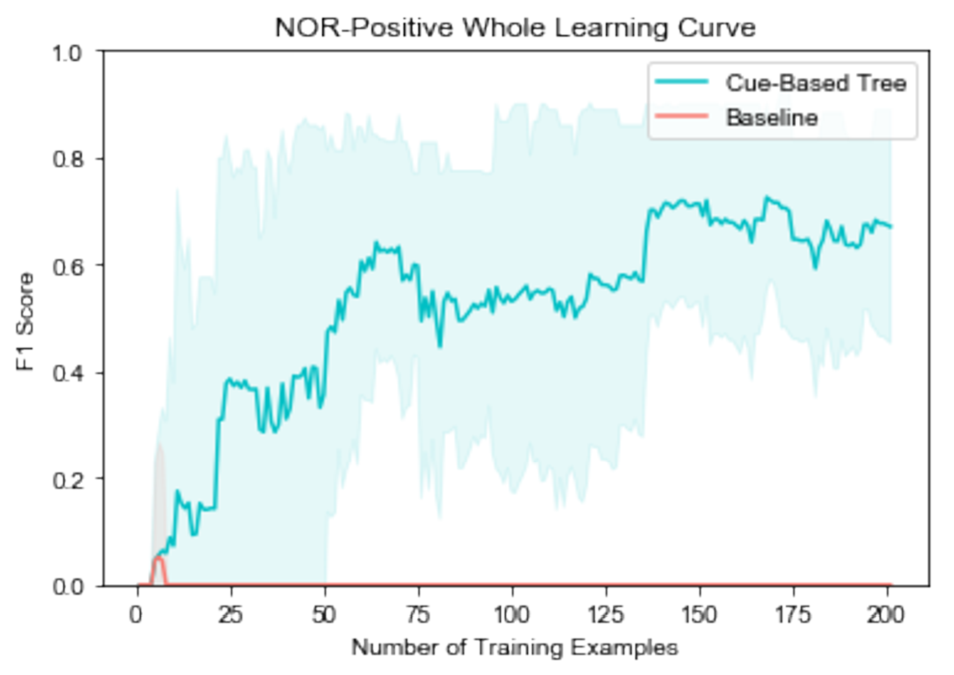
\includegraphics{figs/NORWhole-1.pdf}
\caption{\label{fig:NORWhole}The average F1 score for class NOR as a function of the number of training examples in the baseline and cue-based models. The colored shades show the 95\% confidence intervals.}
\end{figure}

Finally, Figure \ref{fig:NPQWhole} shows the average F1 score for the class NPQ. This interpretation suggested that the first disjunct is false but the second true. It was seen in examples of repair most often and the most likely cue to it was also the communicative function or speech act of repair. The results show that even though there were improvements in the cue-based model, they were not stable as shown by the large confidence intervals. It is possible that with larger training samples, the cue-based model can reliably classify the NPQ interpretations as well.

\begin{figure}
\centering
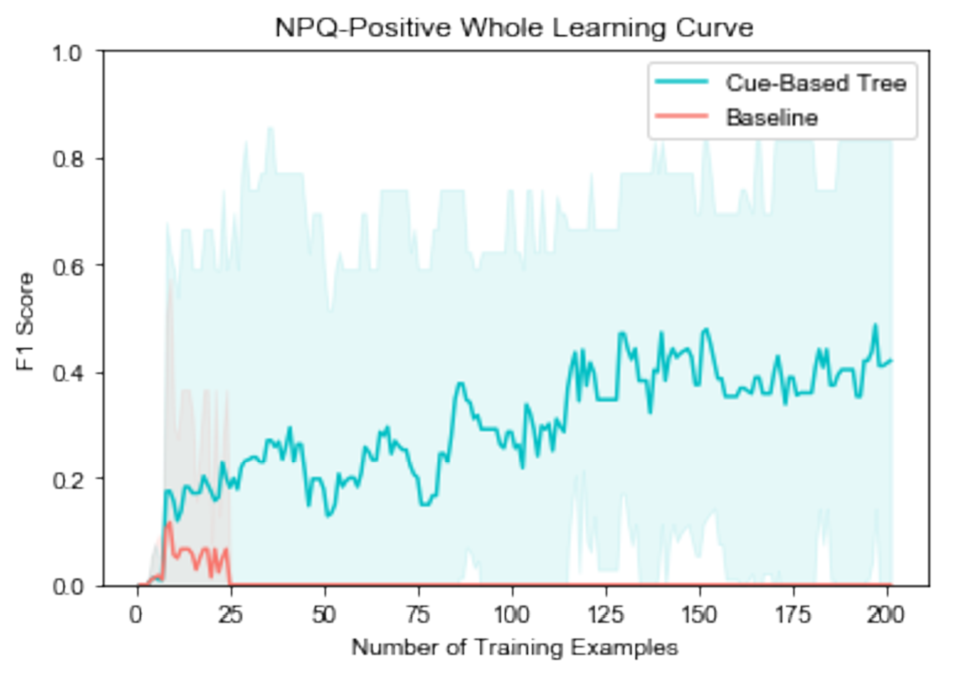
\includegraphics{figs/NPQWhole-1.pdf}
\caption{\label{fig:NPQWhole}The average F1 score for class NPQ as a function of the number of training examples in the baseline and cue-based models. The colored shades show the 95\% confidence intervals.}
\end{figure}

\hypertarget{discussion-1}{%
\subsection{Discussion}\label{discussion-1}}

We considered two accounts for the acquisition of function words. The first account was a baseline (context-independent) account that is used in vanilla cross-situational word learning: words are isolated and directly mapped to their most frequent meanings. The second account is what I called the cue-based context-dependent mapping in which words are mapped to meanings conditional on a set of present cues in the context. I argued that the puzzle of learning disjunction arises because in the baseline account, forms are mapped directly to meanings without considering the context of use. Under this account, the input statistics supports an exclusive interpretation for \emph{or}. However, comprehension studies show that children can interpret \emph{or} as inclusive. I showed that the cue-based account resolves this problem by allowing \emph{or} to be mapped to its interpretation according to the set of contextual cues that disambiguate it. The results of computational experiments with decision tree learning on data from child-directed speech suggested that such an approach can successfully learn to classify a disjunction is inclusive or exclusive. More broadly, cue-based context-dependent mapping is useful for the acquisition of ambiguous words and interpretations that are consistent but relatively infrequent in child-directed speech.

\hypertarget{conclusion}{%
\section{Conclusion}\label{conclusion}}

The case of disjunction shows that word learning requires to systmatically take different aspects of the linguistic and non-linguistic context into account. The meaning of a word such as \emph{or} cannot be learned independent of its context such as its intonation contour, the meaning of the coordinands it conjoins, or type of speech act it participates in.

\newpage

\hypertarget{references}{%
\section{References}\label{references}}

\hypertarget{appendix}{%
\section{Appendix}\label{appendix}}

\begin{figure}[tb]

{\centering 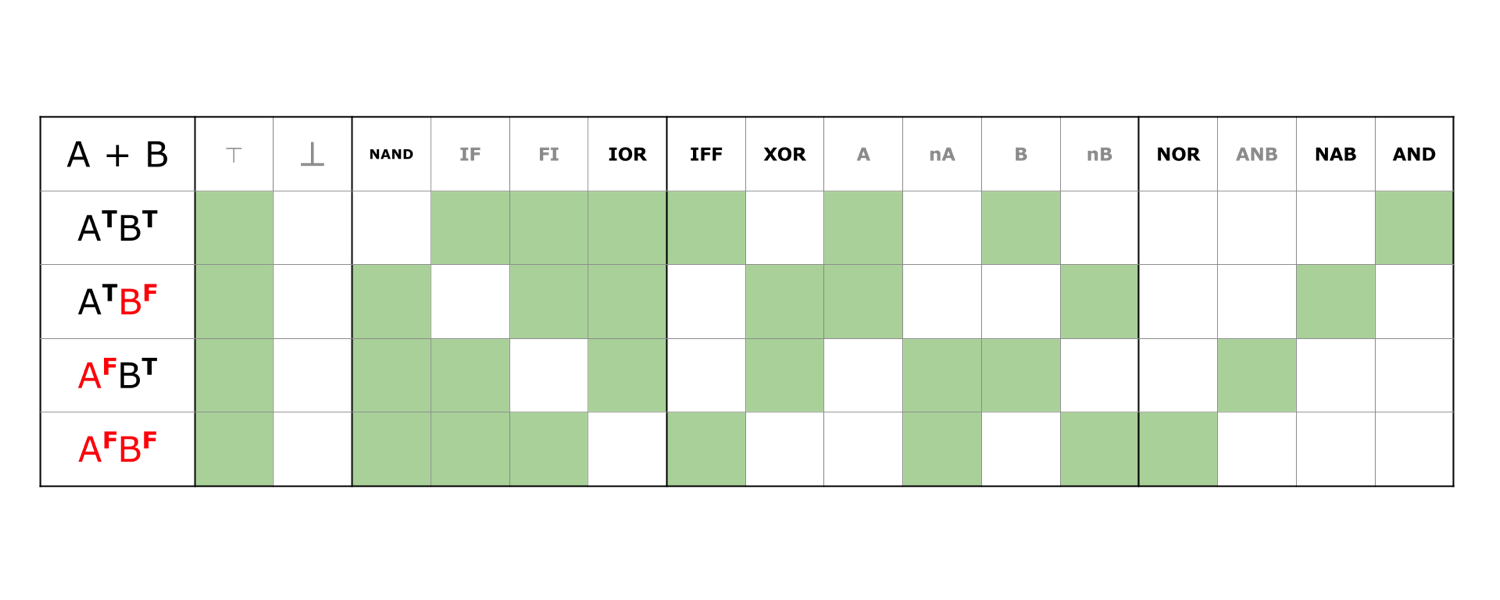
\includegraphics{figs/logicalConnectives-1} 

}

\caption{The truth table for the 16 binary logical connectives. The rows represent the set of situations where zero, one, or both propositions are true. The columns represent the 16 possible connectives and their truth conditions. Green cells represent true situations.}\label{fig:logicalConnectives}
\end{figure}

\hypertarget{annotation-categories-1}{%
\subsection{Annotation Categories}\label{annotation-categories-1}}

\begin{longtable}[]{@{}lll@{}}
\caption{\label{tab:connectiveInterpretaion} Annotation classes for connective interpretation}\tabularnewline
\toprule
\begin{minipage}[b]{0.06\columnwidth}\raggedright
Class\strut
\end{minipage} & \begin{minipage}[b]{0.36\columnwidth}\raggedright
Meaning\strut
\end{minipage} & \begin{minipage}[b]{0.49\columnwidth}\raggedright
Examples\strut
\end{minipage}\tabularnewline
\midrule
\endfirsthead
\toprule
\begin{minipage}[b]{0.06\columnwidth}\raggedright
Class\strut
\end{minipage} & \begin{minipage}[b]{0.36\columnwidth}\raggedright
Meaning\strut
\end{minipage} & \begin{minipage}[b]{0.49\columnwidth}\raggedright
Examples\strut
\end{minipage}\tabularnewline
\midrule
\endhead
\begin{minipage}[t]{0.06\columnwidth}\raggedright
AND\strut
\end{minipage} & \begin{minipage}[t]{0.36\columnwidth}\raggedright
Both propositions are true\strut
\end{minipage} & \begin{minipage}[t]{0.49\columnwidth}\raggedright
\emph{\enquote{I'm just gonna empty this and then I'll be out of the kitchen.} -- \enquote{I'll mix them together or I could mix it with carrot, too.}}\strut
\end{minipage}\tabularnewline
\begin{minipage}[t]{0.06\columnwidth}\raggedright
IOR\strut
\end{minipage} & \begin{minipage}[t]{0.36\columnwidth}\raggedright
One or both propositions are true\strut
\end{minipage} & \begin{minipage}[t]{0.49\columnwidth}\raggedright
\emph{\enquote{You should use a spoon or a fork.} -- \enquote{Ask a grownup for some juice or water or soy milk.}}\strut
\end{minipage}\tabularnewline
\begin{minipage}[t]{0.06\columnwidth}\raggedright
XOR\strut
\end{minipage} & \begin{minipage}[t]{0.36\columnwidth}\raggedright
Only one proposition is true\strut
\end{minipage} & \begin{minipage}[t]{0.49\columnwidth}\raggedright
\emph{\enquote{Is that a hyena? or a leopard?} -- \enquote{We're gonna do things one way or the other.}}\strut
\end{minipage}\tabularnewline
\begin{minipage}[t]{0.06\columnwidth}\raggedright
NOR\strut
\end{minipage} & \begin{minipage}[t]{0.36\columnwidth}\raggedright
Neither proposition is true\strut
\end{minipage} & \begin{minipage}[t]{0.49\columnwidth}\raggedright
\emph{\enquote{I wouldn't say boo to one goose or three.} -- \enquote{She found she lacked talent for hiding in trees, for chirping like crickets, or humming like bees.}}\strut
\end{minipage}\tabularnewline
\begin{minipage}[t]{0.06\columnwidth}\raggedright
IFF\strut
\end{minipage} & \begin{minipage}[t]{0.36\columnwidth}\raggedright
Either both propositions are true or both are false\strut
\end{minipage} & \begin{minipage}[t]{0.49\columnwidth}\raggedright
\emph{\enquote{Put them {[}crayons{]} up here and you can get down. -- Come over here and I'll show you.}}\strut
\end{minipage}\tabularnewline
\begin{minipage}[t]{0.06\columnwidth}\raggedright
NAB\strut
\end{minipage} & \begin{minipage}[t]{0.36\columnwidth}\raggedright
The first proposition is false, the second is true.\strut
\end{minipage} & \begin{minipage}[t]{0.49\columnwidth}\raggedright
\emph{\enquote{There's an Oatio here, or actually, there's a wheat here.}}\strut
\end{minipage}\tabularnewline
\bottomrule
\end{longtable}

\begin{longtable}[]{@{}lll@{}}
\caption{\label{tab:intonationTypes} Definitions of the intonation types and their examples.}\tabularnewline
\toprule
\begin{minipage}[b]{0.11\columnwidth}\raggedright
Intonation\strut
\end{minipage} & \begin{minipage}[b]{0.46\columnwidth}\raggedright
Definitions\strut
\end{minipage} & \begin{minipage}[b]{0.35\columnwidth}\raggedright
Examples\strut
\end{minipage}\tabularnewline
\midrule
\endfirsthead
\toprule
\begin{minipage}[b]{0.11\columnwidth}\raggedright
Intonation\strut
\end{minipage} & \begin{minipage}[b]{0.46\columnwidth}\raggedright
Definitions\strut
\end{minipage} & \begin{minipage}[b]{0.35\columnwidth}\raggedright
Examples\strut
\end{minipage}\tabularnewline
\midrule
\endhead
\begin{minipage}[t]{0.11\columnwidth}\raggedright
Flat\strut
\end{minipage} & \begin{minipage}[t]{0.46\columnwidth}\raggedright
Intonation does not show any substantial rise at the end of the sentence.\strut
\end{minipage} & \begin{minipage}[t]{0.35\columnwidth}\raggedright
\emph{\enquote{I don't hear any meows or bow-wow-wows.}}\strut
\end{minipage}\tabularnewline
\begin{minipage}[t]{0.11\columnwidth}\raggedright
Rise\strut
\end{minipage} & \begin{minipage}[t]{0.46\columnwidth}\raggedright
There is a substantial intonation rise on each disjunct or generally on both.\strut
\end{minipage} & \begin{minipage}[t]{0.35\columnwidth}\raggedright
\emph{\enquote{Do you want some seaweed? or some wheat germ?}}\strut
\end{minipage}\tabularnewline
\begin{minipage}[t]{0.11\columnwidth}\raggedright
Rise-Fall\strut
\end{minipage} & \begin{minipage}[t]{0.46\columnwidth}\raggedright
There is a substantial rise on the non-final disjunct(s), and a fall on the final disjunct.\strut
\end{minipage} & \begin{minipage}[t]{0.35\columnwidth}\raggedright
\emph{\enquote{Is that big Q or little q?} -- \enquote{(are) You patting them, petting them, or slapping them?}}\strut
\end{minipage}\tabularnewline
\bottomrule
\end{longtable}

\begin{longtable}[]{@{}lll@{}}
\caption{\label{tab:utteranceTypes} Definitions of the utterance types and their examples.}\tabularnewline
\toprule
\begin{minipage}[b]{0.18\columnwidth}\raggedright
Utterance Types\strut
\end{minipage} & \begin{minipage}[b]{0.42\columnwidth}\raggedright
Definitions\strut
\end{minipage} & \begin{minipage}[b]{0.32\columnwidth}\raggedright
Examples\strut
\end{minipage}\tabularnewline
\midrule
\endfirsthead
\toprule
\begin{minipage}[b]{0.18\columnwidth}\raggedright
Utterance Types\strut
\end{minipage} & \begin{minipage}[b]{0.42\columnwidth}\raggedright
Definitions\strut
\end{minipage} & \begin{minipage}[b]{0.32\columnwidth}\raggedright
Examples\strut
\end{minipage}\tabularnewline
\midrule
\endhead
\begin{minipage}[t]{0.18\columnwidth}\raggedright
Declarative\strut
\end{minipage} & \begin{minipage}[t]{0.42\columnwidth}\raggedright
A statement with a subject-verb-object word order and a flat intonation.\strut
\end{minipage} & \begin{minipage}[t]{0.32\columnwidth}\raggedright
\emph{\enquote{It looks a little bit like a drum stick or a mallet.}}\strut
\end{minipage}\tabularnewline
\begin{minipage}[t]{0.18\columnwidth}\raggedright
Interrogative\strut
\end{minipage} & \begin{minipage}[t]{0.42\columnwidth}\raggedright
A question with either subject-auxiliary inversion or a rising terminal intonation.\strut
\end{minipage} & \begin{minipage}[t]{0.32\columnwidth}\raggedright
\emph{\enquote{Is that a dog or a cat?}}\strut
\end{minipage}\tabularnewline
\begin{minipage}[t]{0.18\columnwidth}\raggedright
Imperative\strut
\end{minipage} & \begin{minipage}[t]{0.42\columnwidth}\raggedright
A directive with an uninflected verb and no subject\strut
\end{minipage} & \begin{minipage}[t]{0.32\columnwidth}\raggedright
\emph{\enquote{Have a little more French toast or have some of your juice.}}\strut
\end{minipage}\tabularnewline
\bottomrule
\end{longtable}

\begin{longtable}[]{@{}lll@{}}
\caption{\label{tab:syntacticLevel} Definitions of the syntactic levels and their examples.}\tabularnewline
\toprule
\begin{minipage}[b]{0.17\columnwidth}\raggedright
Syntactic Level\strut
\end{minipage} & \begin{minipage}[b]{0.37\columnwidth}\raggedright
Definitions\strut
\end{minipage} & \begin{minipage}[b]{0.37\columnwidth}\raggedright
Examples\strut
\end{minipage}\tabularnewline
\midrule
\endfirsthead
\toprule
\begin{minipage}[b]{0.17\columnwidth}\raggedright
Syntactic Level\strut
\end{minipage} & \begin{minipage}[b]{0.37\columnwidth}\raggedright
Definitions\strut
\end{minipage} & \begin{minipage}[b]{0.37\columnwidth}\raggedright
Examples\strut
\end{minipage}\tabularnewline
\midrule
\endhead
\begin{minipage}[t]{0.17\columnwidth}\raggedright
Clausal\strut
\end{minipage} & \begin{minipage}[t]{0.37\columnwidth}\raggedright
The coordinands are sentences, clauses, verb phrases, or verbs.\strut
\end{minipage} & \begin{minipage}[t]{0.37\columnwidth}\raggedright
\emph{\enquote{Does he lose his tail sometimes and Pooh helps him and puts it back on?}}\strut
\end{minipage}\tabularnewline
\begin{minipage}[t]{0.17\columnwidth}\raggedright
Sub-clausal\strut
\end{minipage} & \begin{minipage}[t]{0.37\columnwidth}\raggedright
The coordinands are nouns, adjectives, noun phrases, determiner phrases, or prepositional phrases.\strut
\end{minipage} & \begin{minipage}[t]{0.37\columnwidth}\raggedright
\emph{\enquote{Hollies can be bushes or trees.}}\strut
\end{minipage}\tabularnewline
\bottomrule
\end{longtable}

\begin{longtable}[]{@{}lll@{}}
\caption{\label{tab:consistencyType} Definitions of consistency types and their examples.}\tabularnewline
\toprule
\begin{minipage}[b]{0.15\columnwidth}\raggedright
Consistency\strut
\end{minipage} & \begin{minipage}[b]{0.28\columnwidth}\raggedright
Definitions\strut
\end{minipage} & \begin{minipage}[b]{0.48\columnwidth}\raggedright
Examples\strut
\end{minipage}\tabularnewline
\midrule
\endfirsthead
\toprule
\begin{minipage}[b]{0.15\columnwidth}\raggedright
Consistency\strut
\end{minipage} & \begin{minipage}[b]{0.28\columnwidth}\raggedright
Definitions\strut
\end{minipage} & \begin{minipage}[b]{0.48\columnwidth}\raggedright
Examples\strut
\end{minipage}\tabularnewline
\midrule
\endhead
\begin{minipage}[t]{0.15\columnwidth}\raggedright
Consistent\strut
\end{minipage} & \begin{minipage}[t]{0.28\columnwidth}\raggedright
The coordinands can be true at the same time.\strut
\end{minipage} & \begin{minipage}[t]{0.48\columnwidth}\raggedright
\emph{\enquote{We could spell some things with a pen or draw some pictures.}}\strut
\end{minipage}\tabularnewline
\begin{minipage}[t]{0.15\columnwidth}\raggedright
Inconsistent\strut
\end{minipage} & \begin{minipage}[t]{0.28\columnwidth}\raggedright
The coordinands cannot be true at the same time.\strut
\end{minipage} & \begin{minipage}[t]{0.48\columnwidth}\raggedright
\emph{\enquote{Do you want to stay or go?}}\strut
\end{minipage}\tabularnewline
\bottomrule
\end{longtable}

\begin{longtable}[]{@{}lll@{}}
\caption{\label{tab:speechActs} Definitions of the communicative functions and their examples.}\tabularnewline
\toprule
\begin{minipage}[b]{0.13\columnwidth}\raggedright
Function\strut
\end{minipage} & \begin{minipage}[b]{0.45\columnwidth}\raggedright
Definitions\strut
\end{minipage} & \begin{minipage}[b]{0.33\columnwidth}\raggedright
Examples\strut
\end{minipage}\tabularnewline
\midrule
\endfirsthead
\toprule
\begin{minipage}[b]{0.13\columnwidth}\raggedright
Function\strut
\end{minipage} & \begin{minipage}[b]{0.45\columnwidth}\raggedright
Definitions\strut
\end{minipage} & \begin{minipage}[b]{0.33\columnwidth}\raggedright
Examples\strut
\end{minipage}\tabularnewline
\midrule
\endhead
\begin{minipage}[t]{0.13\columnwidth}\raggedright
Descriptions\strut
\end{minipage} & \begin{minipage}[t]{0.45\columnwidth}\raggedright
Describing what the world is like or asking about it. The primary goal is to inform the addressee about how things are.\strut
\end{minipage} & \begin{minipage}[t]{0.33\columnwidth}\raggedright
\enquote{\emph{It's not in the ditch or the drain pipe.}}\strut
\end{minipage}\tabularnewline
\begin{minipage}[t]{0.13\columnwidth}\raggedright
Identifications\strut
\end{minipage} & \begin{minipage}[t]{0.45\columnwidth}\raggedright
Identifying the category membership or an attribute of an object. Speaker has uncertainty. A subtype of \enquote{Description}.\strut
\end{minipage} & \begin{minipage}[t]{0.33\columnwidth}\raggedright
\enquote{\emph{Is that a ball or a balloon honey?}}\strut
\end{minipage}\tabularnewline
\begin{minipage}[t]{0.13\columnwidth}\raggedright
Definitions and Examples\strut
\end{minipage} & \begin{minipage}[t]{0.45\columnwidth}\raggedright
Providing labels for a category or examples for it. Speaker is certain. Subtype of Description.\strut
\end{minipage} & \begin{minipage}[t]{0.33\columnwidth}\raggedright
\emph{\enquote{This is a cup or a mug.} -- \enquote{berries like blueberry or raspberry}}\strut
\end{minipage}\tabularnewline
\begin{minipage}[t]{0.13\columnwidth}\raggedright
Preferences\strut
\end{minipage} & \begin{minipage}[t]{0.45\columnwidth}\raggedright
Asking what the addressee wants or would like or stating what the speaker wants or would like\strut
\end{minipage} & \begin{minipage}[t]{0.33\columnwidth}\raggedright
\emph{\enquote{Do you wanna play pizza or read the book?}}\strut
\end{minipage}\tabularnewline
\begin{minipage}[t]{0.13\columnwidth}\raggedright
Options\strut
\end{minipage} & \begin{minipage}[t]{0.45\columnwidth}\raggedright
Either asking or listing what one can or is allowed to do. Giving permission, asking for permission, or describing the possibilities. Often the modal \enquote{can} is either present or can be inserted.\strut
\end{minipage} & \begin{minipage}[t]{0.33\columnwidth}\raggedright
\emph{\enquote{You could have wheat or rice.}}\strut
\end{minipage}\tabularnewline
\begin{minipage}[t]{0.13\columnwidth}\raggedright
Directives\strut
\end{minipage} & \begin{minipage}[t]{0.45\columnwidth}\raggedright
Directing the addressee to act or not act in a particular way. Common patterns include \enquote{let's do \ldots{}}, \enquote{Why don't you do \ldots{}}, or prohibitions such as \enquote{Don't \ldots{}}. The difference with \enquote{options} is that the speaker expects the directive to be carried out by the addressee. There is no such expectation for \enquote{options}.\strut
\end{minipage} & \begin{minipage}[t]{0.33\columnwidth}\raggedright
\emph{\enquote{let's go back and play with your ball or we'll read your book.}}\strut
\end{minipage}\tabularnewline
\begin{minipage}[t]{0.13\columnwidth}\raggedright
Clarifications\strut
\end{minipage} & \begin{minipage}[t]{0.45\columnwidth}\raggedright
Something is said or done as a communicative act but the speaker has uncertainty with respect to the form or the content.\strut
\end{minipage} & \begin{minipage}[t]{0.33\columnwidth}\raggedright
\emph{\enquote{You mean boba or bubble?}}\strut
\end{minipage}\tabularnewline
\begin{minipage}[t]{0.13\columnwidth}\raggedright
Repairs\strut
\end{minipage} & \begin{minipage}[t]{0.45\columnwidth}\raggedright
Speaker correcting herself on something she said (self repair) or correcting the addressee (other repair). The second disjunct is what holds and is intended by the speaker. The speaker does not have uncertainty with respect to what actually holds.\strut
\end{minipage} & \begin{minipage}[t]{0.33\columnwidth}\raggedright
\emph{\enquote{There's an Oatio here, or actually, there's a wheat here.}}\strut
\end{minipage}\tabularnewline
\begin{minipage}[t]{0.13\columnwidth}\raggedright
Conditionals\strut
\end{minipage} & \begin{minipage}[t]{0.45\columnwidth}\raggedright
Explaining in the second coordinand, what would follow if the first coordinand is (or is not) followed. Subtype of Directive.\strut
\end{minipage} & \begin{minipage}[t]{0.33\columnwidth}\raggedright
\emph{\enquote{Put that out of your mouth, or I'm gonna put it away.}} -- \emph{\enquote{Come over here and I'll show you.}}\strut
\end{minipage}\tabularnewline
\begin{minipage}[t]{0.13\columnwidth}\raggedright
Unconditionals\strut
\end{minipage} & \begin{minipage}[t]{0.45\columnwidth}\raggedright
Denying the dependence of something on a set of conditions. Typical format: \enquote{Whether X or Y, Z}. Subtype of Descriptions.\strut
\end{minipage} & \begin{minipage}[t]{0.33\columnwidth}\raggedright
\emph{\enquote{Ready or not, here I come!}} (playing hide and seek)\strut
\end{minipage}\tabularnewline
\bottomrule
\end{longtable}

\begin{longtable}[]{@{}lll@{}}
\caption{\label{tab:answerTypes} Definitions of answer types and their examples.}\tabularnewline
\toprule
\begin{minipage}[b]{0.17\columnwidth}\raggedright
Type\strut
\end{minipage} & \begin{minipage}[b]{0.42\columnwidth}\raggedright
Definitions\strut
\end{minipage} & \begin{minipage}[b]{0.33\columnwidth}\raggedright
Examples\strut
\end{minipage}\tabularnewline
\midrule
\endfirsthead
\toprule
\begin{minipage}[b]{0.17\columnwidth}\raggedright
Type\strut
\end{minipage} & \begin{minipage}[b]{0.42\columnwidth}\raggedright
Definitions\strut
\end{minipage} & \begin{minipage}[b]{0.33\columnwidth}\raggedright
Examples\strut
\end{minipage}\tabularnewline
\midrule
\endhead
\begin{minipage}[t]{0.17\columnwidth}\raggedright
No Answer\strut
\end{minipage} & \begin{minipage}[t]{0.42\columnwidth}\raggedright
The child provides no answer to the question.\strut
\end{minipage} & \begin{minipage}[t]{0.33\columnwidth}\raggedright
Mother: \emph{\enquote{Would you like to eat some applesauce or some carrots?}} Child: \emph{\enquote{Guess what Max!}}\strut
\end{minipage}\tabularnewline
\begin{minipage}[t]{0.17\columnwidth}\raggedright
YN\strut
\end{minipage} & \begin{minipage}[t]{0.42\columnwidth}\raggedright
The child responds with \emph{yes} or \emph{no}.\strut
\end{minipage} & \begin{minipage}[t]{0.33\columnwidth}\raggedright
Father: \emph{\enquote{Can I finish eating one or two more bites of my cereal?}} Child: \emph{\enquote{No.}}\strut
\end{minipage}\tabularnewline
\begin{minipage}[t]{0.17\columnwidth}\raggedright
AB\strut
\end{minipage} & \begin{minipage}[t]{0.42\columnwidth}\raggedright
The child responds with one of the disjuncts (alternatives).\strut
\end{minipage} & \begin{minipage}[t]{0.33\columnwidth}\raggedright
Mother: \emph{\enquote{Is she a baby elephant or is she a toddler elephant?}} Child: \emph{\enquote{It's a baby. She has a tail.}}\strut
\end{minipage}\tabularnewline
\bottomrule
\end{longtable}

\hypertarget{inter-annotator-agreement}{%
\subsection{Inter-annotator agreement}\label{inter-annotator-agreement}}

Figure \ref{fig:oReliabilityPlot} shows the percentage agreement and the kappa values for each annotation category over the 8 iterations.

\begin{figure}[tb]

{\centering 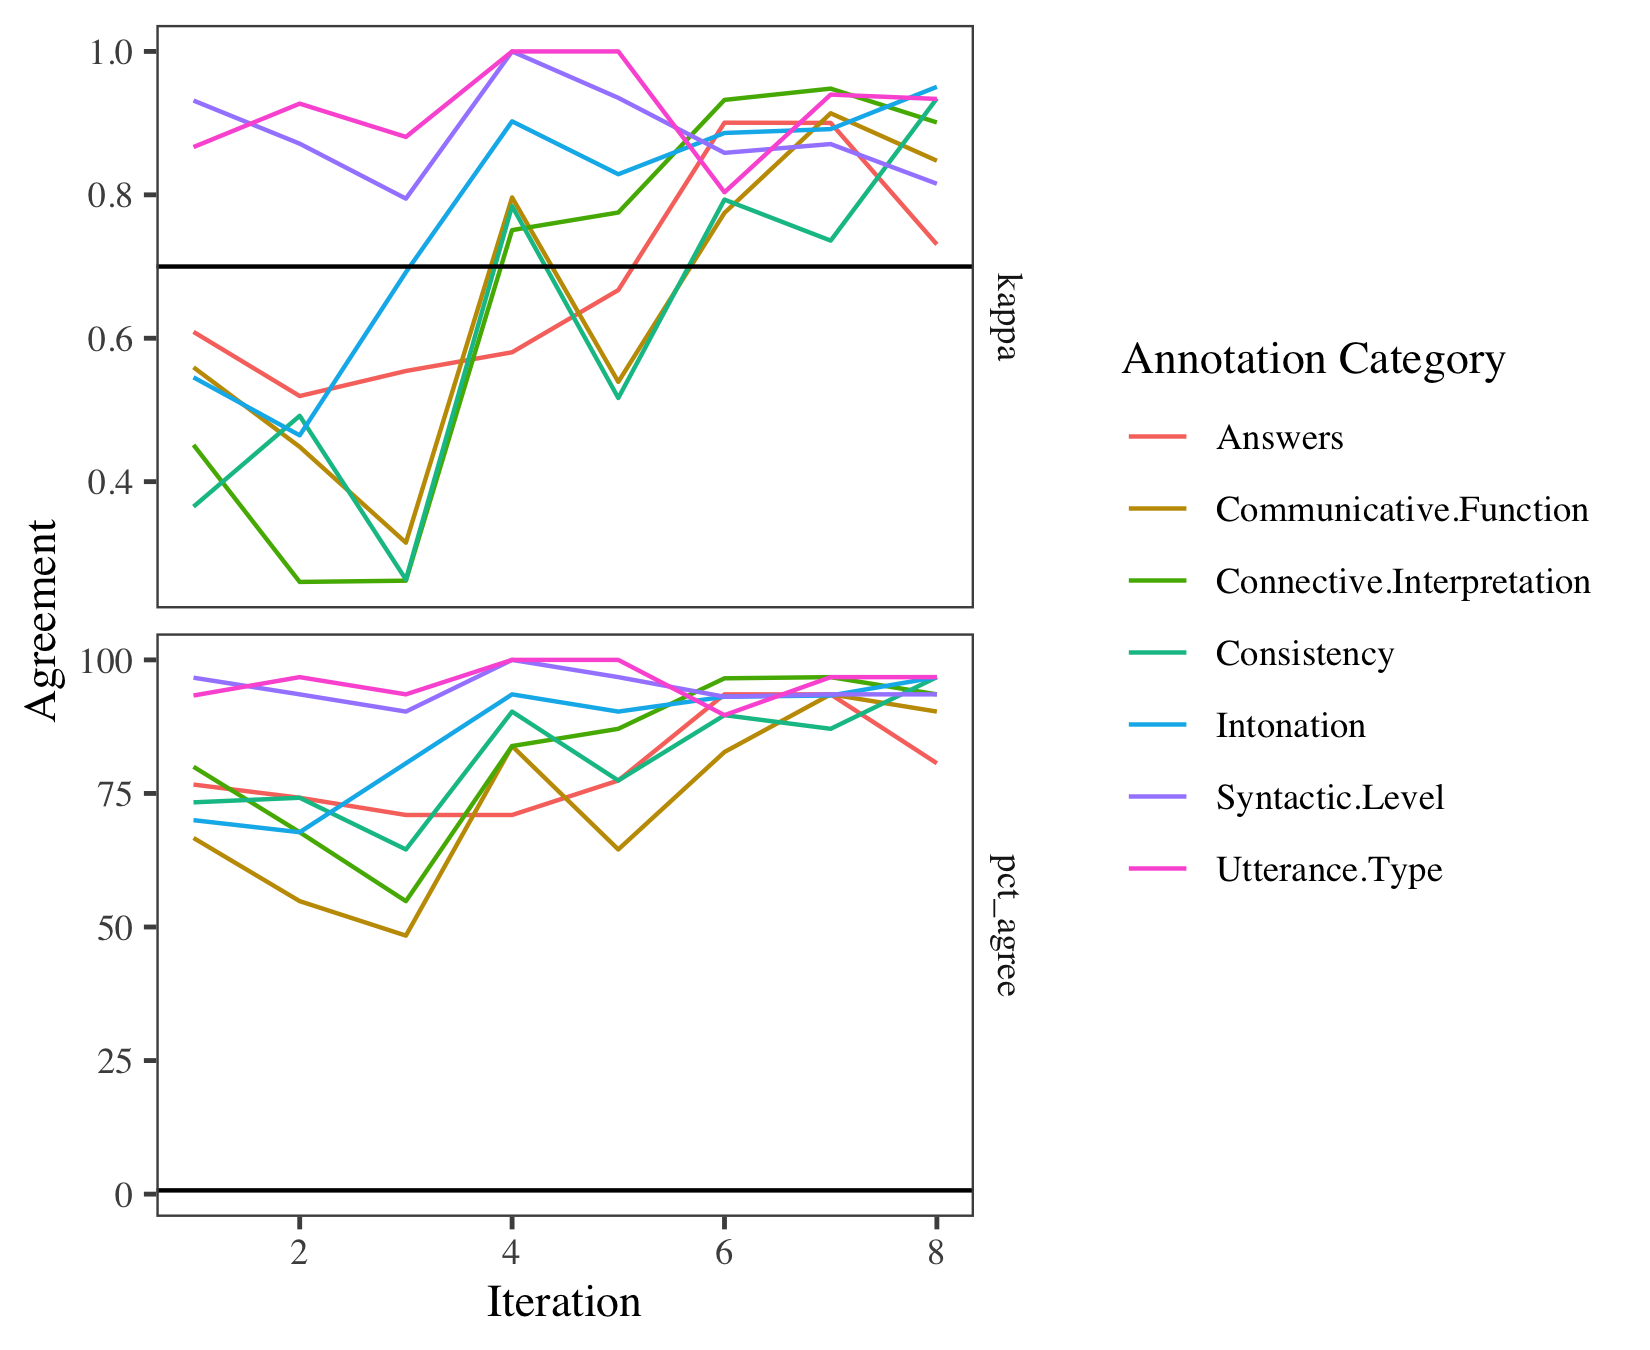
\includegraphics{figs/oReliabilityPlot-1} 

}

\caption{Inter-annotator agreement for disjunction examples.}\label{fig:oReliabilityPlot}
\end{figure}

Agreement in the following three categories showed substantial improvement after better and more precise definitions and annotation criteria were developed: connective interpretation, intonation, and communicative function. First, connective interpretation showed major improvements after annotators developed more precise criteria for selecting the propositions under discussion and separately wrote down the two propositions connected by the connective word. For example, if the original utterance was \enquote{do you want milk or juice?}, the annotators wrote \enquote{you want milk, you want juice} as the two propositions under discussion. This exercise clarified the exact propositions under discussion and sharpened annotator intuitions with respect to the connective interpretation that is communicated by the utterance. Second, annotators improved agreement on intonation by reconstructing an utterance's intonation for all three intonation categories. For example, the annotator would examine the same sentence \enquote{do you want coffee or tea?} with a rise-fall, a rise, and a flat intonation. Then the annotator would listen to the actual utterance and see which one most resembled the actual utterance. This method helped annotators judge the intonation of an utterance more accurately. Finally, agreement on communicative functions improved as the definitions were made more precise. For example, the definition of \enquote{directives} in Table \ref{tab:speechActs} explicitly mentions the difference between \enquote{directives} and \enquote{options}. Clarifying the definitions of communicative functions helped improve annotator agreement.

Inter-annotator reliability for conjunction was calculated in the same way. Two different annotators coded 300 utterances of \emph{and}. Inter-annotator reliability was calculated over 10 iterations of 30 examples. Figure \ref{fig:andReliabilityPlot} shows the percentage agreement between the annotators as well as the kappa values for each iteration. Despite high percentage agreement between annotators, the kappa values did not pass the set threshold of 0.7 in three consecutive iterations. This paradoxical result is mainly due to a property of kappa. An imbalance in the prevalence of annotation categories can drastically lower its value. When one category is extremely common with high agreement while other categories are rare, kappa will be low (Cicchetti \& Feinstein, 1990; Feinstein \& Cicchetti, 1990). In almost all annotated categories for conjunction, there was one class that was extremely prevalent. In such cases, it is more informative to look at the class specific agreement for the prevalent category than the overall agreement measured by Kappa (Cicchetti \& Feinstein, 1990; Feinstein \& Cicchetti, 1990).

\begin{figure}[tb]

{\centering 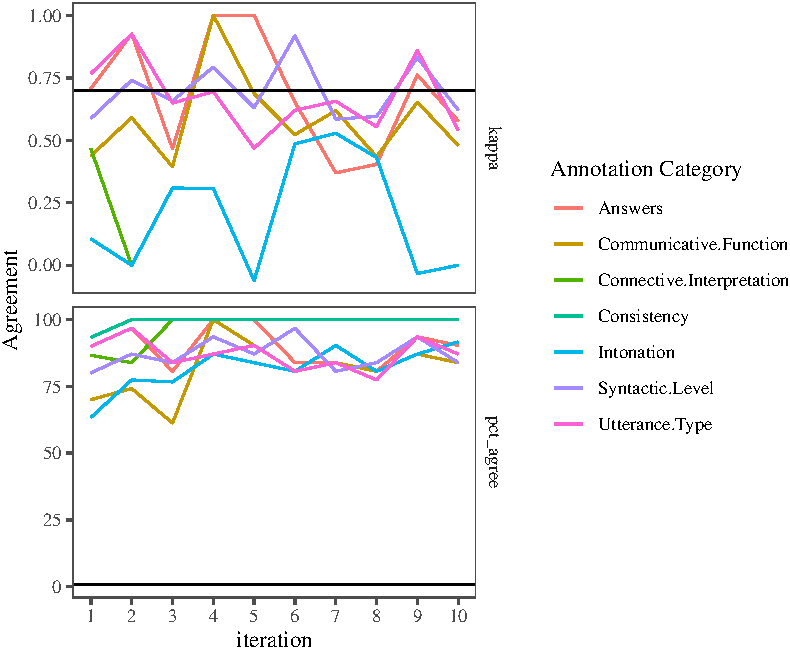
\includegraphics{figs/andReliabilityPlot-1} 

}

\caption{Inter-annotator agreement for conjunction examples.}\label{fig:andReliabilityPlot}
\end{figure}

Table \ref{tab:andAgreeStats} lists the dominant classes as well as their prevalence, the values of class specific agreement index, and category agreement index (Kappa). Class specific agreement index is defined as \(2n_{ii}/n_{i.}+n_{.i}\), where \(i\) represents the class's row/column number in the category's confusion matrix, \(n\) the number of annotations in a cell, and the dot ranges over all the row/column numbers (Fleiss, Levin, \& Paik, 2013, p. 600; Ubersax, 2009). The class specific agreement indices are high for all the most prevalent classes showing that the annotators had very high agreement on these class, even though the general agreement index (Kappa) was often low. The most extreme case is the category \enquote{consistency} where almost all instances were annotated as \enquote{consistent} with perfect class specific agreement but low overall Kappa. In the case of utterance type and syntactic level where the distribution of instances across classes was more even, the general index of agreement Kappa is also high. In general, examples of conjunction showed little variability across annotation categories and mostly fell into one class within each category. Annotators had high agreement for these dominant classes.

\begin{table}

\caption{\label{tab:andAgreeStats}Most prevalent annotation class in each annotation category with the values of class agreement indeces and category agreement indeces (Kappa).}
\centering
\begin{tabular}[t]{l|l|r|r|r}
\hline
Annotation Category & Class & Prevalence & Class Agreement Index & Kappa\\
\hline
intonation & flat & 0.86 & 0.89 & 0.24\\
\hline
interpretation & AND & 0.96 & 0.98 & 0.39\\
\hline
answer & NA & 0.84 & 0.94 & 0.67\\
\hline
utterance\_type & declarative & 0.76 & 0.94 & 0.70\\
\hline
communicative\_function & description & 0.77 & 0.90 & 0.59\\
\hline
syntactic\_level & clausal & 0.67 & 0.91 & 0.70\\
\hline
consistency & consistent & 0.99 & 1.00 & 0.50\\
\hline
\end{tabular}
\end{table}

\setlength{\parindent}{-0.5in}
\setlength{\leftskip}{0.5in}

\hypertarget{refs}{}
\leavevmode\hypertarget{ref-braine1981development}{}%
Braine, M. D., \& Rumain, B. (1981). Development of comprehension of ``or'': Evidence for a sequence of competencies. \emph{Journal of Experimental Child Psychology}, \emph{31}(1), 46--70.

\leavevmode\hypertarget{ref-breiman2001random}{}%
Breiman, L. (2001). Random forests. \emph{Machine Learning}, \emph{45}(1), 5--32.

\leavevmode\hypertarget{ref-breiman2017classification}{}%
Breiman, L. (2017). \emph{Classification and regression trees}. London: Routledge.

\leavevmode\hypertarget{ref-brown1957linguistic}{}%
Brown, R. (1957). Linguistic determinism and the part of speech. \emph{The Journal of Abnormal and Social Psychology}, \emph{55}(1), 1.

\leavevmode\hypertarget{ref-chierchia2001acquisition}{}%
Chierchia, G., Crain, S., Guasti, M. T., Gualmini, A., \& Meroni, L. (2001). The acquisition of disjunction: Evidence for a grammatical view of scalar implicatures. In \emph{Proceedings of the 25th Boston University conference on language development} (pp. 157--168). Somerville, MA: Cascadilla Press.

\leavevmode\hypertarget{ref-chierchia2004semantic}{}%
Chierchia, G., Guasti, M. T., Gualmini, A., Meroni, L., Crain, S., \& Foppolo, F. (2004). Semantic and pragmatic competence in children's and adults' comprehension of or. In I. Noveck \& D. Sperber (Eds.), \emph{Experimental pragmatics} (pp. 283--300). Basingstoke: Palgrave Macmillan.

\leavevmode\hypertarget{ref-cicchetti1990high}{}%
Cicchetti, D. V., \& Feinstein, A. R. (1990). High agreement but low kappa: II. Resolving the paradoxes. \emph{Journal of Clinical Epidemiology}, \emph{43}(6), 551--558.

\leavevmode\hypertarget{ref-crain2012emergence}{}%
Crain, S. (2012). \emph{The emergence of meaning}. Cambridge: Cambridge University Press.

\leavevmode\hypertarget{ref-crain2000acquisition}{}%
Crain, S., Gualmini, A., \& Meroni, L. (2000). The acquisition of logical words. \emph{LOGOS and Language}, \emph{1}, 49--59.

\leavevmode\hypertarget{ref-demuth2006word}{}%
Demuth, K., Culbertson, J., \& Alter, J. (2006). Word-minimality, epenthesis and coda licensing in the early acquisition of English. \emph{Language and Speech}, \emph{49}(2), 137--173.

\leavevmode\hypertarget{ref-feinstein1990high}{}%
Feinstein, A. R., \& Cicchetti, D. V. (1990). High agreement but low kappa: I. The problems of two paradoxes. \emph{Journal of Clinical Epidemiology}, \emph{43}(6), 543--549.

\leavevmode\hypertarget{ref-fisher2010syntactic}{}%
Fisher, C., Gertner, Y., Scott, R. M., \& Yuan, S. (2010). Syntactic bootstrapping. \emph{Wiley Interdisciplinary Reviews: Cognitive Science}, \emph{1}(2), 143--149.

\leavevmode\hypertarget{ref-fleiss2013statistical}{}%
Fleiss, J. L., Levin, B., \& Paik, M. C. (2013). \emph{Statistical methods for rates and proportions}. New York: John Wiley \&amp; Sons.

\leavevmode\hypertarget{ref-geurts2006exclusive}{}%
Geurts, B. (2006). Exclusive disjunction without implicatures. \emph{Ms., University of Nijmegen}.

\leavevmode\hypertarget{ref-gleitman1990structural}{}%
Gleitman, L. (1990). The structural sources of verb meanings. \emph{Language Acquisition}, \emph{1}(1), 3--55.

\leavevmode\hypertarget{ref-goodman2008does}{}%
Goodman, J. C., Dale, P. S., \& Li, P. (2008). Does frequency count? Parental input and the acquisition of vocabulary. \emph{Journal of Child Language}, \emph{35}(3), 515--531.

\leavevmode\hypertarget{ref-grice1989studies}{}%
Grice, H. P. (1989). \emph{Studies in the way of words}. Cambridge, MA: Harvard University Press.

\leavevmode\hypertarget{ref-gualminicrain2002}{}%
Gualmini, A., \& Crain, S. (2002). Why no child or adult must learn de Morgan's laws. In \emph{Proceedings of the Boston University conference on language development}. Somerville, MA: Cascadilla Press.

\leavevmode\hypertarget{ref-gualmini2000}{}%
Gualmini, A., Crain, S., \& Meroni, L. (2000a). Acqisition of disjunction in conditional sentences. In \emph{Proceedings of the boston university conference on language development}.

\leavevmode\hypertarget{ref-gualmini2000inclusion}{}%
Gualmini, A., Meroni, L., \& Crain, S. (2000b). The inclusion of disjunction in child language: Evidence form modal verbs. In \emph{Proceedings of the North East Linguistic Society 30} (Vol. 30). Amherst, MA: GLSA.

\leavevmode\hypertarget{ref-haspelmath2007}{}%
Haspelmath, M. (2007). Coordination. In T. Shopen (Ed.), \emph{Language typology and linguistic description,} Cambridge: Cambridge University Press.

\leavevmode\hypertarget{ref-ho1995random}{}%
Ho, T. K. (1995). Random decision forests. In \emph{Proceedings of the third international conference on document analysis and recognition} (Vol. 1, pp. 278--282). Washington, DC, USA: IEEE Computer Society.

\leavevmode\hypertarget{ref-johansson1975preschool}{}%
Johansson, B. S., \& Sjolin, B. (1975). Preschool children's understanding of the coordinators ``and'' and ``or''. \emph{Journal of Experimental Child Psychology}, \emph{19}(2), 233--240.

\leavevmode\hypertarget{ref-kamp1973free}{}%
Kamp, H. (1973). Free choice permission. In \emph{Proceedings of the Aristotelian society} (Vol. 74, pp. 57--74).

\leavevmode\hypertarget{ref-levy1994words}{}%
Levy, E., \& Nelson, K. (1994). Words in discourse: A dialectical approach to the acquisition of meaning and use. \emph{Journal of Child Language}, \emph{21}(02), 367--389.

\leavevmode\hypertarget{ref-macwhinney2000childes}{}%
MacWhinney, B. (2000). \emph{The CHILDES project: The database} (Vol. 2). Mahwah, NJ: Erlbaum.

\leavevmode\hypertarget{ref-morris2008logically}{}%
Morris, B. J. (2008). Logically speaking: Evidence for item-based acquisition of the connectives ``and'' and ``or''. \emph{Journal of Cognition and Development}, \emph{9}(1), 67--88.

\leavevmode\hypertarget{ref-neisser1962hierarchies}{}%
Neisser, U., \& Weene, P. (1962). Hierarchies in concept attainment. \emph{Journal of Experimental Psychology}, \emph{64}(6), 640.

\leavevmode\hypertarget{ref-notley2012notevery}{}%
Notley, A., Thornton, R., \& Crain, S. (2012a). English-speaking children's interpretation of disjunction in the scope of ``not every''. \emph{Biolinguistics}, \emph{6}(1), 32--69.

\leavevmode\hypertarget{ref-notley2012children}{}%
Notley, A., Zhou, P., Jensen, B., \& Crain, S. (2012b). Children's interpretation of disjunction in the scope of ``before'': A comparison of English and Mandarin. \emph{Journal of Child Language}, \emph{39}(03), 482--522.

\leavevmode\hypertarget{ref-pedregosa2011scikit}{}%
Pedregosa, F., Varoquaux, G., Gramfort, A., Michel, V., Thirion, B., Grisel, O., \ldots{} others. (2011). Scikit-learn: Machine learning in python. \emph{Journal of Machine Learning Research}, \emph{12}(Oct), 2825--2830.

\leavevmode\hypertarget{ref-pruitt2013interpretation}{}%
Pruitt, K., \& Roelofsen, F. (2013). The interpretation of prosody in disjunctive questions. \emph{Linguistic Inquiry}, \emph{44}(4), 632--650.

\leavevmode\hypertarget{ref-sanchez2018childes}{}%
Sanchez, A., Meylan, S., Braginsky, M., MacDonald, K., Yurovsky, D., \& Frank, M. C. (2018). Childes-db: A flexible and reproducible interface to the child language data exchange system. PsyArXiv. Retrieved from \url{psyarxiv.com/93mwx}

\leavevmode\hypertarget{ref-sison1995simultaneous}{}%
Sison, C. P., \& Glaz, J. (1995). Simultaneous confidence intervals and sample size determination for multinomial proportions. \emph{Journal of the American Statistical Association}, \emph{90}(429), 366--369.

\leavevmode\hypertarget{ref-tomasello2003constructing}{}%
Tomasello, M. (2003). \emph{Constructing a language: A usage-based theory of language acquisition}. Harvard University Press.

\leavevmode\hypertarget{ref-ubersax2009}{}%
Ubersax, J. (2009). Retrieved from \url{http://www.john-uebersax.com/stat/raw.htm}

\leavevmode\hypertarget{ref-von1968essay}{}%
Von Wright, G. H. (1968). An essay in deontic logic and the general theory of action.


\end{document}
